\chapter[Remote Observations: Early-stages and Later-stages of Eruption]{Remote Observations\\\LARGE Early-stages and Later-stages of Eruption}
\label{chapter2}
This chapter covers three main topics related to EUV waves and CMEs. Firstly, it focuses on the kinematics of CBFs in both the lower and middle/outer coronas, along with an examination of coronal plasma conditions during these eruptions. Additionally, it discusses my contributions to testing and debugging the \textit{Wavetrack} Python library, developed by \citet{stepanyuk_2022}, for detecting and tracking solar features using wavelet transforms and filtering techniques. Lastly, it examines the research led by \citet{miteva_2023} regarding the connection between reconstructed 3D CME models and geomagnetic storm intensity, emphasizing the importance of accurate 3D modeling for space weather forecasting. The chapter will present the results of each topic individually, followed by a combined discussion and concluding remarks.

\section{Introduction}
CMEs are prominent indicators of solar activity, observable through various wavelengths including white light, UV, and radio \citep{vourlidas_2003, zhang_2006, bein_2011, bastian_2001, veronig_2010}. Early CME phases are effectively observed in Extreme Ultraviolet (EUV) light, facilitated by instruments like AIA aboard SDO \citep{lemen_2011, pesnell_2012}. CMEs can induce shock waves in the solar corona, visible as EUV waves or CBFs \citep{thompson_1998, long_2011}.

CBFs are disturbances propagating over the solar disk and limb, often faster than local characteristic speeds, driven primarily by CMEs or solar flares \citep{thompson_1998, veronig_2010, vrsnak_2008, magdaleni_2010, nindos_2011}. They appear as dome-shaped structures in radio and white-light observations, composed of denser plasma and thus appearing brighter in images \citep{pick_2006, nindos_2008, thompson_2009}.

Studies have clarified CBF characteristics both on the solar disk and off the limb, confirming their wave-like nature \citep{nitta_2013, long_2011, olmedo_2012}. Observations from instruments like LASCO onboard SOHO have extended shock wave investigations beyond 2.5 \rsun \citep{domingo_1995, vourlidas_2003}. While EUV observations link CMEs and EUV waves, understanding shock waves in EUV remains incomplete \citep{patsourakos_2009, kozarev_2011}. Emission measure modeling using AIA's EUV channels provides insights into temperature and density changes in the wavefront's sheath \citep{kozarev_2011}. Multi-wavelength observations from SOHO/LASCO and SDO/AIA instruments have revealed valuable information about CBF properties near the Sun \citep{warmuth_2015}.
Factors such as nearby active regions or coronal holes can distort CBF morphology, and a connection between CBFs and chromospheric disturbances known as Moreton waves has been established \citep{ofman_2002, mann_2003, piantschitsch_2018, thompson_1999b}.

In this study, I analyzed 26 CBF events up to \almost17\rsun using observations and modeling tools from the Solar Particle Radiation Environment Analysis and Forecasting--Acceleration and Scattering Transport (SPREAdFAST) framework \citep{kozarev_2022}. The study aims to characterize CBF kinematics and estimate ambient plasma properties to understand the relationships between shock and plasma parameters.

\section{EUV Observations}
We conducted a study utilizing data from the SOHO/ERNE instrument, focusing on proton events with energies between 17-22 MeV, spanning from 2010 to 2017. Initially, 216 events were identified, but after stringent selection criteria were applied, 133 events were excluded due to various factors such as the absence of EUV wave associations, CMEs, or flares. This left us with a final set of 26 events for analysis.
The selected events (Table~\ref{table_1}), previously discussed in \citep{kozarev_2022}, were further examined using imagery from the AIA instrument's EUV channel 193 $\AA$. These images, captured at a 24-second cadence, provided the primary input for our analysis within the SPREAdFAST framework.

Detailed information about the selected events, including their start/end times, associated flares, and source locations on the solar disk, was obtained from the Heliophysics Events Knowledge (HEK) database. Notably, the mean latitude and longitude of the CBFs were calculated, along with their distribution across the solar hemispheres and quadrants.
CBFs, observed as faint quasi-spherical sheaths, were primarily visible in the 193 $\AA$ channel. To analyze their evolution, sequences of base-difference images were generated for each event, allowing us to track their propagation over time \citep{vourlidas_2003, ontiveros_2009, kozarev_2011, ma_2011}.

% all events had type III radio bursts.
\begin{table} % updated!
	\caption{List of the CBF events with their associated flares and CMEs.}
	\label{table_1}
	\tiny
	\setlength{\tabcolsep}{7pt} % Adjust column separation
	\renewcommand{\arraystretch}{1.5} % Adjust row height
	\begin{tabularx}{\textwidth}{*{12}{>{\centering\arraybackslash}X}}
		\hline 
		\textbf{ID} & \textbf{Event Date} & \textbf{Flare Start (UT)} & \textbf{Flare Max (UT)} & \textbf{Flare Class} & \textbf{EUV Wave Start (UT)} & \textbf{EUV Wave End (UT)} & \textbf{Source X ($"$)} & \textbf{Source Y ($"$)} & \textbf{CME on} & \textbf{$V_{CME}$} & \textbf{AW} \\
		\hline
		0 & 2010/06/12 & 0:30 & 0:57 & 20 & 0:55 & 1:19 & 633 & 390 & 1:32 & 486 & 119\\
		1 & 2010/08/14 & 9:38 & 10:05 & 4.4 & 9:30 & 10:08 & 697 & -26 & 10:12 & 1205 & 360\\
		2 & 2010/12/31 & 4:18 & 4:25 & 1.3 & 4:15 & 5:01 & 799 & 246 & 5:00 & 363 & 45\\
		3 & 2011/01/28 & 0:44 & 1:03 & 13 & 0:45 & 1:59 & 949 & 218 & 1:26 & 606 & 119\\
		4 & 2011/03/07 & 19:43 & 20:12 & 37 & 19:31 & 22:59 & 614 & 553 & 20:00 & 2125 & 360\\
		5 & 2011/05/11 & 2:23 & 2:43 & 0.81 & 2:20 & 2:35 & 785 & 399 & 2:48 & 745 & 225\\
		6 & 2011/08/04 & 3:41 & 3:57 & 93 & 3:43 & 4:20 & 546 & 200 & 4:12 & 1315 & 360\\
		7 & 2011/08/08 & 18:00 & 18:10 & 35 & 17:45 & 18:43 & 812 & 215 & 18:12 & 1343 & 237\\
		8 & 2012/03/07 & 1:05 & 1:14 & 130 & 0:00 & 0:40 & -475 & 397 & 1:30 & 1825 & 360\\
		9 & 2012/03/13 & 17:12 & 17:41 & 79 & 17:03 & 17:44 & 804 & 352 & 17:36 & 1884 & 360\\
		10 & 2012/07/23 & u & u & u & 2:09 & 2:48 & 912 & -243 & 2:36 & 2003 & 360\\
		11 & 2013/04/21 & u & u & u & 6:35 & 7:35 & 937 & 181 & 7:24 & 919 & 360\\
		12 & 2013/05/13 & 15:48 & 16:05 & 280 & 15:44 & 16:20 & -927 & 186 & 16:08 & 1850 & 360\\
		13 & 2013/05/15 & 1:25 & 1:48 & 120 & 1:06 & 1:50 & -852 & 199 & 1:48 & 1366 & 360\\
		14 & 2013/05/22 & 13:08 & 13:32 & 50 & 12:33 & 13:20 & 875 & 238 & 13:26 & 1466 & 360\\
		15 & 2013/06/21 & 2:30 & 3:14 & 29 & 2:31 & 3:21 & -869 & -268 & 3:12 & 1900 & 207\\
		16 & 2013/10/25 & 7:53 & 8:01 & 170 & 7:53 & 8:29 & -914 & -158 & 8:12 & 587 & 360\\
		17 & 2013/12/12 & 3:11 & 3:36 & 0.22 & 3:03 & 3:33 & 750 & -450 & 3:36 & 1002 & 276\\
		18 & 2013/12/28 & 17:53 & 18:02 & 9.3 & 17:10 & 18:00 & 942 & -252 & 17:36 & 1118 & 360\\
		19 & 2014/07/08 & 16:06 & 16:20 & 65 & 16:06 & 16:51 & -767 & 163 & 16:36 & 773 & 360\\
		20 & 2014/12/05 & 5:28 & 5:37 & 2.1 & 5:42 & 6:21 & 872 & -366 & 6:24 & 534 & 172\\
		21 & 2015/05/12 & 2:15 & 3:02 & 2.6 & 2:18 & 2:49 & 960 & -192 & 2:48 & 772 & 250\\
		22 & 2015/09/20 & 17:32 & 18:03 & 21 & 17:28 & 18:11 & 660 & -429 & 18:12 & 1239 & 360\\
		23 & 2015/10/29 & u & u & u & 2:13 & 2:52 & 951 & -167 & 2:36 & 530 & 202\\
		24 & 2015/11/09 & 12:49 & 13:12 & 39 & 12:51 & 13:27 & -626 & -229 & 13:25 & 1041 & 273\\
		25 & 2017/04/01 & 21:35 & 21:48 & 44 & 21:31 & 22:19 & 761 & 308 & 22:12 & 516 & 115\\
		\hline
	\end{tabularx}
\end{table}

The mean latitude and mean longitude of the CBFs were calculated as 56.35 and 378.04 arcsec, respectively. Additionally, the mean latitudes of CBFs in the northern and southern solar hemispheres were found to be 283.00 and -252.73 arcsec, respectively. As for the mean longitudes, they were -775.71 and 803.11 arcsec on the eastern and western sides, respectively.

To analyze the kinematics of CBFs, the Coronal Analysis of SHocks and Waves framework \citep[CASHeW]{kozarev_2017} was employed. This semi-automated technique involved extracting annular regions from AIA images and mapping them onto polar projections (Fig.~\ref{fig_annplot}). By tracking intensity changes along radial and lateral directions, we could measure the kinematics of the CBFs.

Furthermore, plasma parameters and modeling were performed using information retrieved from the HEK database and Nariaki Nitta's catalog of coronal waves \citep{nitta_2013}. The SPREAdFAST framework facilitated calculations of kinematics, inference of shock parameters, and determination of plasma properties for each event.

\begin{figure}[!htp] % updated!
	\centerline{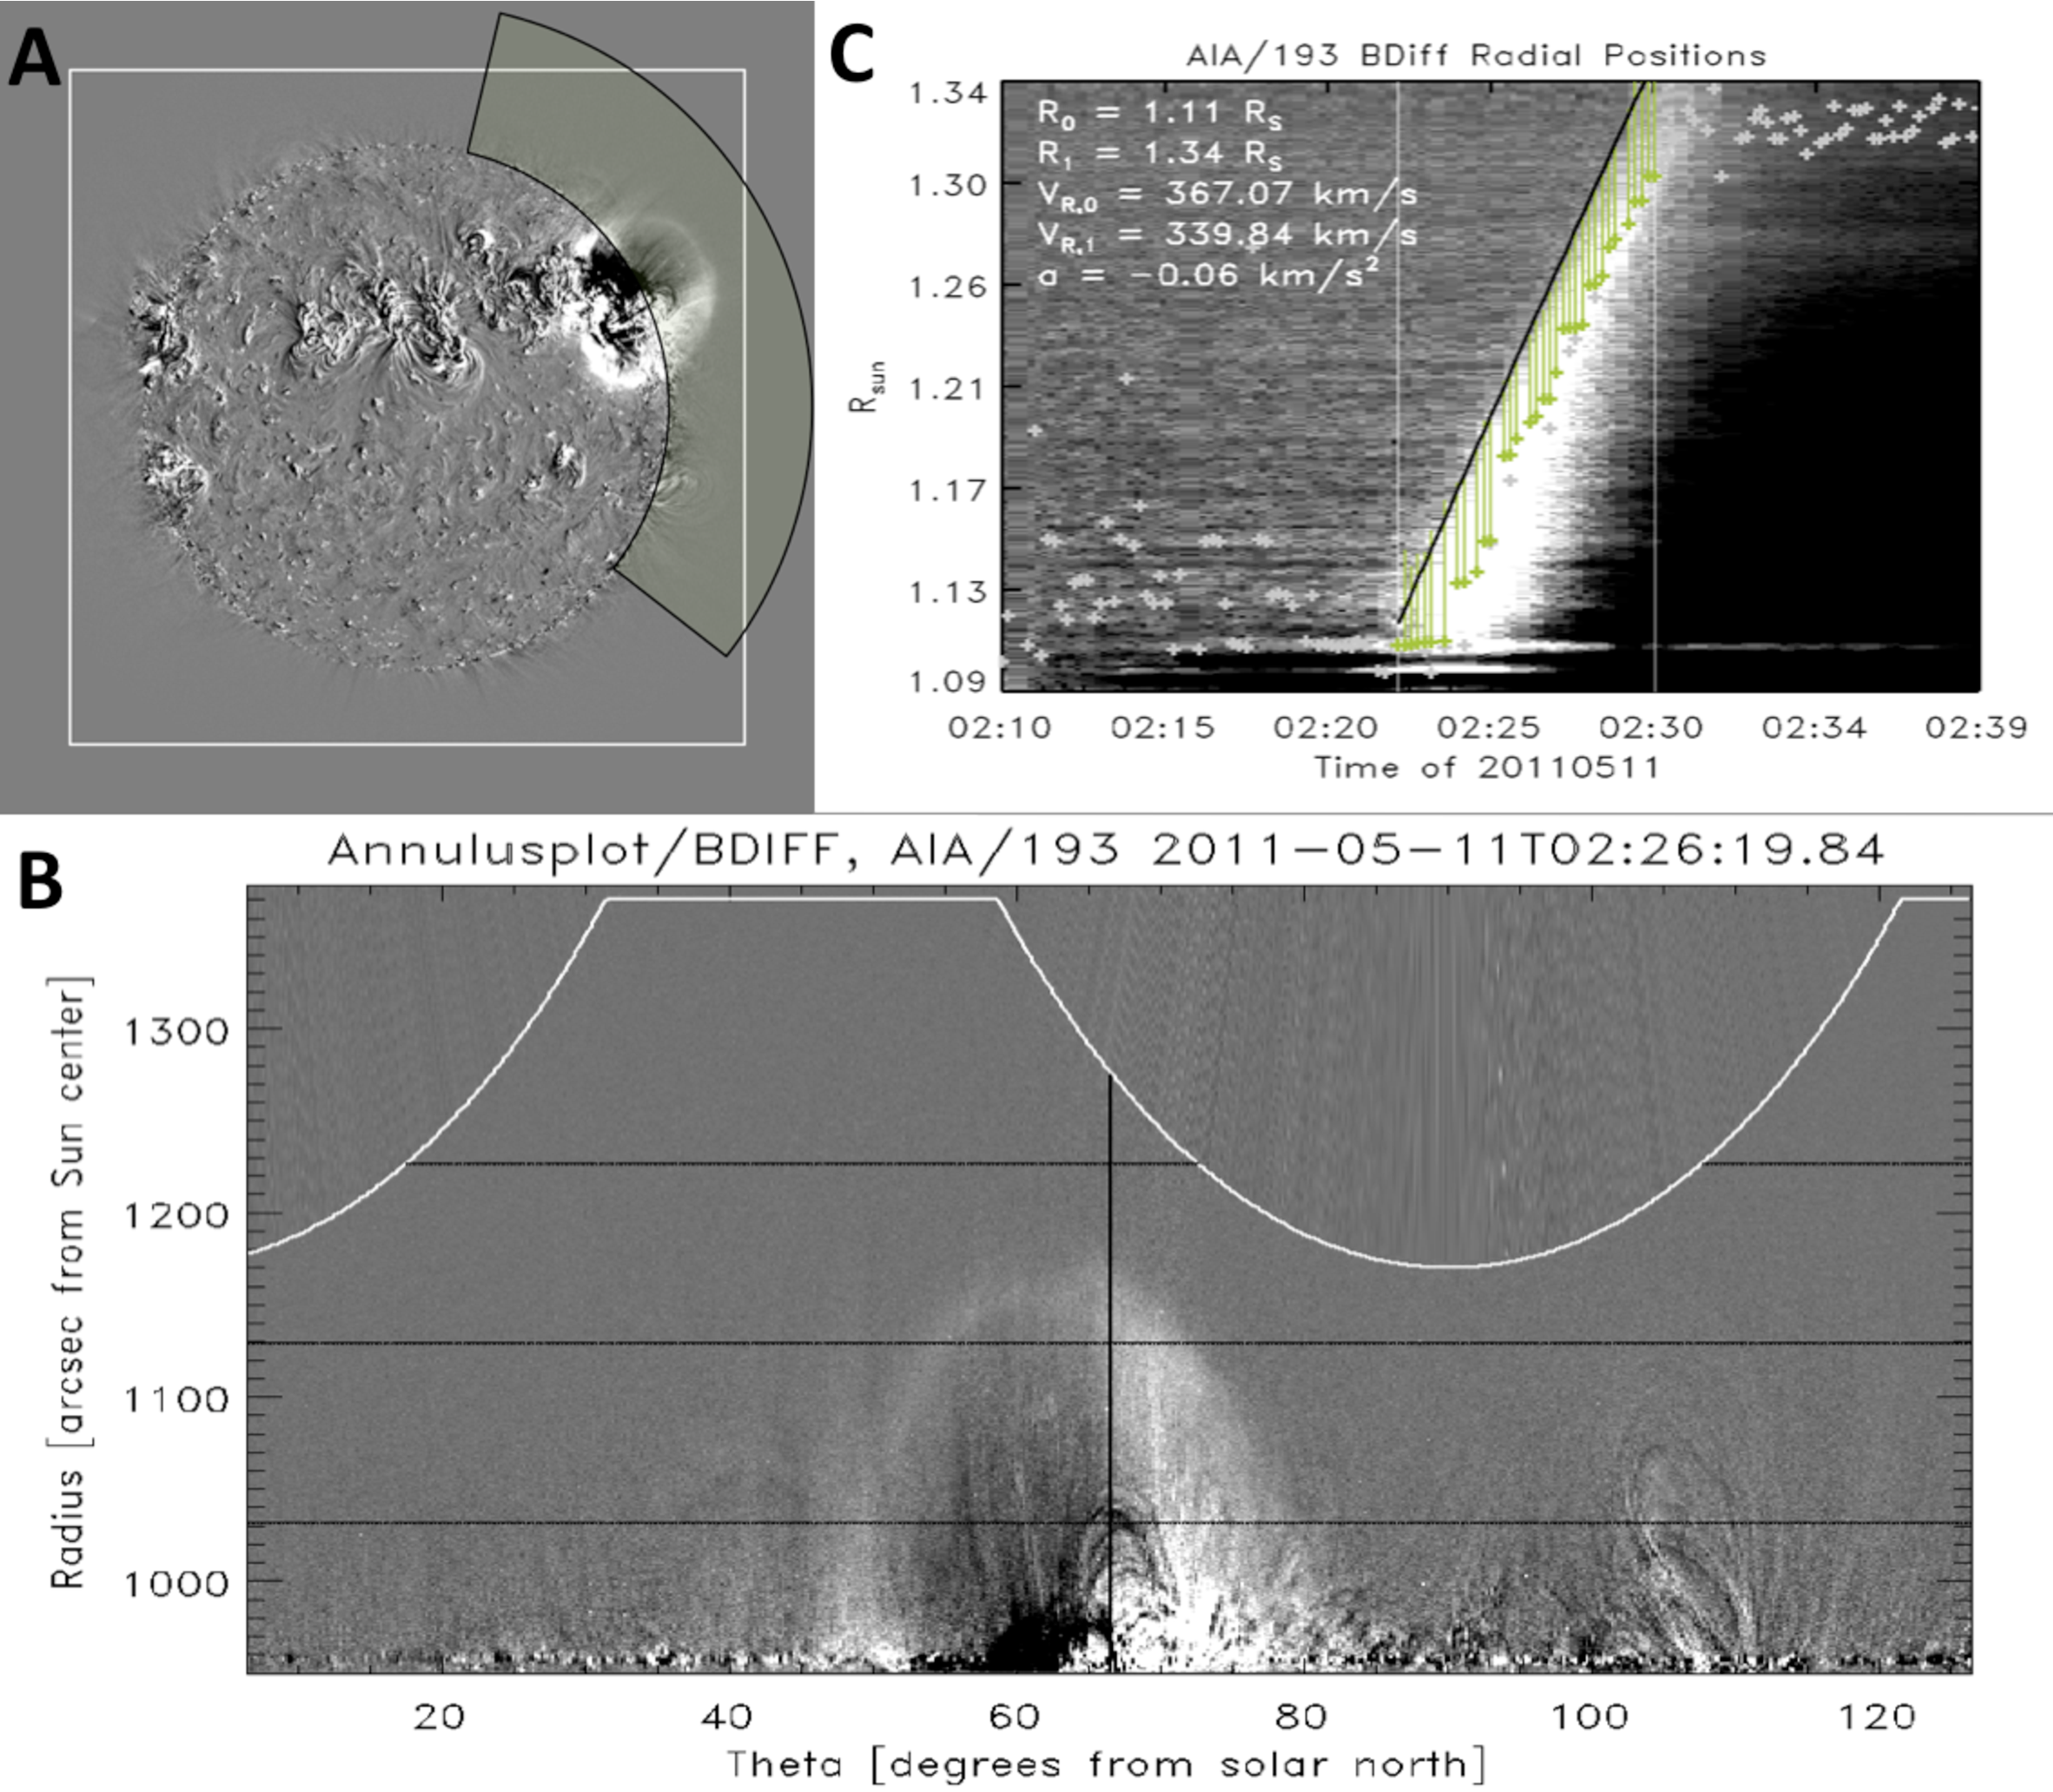
\includegraphics[width=0.9\columnwidth]{chapter2/figs/fig_annplot.pdf}}
	\caption{Illustration for the annulus method used to extract kinematic data from AIA images. (A) shows the full Sun disk with the relevant region highlighted for analysis (green sector). The white box outlines the AIA FOV. (B) displays the extracted annular region mapped onto polar coordinates, with the actual data extent marked by the white curve. Black lines indicate the directions used for measuring radial and lateral motions. (C) shows a stacked plot of intensity along the radial direction, with green markers highlighting intensity peaks and their corresponding distances from the CBF wavefront. The white lines represent the time interval during which the CBF is tracked within the AIA FOV. This figure is curated from \citep{kozarev_2017}.}
	\label{fig_annplot}
\end{figure}

To accurately determine the positions of CBFs over time, we employed several algorithms, including Savitzky-Golay filtering \citep{savitzky_1964} for data smoothening and local minima/maxima ordering for identifying wave positions. Additionally, we manually specified starting and ending times for each CBF event and determined their corresponding heights above the solar limb.

By analyzing intensity values, we defined the positions of CBFs at each time step, considering the front and back of the wave to be at 20\% of the peak intensity. Furthermore, we applied mathematical techniques such as Levenberg-Marquardt least squares minimization \citep{markwardt_2009} and bootstrapping optimization \citep{efron_1979} to fit fourth-order polynomials to the wave positions, enabling measurements of speeds, accelerations, intensities, and thicknesses in both radial and lateral directions.

Finally, measurements of CBF heights and lateral positions were obtained relative to the solar disk and wavefront direction, respectively, providing comprehensive insights into the dynamics of these solar phenomena.
For further reference, the HEK database\footnote{HEK Database: \url{www.lmsal.com/isolsearch}}, Nariaki Nitta's catalog of coronal waves\footnote{Nariaki Nitta's Catalog: \url{https://lmsal.com/nitta/movies/AIA_Waves/index.html}}, and the LASCO CME Catalog\footnote{LASCO CME Catalog: \url{https://cdaw.gsfc.nasa.gov/CME_list/}} were utilized, along with detailed summary plots available in the online SPREAdFAST catalog\footnote{SPREAdFAST Catalog: \url{https://spreadfast.astro.bas.bg/catalog/}}.

\section{Data Analysis and Methods}
The Solar Particle Radiation Environment Analysis and Forecasting–-Acceleration and Scattering Transport (SPREAdFAST) system, developed by \citet{kozarev_2022} and referred to as SPREAdFAST throughout this discussion, operates as a physics-based prototype for forecasting SEP events within the heliosphere. Built upon the CASHeW framework, SPREAdFAST integrates data-driven models to forecast various aspects of SEP events, including arrival times, maximum intensities, and fluxes at different locations in the inner heliosphere. These predictions play a vital role in space weather forecasting, contributing to the protection of assets owned by the European Space Agency (ESA) and aiding satellite operators in making informed decisions to mitigate the impacts of space weather on electronics and human activities in space \citep{kozarev_2022}.

The SPREAdFAST catalog offers summary plots of J-maps and kinematic data for each SEP event, as highlighted by \citet{kozarev_2022}. Additionally, to ensure consistency in lateral kinematic measurements, an averaging technique is applied to data from both lateral left and right flanks, as described by the same authors. Further analysis involves the application of a Savitzky-Golay fit, as outlined in previous work by \citet{kozarev_2019}, and the utilization of analytical models for CME kinematics by \citet{gallagher_2003} and \citet{byrne_2013} to extrapolate smoothed radial positions up to $\sim$17\rsun.

Moving forward, the development of synthetic shock models (S2M) forms the next phase of the study, as mentioned by \citet{kozarev_2022}. These models, operating at a 24-second cadence, are constructed based on extrapolated radial and lateral kinematic results and incorporate major and minor axes of spheroids representing compressive waves. The shock surface is delineated from the onset of the CBF until its nose reaches 10 \rsun and then extended up to 30 \rsun utilizing results from the Magnetohydrodynamic Algorithm outside a Sphere (MAS) synoptic coronal model.

The methodology for estimating shock density jump is detailed by \citet{kozarev_2017}, involving the calculation of differential emission measure (DEM) during and before the event at each shock crossing and timestep. This approach, informed by \citet{cheung_2015}, provides insights into the variation in density across shock structures. Notably, while the density jump within the AIA FOV typically remains below 1.2, regions beyond observational limits are assigned a value of 1.2, assuming the presence of weak shocks.

To facilitate analysis, the synthetic shock model is segmented into distinct regions--the cap representing the shock nose, Zone 1, and Zone 2 representing the shock flanks--as explained by \citet{kozarev_2022}. This segmentation aids in the examination of plasma parameter distributions across different sectors of the shock surface, as depicted in Figure~\ref{fig_segments}.

\begin{figure}[!htp] % updated!
	\centerline{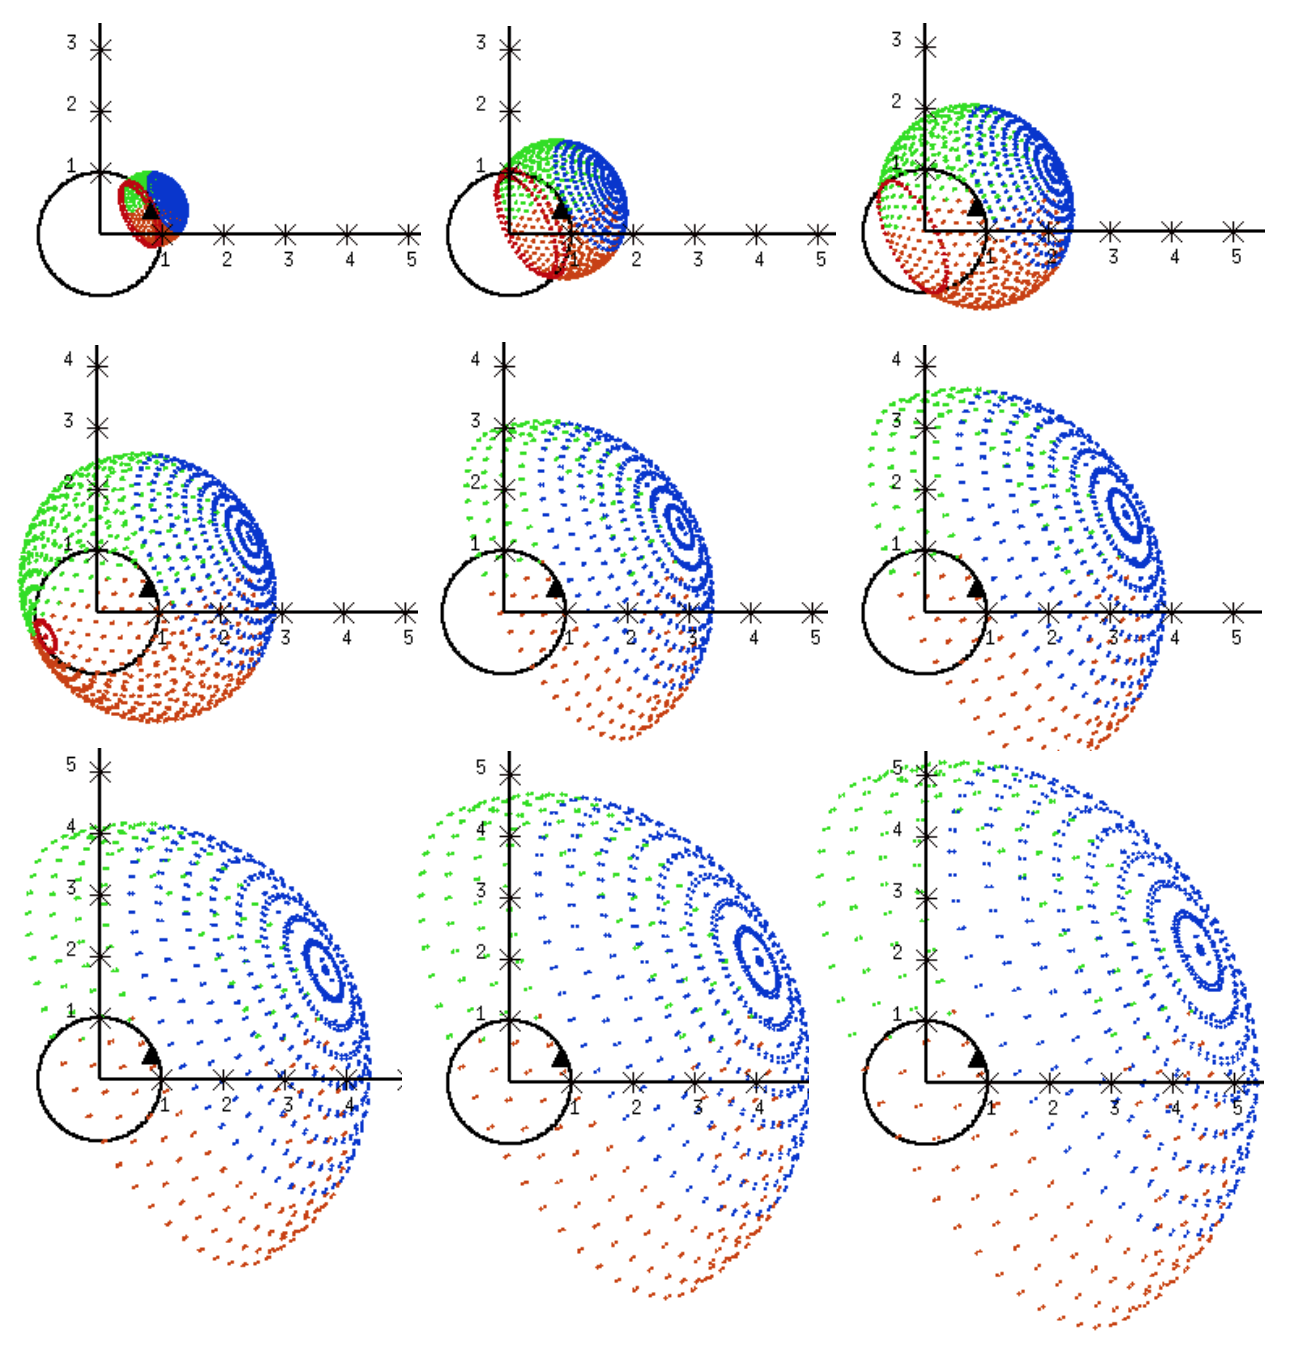
\includegraphics[width=0.5\columnwidth]{chapter2/figs/fig_s2m_segments_geometry.png}}
	\caption{Synthetic shock model divided into three segments; the cap zone in blue and the flank zones are in red and green.}
	\label{fig_segments}
\end{figure}

\section{CBF Kinematics and Geometric Modeling: Case Study May 11, 2011}
In this section, I analyze a case study event in the low corona region and investigate plasma parameters along shock-crossing magnetic field lines in the AIA FOV.

\subsection{Event Context}
The eruption occurred on May 11, 2011, at around 02:20 UT (Fig.~\ref{fig_aia_event}), originating from an active region in the northwestern sector (N18W52). It involved a massive shock wave propelled by a fast partial-halo CME, with a linear speed of 745 \kms, a 2$^{nd}$-order speed at 20\rsun of 776 \kms, and an acceleration of 3.3 m s$^{-2}$. The eruption was accompanied by a weak B8.1 solar flare and an eruptive filament observed by the SDO/AIA instrument.

\begin{figure}[!htp] % updated!
	\centerline{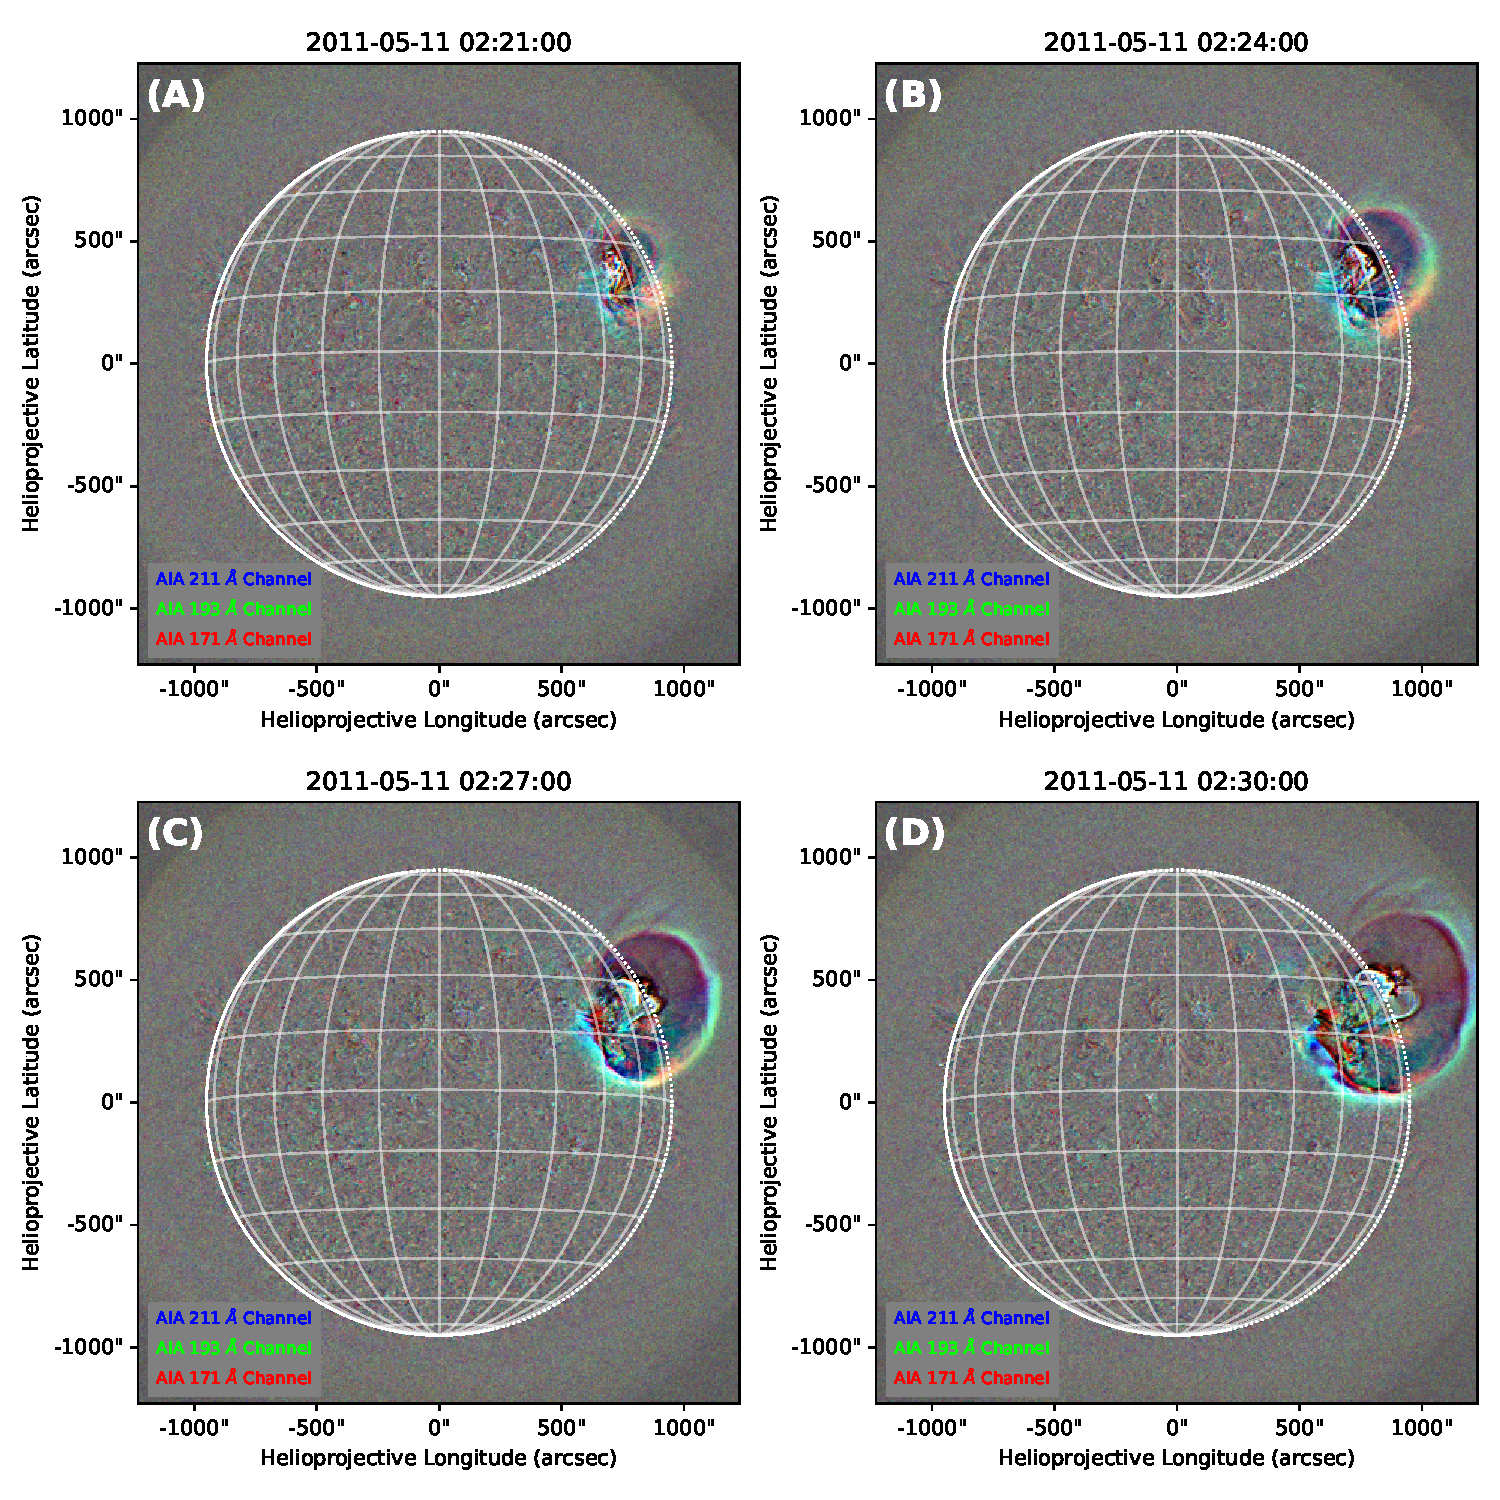
\includegraphics[width=0.8\columnwidth]{chapter2/figs/RGB_panel.pdf}}
	\caption{AIA running-difference images capture a coronal wave evolving over 9 minutes near the Sun's western limb, exhibiting markedly changing intensity and structure as observed in 171, 193, and 211 $\AA$.}
	\label{fig_aia_event}
\end{figure}

Additionally, a type II radio burst was associated with the eruption, observed by the Learmonth spectrogram. Proton fluxes near 1 AU showed an increase, and an SEP event was detected at Earth with onset time of 03:39 UT and a $J_p$ of 0.0133 protons/(cm$^2$ s sr MeV) in the energy channel 17-22 MeV \citep{miteva_2016, miteva_2017}.  $J_p$ is the peak proton intensity after subtracting the pre-event level.

\subsection{Low Corona Part}
To investigate the kinematics of the CBF event, I employed the CASHeW module within the SPREAdFAST framework. The shock wave's asymmetrical evolution is detailed, along with its morphological changes over time. The average speeds and accelerations for the radial and lateral directions are provided (Fig.~\ref{fig_kinematics_110511}), along with a comparison of wave thickness between flanks. The shock surface is divided into segments for further analysis (Fig.~\ref{fig_segments}). Table~\ref{T_110511} provides a summary of the statistical results, and the results for the three segments are summarized in Table~\ref{T_sh_param_110511}.

\begin{figure}[!htp] % updated!
	\centerline{
		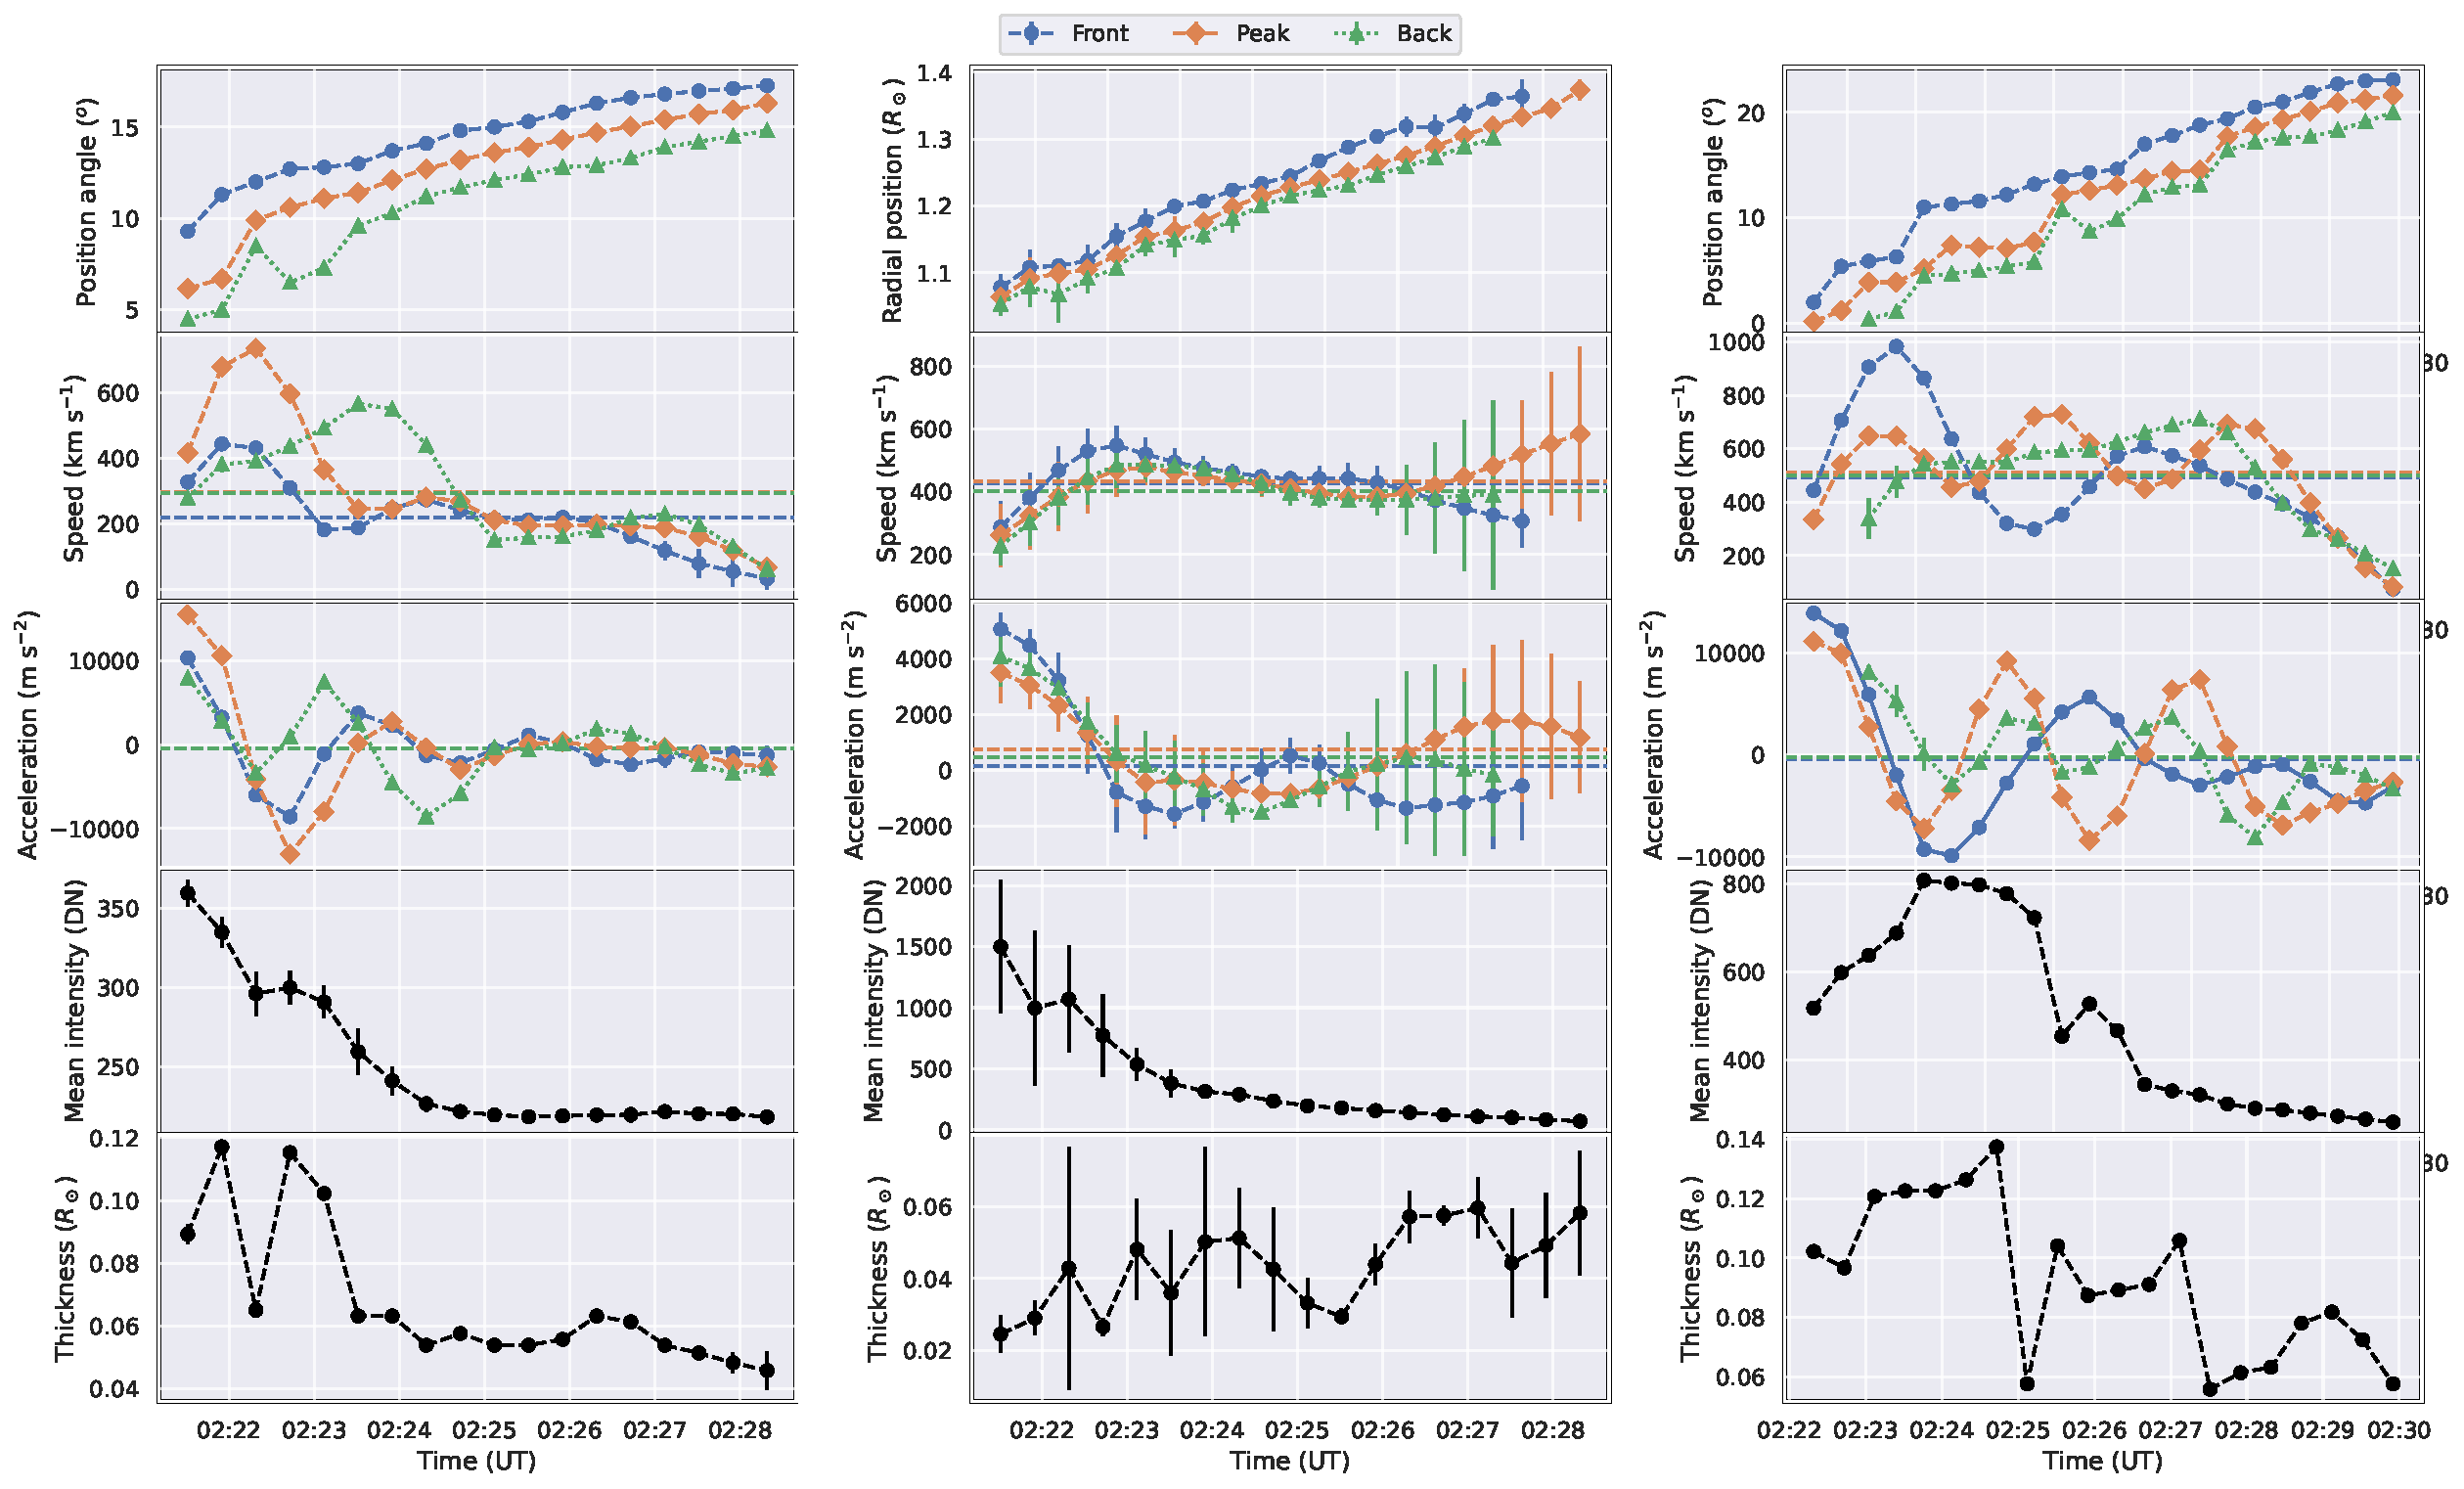
\includegraphics[width=1\textwidth,clip=]{chapter2/figs/euvwave_kinematics_110511_01.pdf}
	}
	\caption{Time-series kinematics of the CBF parameters for the front, peak, and back positions in the AIA FOV, with measurement uncertainties shown as small bars over the data points. The horizontal lines in the speed and acceleration panels denote the mean speeds and accelerations for the wave front, peak, and back with respective colors. The left and right columns represent the lateral kinematic measurements in the left and right flanks of the wave, respectively. The middle column represent the kinematic measurements in the radial direction.}
	\label{fig_kinematics_110511}
\end{figure}

\begin{table}[!htp] % updated!
	\centering
	\caption{Mean values and their standard deviation of the wave parameters in the radial direction and the lateral direction for the left and right flanks, at the front, peak, and back sides of the wave for the event occurred on May 11, 2011, in the SDO/AIA FOV.}
	\label{T_110511}
	\resizebox{\textwidth}{!}{%
		\begin{tabular}{lc|c|c|c}
			\hline
			Parameter                              & Direction  & Front              & Peak                   & Back                 \\ \hline
			\multirow{3}{*}{$<speed>$ \kms}        & Lat. Left  & 218.46 $\pm$ 9.04  & 297.46 $\pm$ 5.45      & 293.94 $\pm$ 9.04    \\ \cline{2-5}
			& Radial     & 427.46 $\pm$ 51.85 & 433.11 $\pm$ 82.86     & 400.81 $\pm$ 83.78   \\ \cline{2-5} 
			& Lat. Right & 494.69 $\pm$ 0.00  & 509.25 $\pm$ 1.02      & 498.97 $\pm$ 9.21    \\ \hline
			\multirow{3}{*}{$<accel.>$ m s$^{-2}$} & Lat. Left  & -414.62 $\pm$ 227.23 & -401.46 $\pm$ 164.62 & -385.77 $\pm$ 227.23 \\ \cline{2-5}
			& Radial     & 147.41 $\pm$ 1009.19 & 758.97 $\pm$ 1287.65 & 485.38 $\pm$ 1365.80 \\ \cline{2-5} 
			& Lat. Right & -415.04 $\pm$ 0.00   & -209.81 $\pm$ 22.32  & -266.68 $\pm$ 250.80 \\ \hline
			\multirow{3}{*}{$<intensity>$ DN}      & Lat. Left  & \multicolumn{3}{c}{250.60 $\pm$ 5.90}               \\ \cline{2-5}
			& Radial     & \multicolumn{3}{c}{403.34 $\pm$ 143.30}             \\ \cline{2-5}
			& Lat. Right & \multicolumn{3}{c}{489.04 $\pm$ 2.86}               \\ \hline
			\multirow{3}{*}{$<thickness>$\rsun}   & Lat. Left  & \multicolumn{3}{c}{0.07 $\pm$ 0.00}                 \\ \cline{2-5}
			& Radial     & \multicolumn{3}{c}{0.04 $\pm$ 0.01}                 \\ \cline{2-5}
			& Lat. Right & \multicolumn{3}{c}{0.09 $\pm$ 0.00}                 \\ \hline
		\end{tabular}%
	}
\end{table}

\begin{table}[!htp] % updated!
	\centering
	\caption{Mean, median, and standard deviation of the shock parameters output, from the interaction of the S2M spheroid with the MAS MHD model results, for the shock's cap and flanks and for the whole shock surface, for the event on May 11, 2011.}
	\label{T_sh_param_110511}
	\begin{tabular}{lcccc}
		\hline
		\multirow{2}{*}{Segment} & \multirow{2}{*}{Parameter} & \multicolumn{3}{c}{Statistics} \\
		&                         & Mean & Median & Stdv \\ \hline
		All & $V_{SHOCK}$ \kms    & 577.77 & 578.39 & 72.79 \\ 
		& $\theta_{BN}$ \degree   & 70.06 & 0.63 & 44.83 \\ 
		& $B_{MAG}$ G             & 0.046 & 0.038 & 0.070 \\ 
		& Density Jump            & 1.193 & 1.188 & 0.185 \\ \hline
		
		Cap & $V_{SHOCK}$ \kms    & 555.18 & 550.86 & 42.46 \\ 
		& $\theta_{BN}$ \degree   & 19.37 & 3.61 & 25.51 \\ 
		& $B_{MAG}$ G             & 0.046 & 0.036 & 0.070 \\ 
		& Density Jump            & 1.193 & 1.188 & 0.015 \\ \hline
		
		Zone 1 & $V_{SHOCK}$ \kms & 613.69 & 609.32 & 59.42 \\ 
		& $\theta_{BN}$ \degree   & 6.46 & 0.21 & 50.92 \\ 
		& $B_{MAG}$ G             & 0.045 & 0.045 & 0.066 \\ 
		& Density Jump            & 1.190 & 1.187 & 0.008 \\ \hline
		
		Zone 2 & $V_{SHOCK}$ \kms & 631.37 & 614.23 & 73.07 \\ 
		& $\theta_{BN}$ \degree   & 0.10 & 0.51 & 10.61 \\ 
		& $B_{MAG}$ G             & 0.046 & 0.029 & 0.071 \\ 
		& Density Jump            & 1.194 & 1.188 & 0.016 \\ \hline
	\end{tabular}
\end{table}

Moreover, shock-crossing magnetic field lines during this event were investigated in \citep{kozarev_2022}, with key plasma parameters analyzed up to 10\rsun. The aspect ratio of the coronal wave's geometry is discussed, along with changes in shock-field angle and magnetic field amplitude over time and radial distance.

\subsection{Middle/Outer Corona Part}
Complementary measurements from the SOHO/LASCO instrument\footnote{LASCO CME Catalog: \url{https://cdaw.gsfc.nasa.gov/CME_list/}} expand the analysis of EUV waves' kinematics in the middle/outer corona. The height-time profile of the CME leading edge associated with the coronal wave is examined, employing fitting models of \citet{gallagher_2003} and \citet{byrne_2013} to analyze the data (Fig.~\ref{fig_height_profile_aialasco_110511}). Insights into the wave's acceleration and speed variation over time and distance from the Sun are provided (Fig.~\ref{fig_rad_kinematics_aialasco_110511}).

\begin{figure}[!htp] % updated!
	\centerline{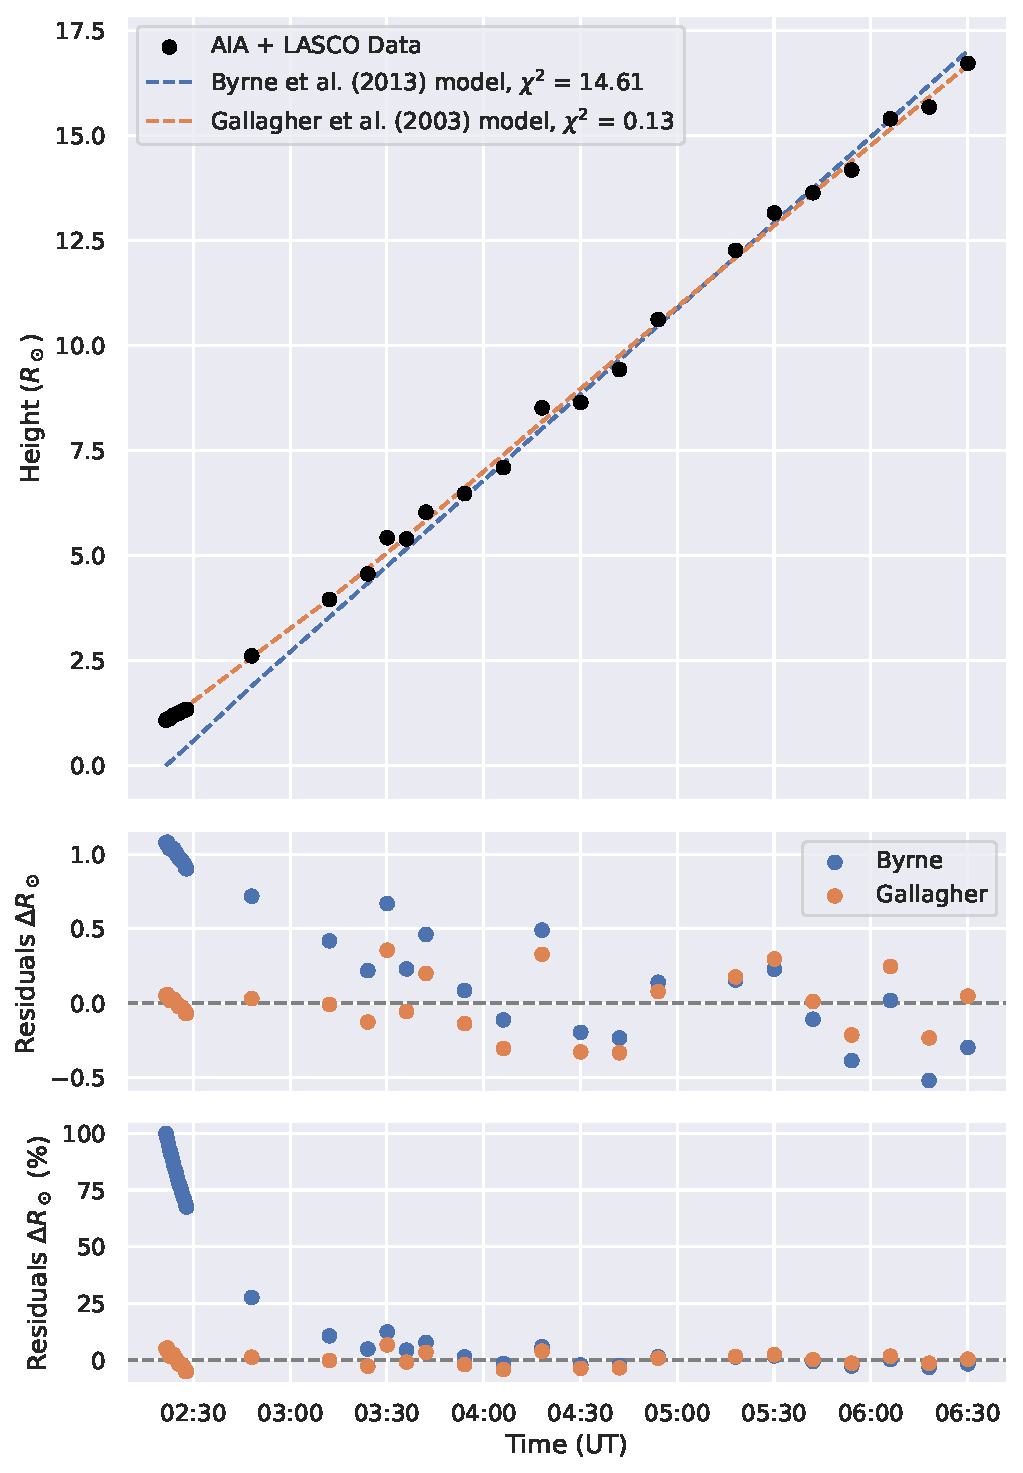
\includegraphics[width=0.7\columnwidth]{chapter2/figs/height_profile_residuals_aia_lasco_110511_01.pdf}}
	\caption{Top panel -- Height-time profile compiled from AIA and LASCO measurements for the event occurred on May 11, 2011, fitted with two CME kinematics models from the photosphere up to 17\rsun. Middle panel -- Difference between the fitting and the real observations. Bottom panel -- Relative residuals in \%.}
	\label{fig_height_profile_aialasco_110511}
\end{figure}

\begin{figure}[!htp] % updated!
	\centerline{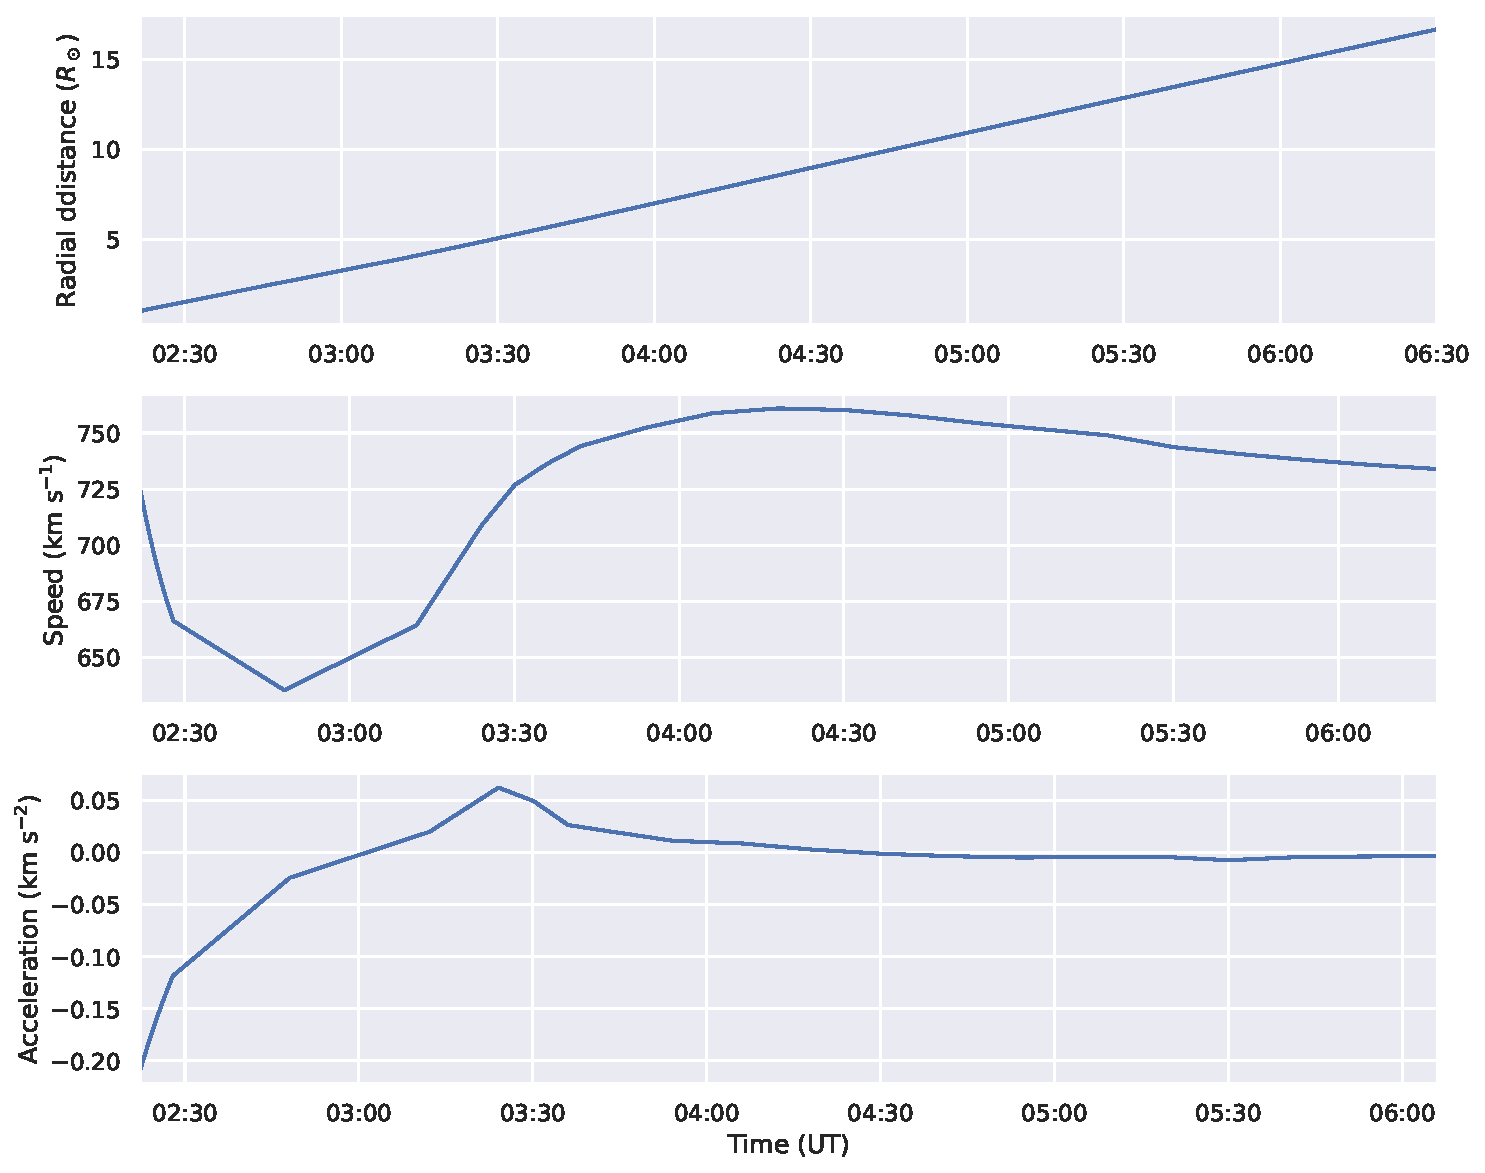
\includegraphics[width=0.8\columnwidth]{chapter2/figs/radial_kinematics_aia_lasco_110511_01.pdf}}
	\caption{Extrapolated radial kinematics for the event occurred on May 11, 2011, based on the ballistic model of \cite{gallagher_2003} up to 17\rsun.}
	\label{fig_rad_kinematics_aialasco_110511}
\end{figure}



\section{Statistical Study}
I conduct a thorough statistical analysis of coronal wave events observed in the AIA and LASCO FOVs, focusing on kinematic characteristics and plasma parameters.

Table~\ref{T_sh_param_all} summarizes statistical parameters related to shock characteristics, such as wave speed, intensity, and thickness in the AIA FOV.
Analysis reveals higher speeds, accelerations, lower mean intensities, and thickness in the radial direction compared to the lateral direction, suggesting early elongation of waves near the Sun.

Figure~\ref{fig_kinematics_spect_hist} illustrates EUV waves' kinematics evolution in the AIA FOV, showing parameter distributions as a function of distance for shock speed, acceleration, wave intensity, and thickness in radial and lateral directions.
Speed and intensity decline with distance due to momentum loss and decreasing plasma densities. All dynamic spectra for individual events are accessible on the SPREAdFAST catalog webpage\footnote{SPREAdFAST Catalog: \url{https://spreadfast.astro.bas.bg/catalog/}}.

\begin{table}[!htp] % updated!
	\centering
	\caption{Statistics of the EUV wave kinematics in the SDO/AIA FOV for the 26 events. LL and LR refer to the lateral left and right flanks, respectively. Rad refer to the radial front direction.}
	\label{T_sh_param_all}
	\resizebox{\textwidth}{!}{%
		\begin{tabular}{lccccccccccccc}
			\hline
			&              & \multicolumn{3}{c}{Speed (\kms)}  & \multicolumn{3}{c}{Accel. (km s$^{-2}$)} & \multicolumn{3}{c}{Intensity (DN)} & \multicolumn{3}{c}{Thickness (\rsun)} \\ \hline
			& Aspect ratio & LL      & Rad     & LR     & LL      & Rad     & LR     & LL       & Rad      & LR      & LL       & Rad      & LR      \\ \hline
			Max    & 2.00         & 1574.81 & 2053.73 & 983.58 & 28.19   & 81.01   & 13.89  & 1348.87  & 2431.95  & 1498.45 & 9.600    & 0.185    & 6.100   \\ \hline
			Min    & 0.84         & 2.11    & 40.30   & 2.30   & -35.24  & -81.01  & -9.89  & 0.53     & 0.17     & 150.30  & 0.027    & 0.018    & 0.022   \\ \hline
			Mean   & 1.87         & 316.17  & 413.60  & 264.50 & -0.15   & 0.98    & 0.13   & 438.99   & 681.46   & 442.46  & 0.715    & 0.059    & 0.231   \\ \hline
			Median & 2.00         & 284.77  & 349.32  & 216.32 & 0.03    & 0.37    & 0.11   & 337.96   & 425.23   & 389.06  & 0.102    & 0.055    & 0.076   \\ \hline
			Stdv.  & 0.33         & 261.01  & 336.11  & 191.13 & 5.53    & 11.08   & 2.05   & 292.26   & 592.78   & 227.10  & 1.721    & 0.030    & 0.776   \\ \hline
		\end{tabular}%
	}
\end{table}

\begin{figure}[!htp] % updated!
	\centerline{
		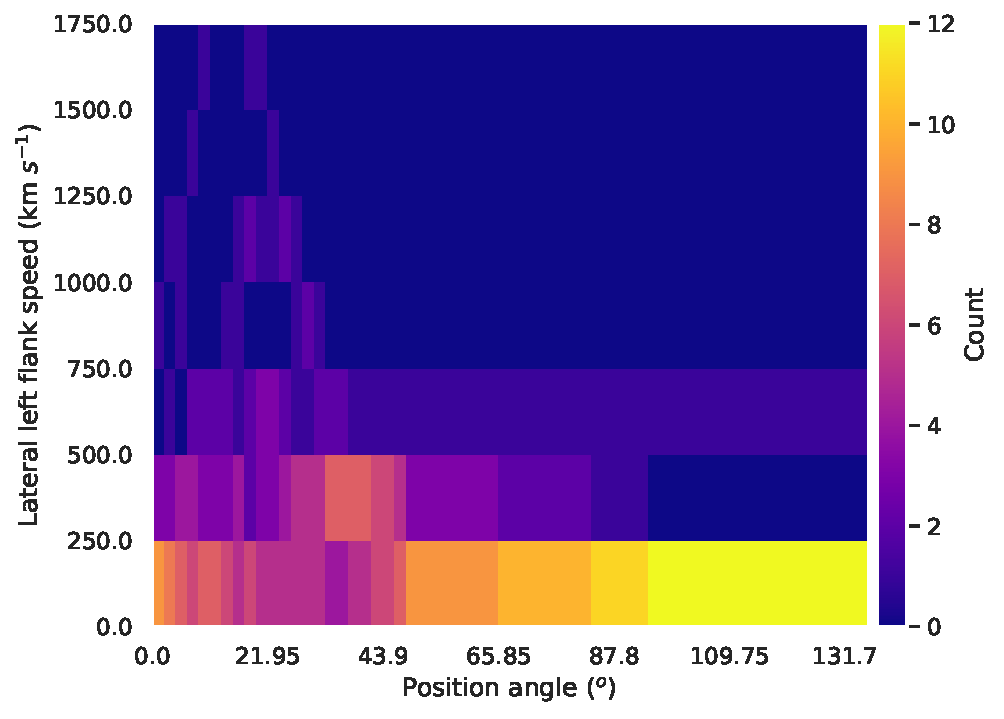
\includegraphics[width=0.32\textwidth,clip=]{chapter2/figs/latleftspd_vs_latleftpos.pdf}
		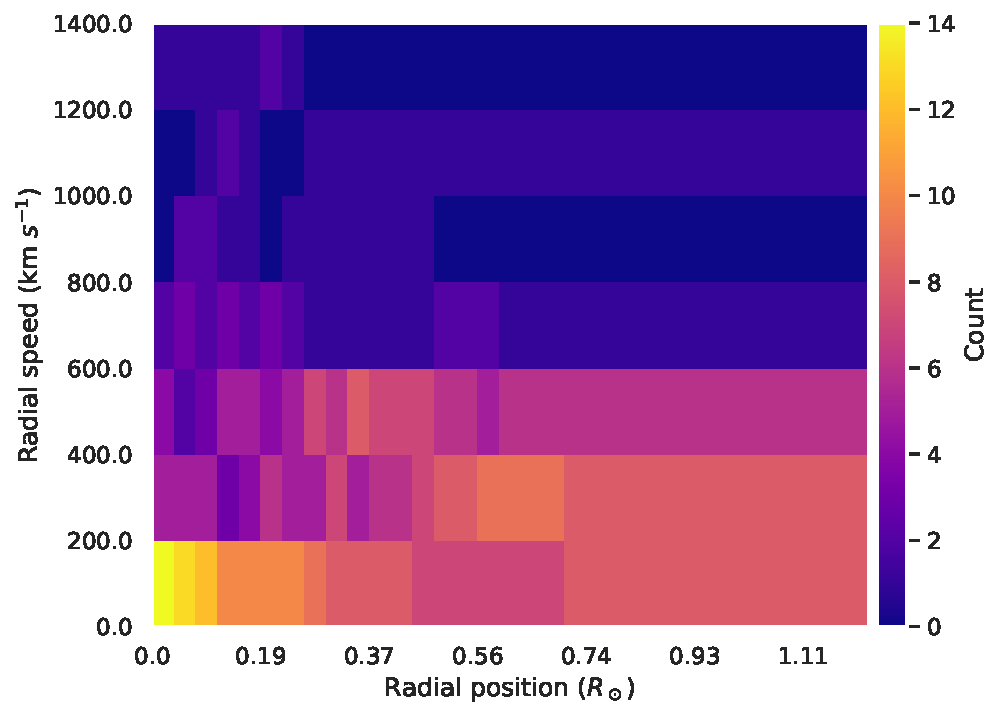
\includegraphics[width=0.32\textwidth,clip=]{chapter2/figs/radspd_vs_radpos.pdf}
		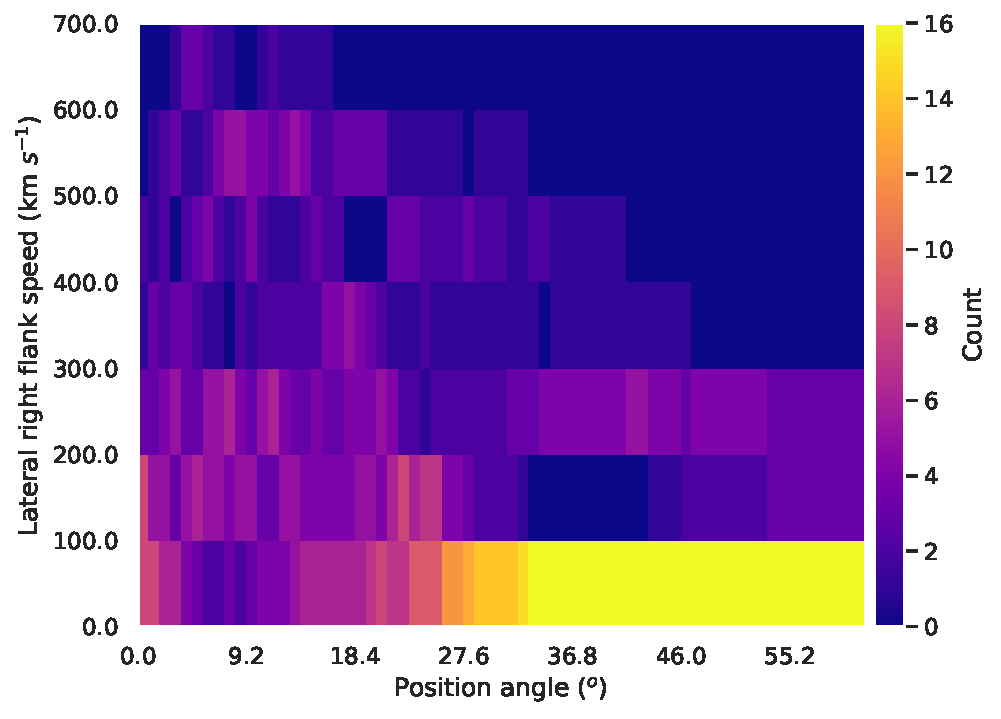
\includegraphics[width=0.32\textwidth,clip=]{chapter2/figs/latrightspd_vs_latrightpos.pdf}
	}
	\centerline{
		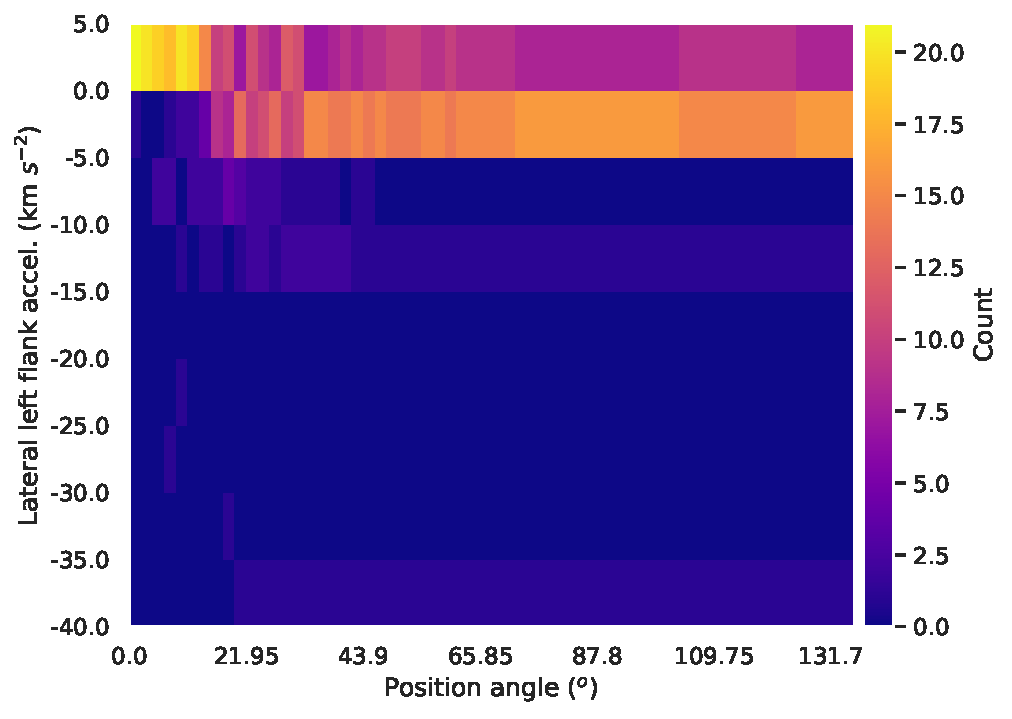
\includegraphics[width=0.32\textwidth,clip=]{chapter2/figs/latleftaccel_vs_latleftpos.pdf}
		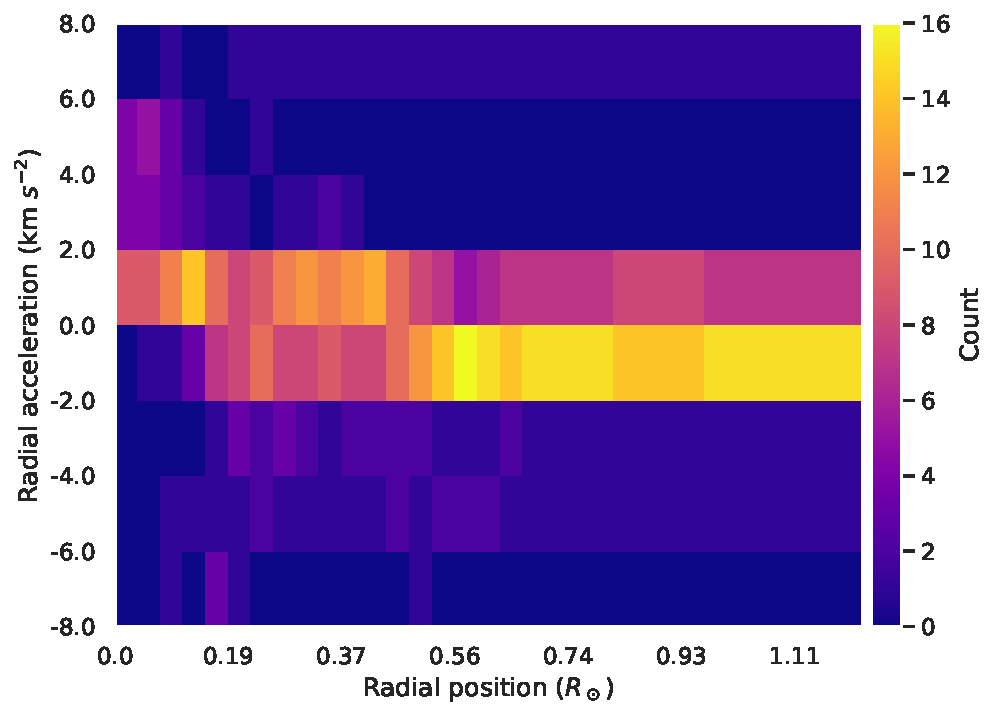
\includegraphics[width=0.32\textwidth,clip=]{chapter2/figs/radaccel_vs_radpos.pdf}
		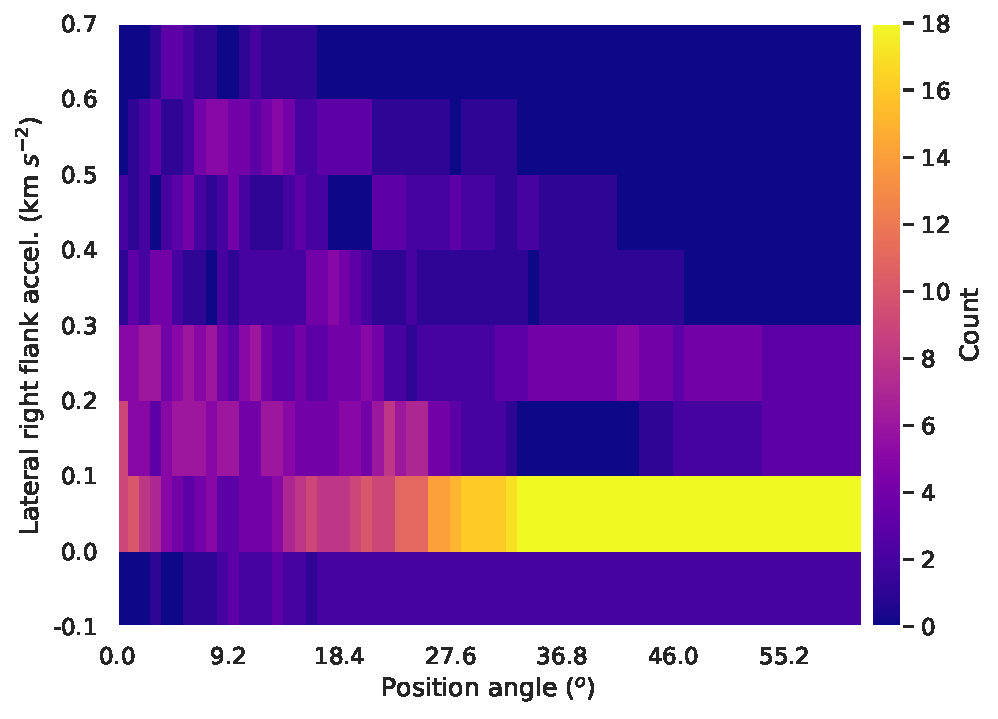
\includegraphics[width=0.32\textwidth,clip=]{chapter2/figs/latrightaccel_vs_latrightpos.pdf}
	}
	\centerline{
		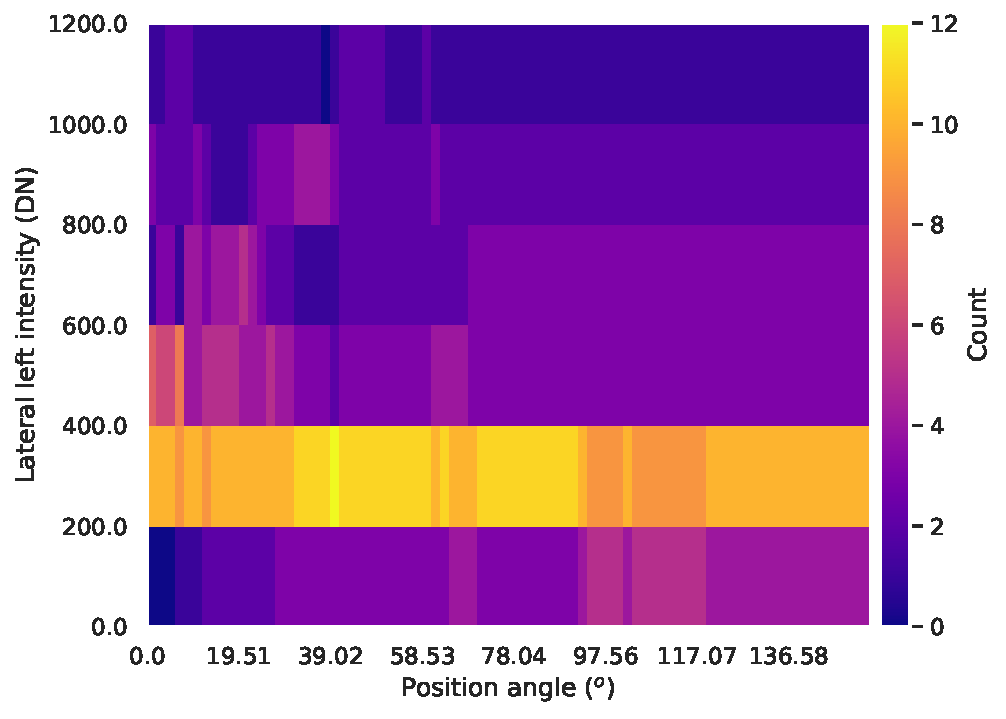
\includegraphics[width=0.32\textwidth,clip=]{chapter2/figs/latleftint_vs_latleftpos.pdf}
		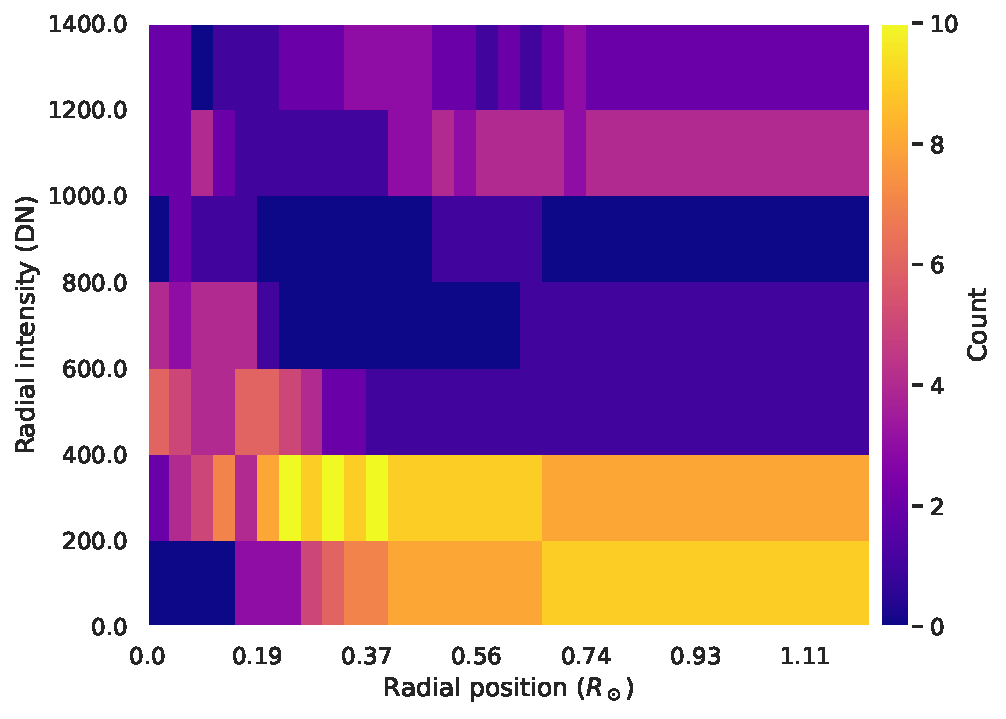
\includegraphics[width=0.32\textwidth,clip=]{chapter2/figs/radint_vs_radpos.pdf}
		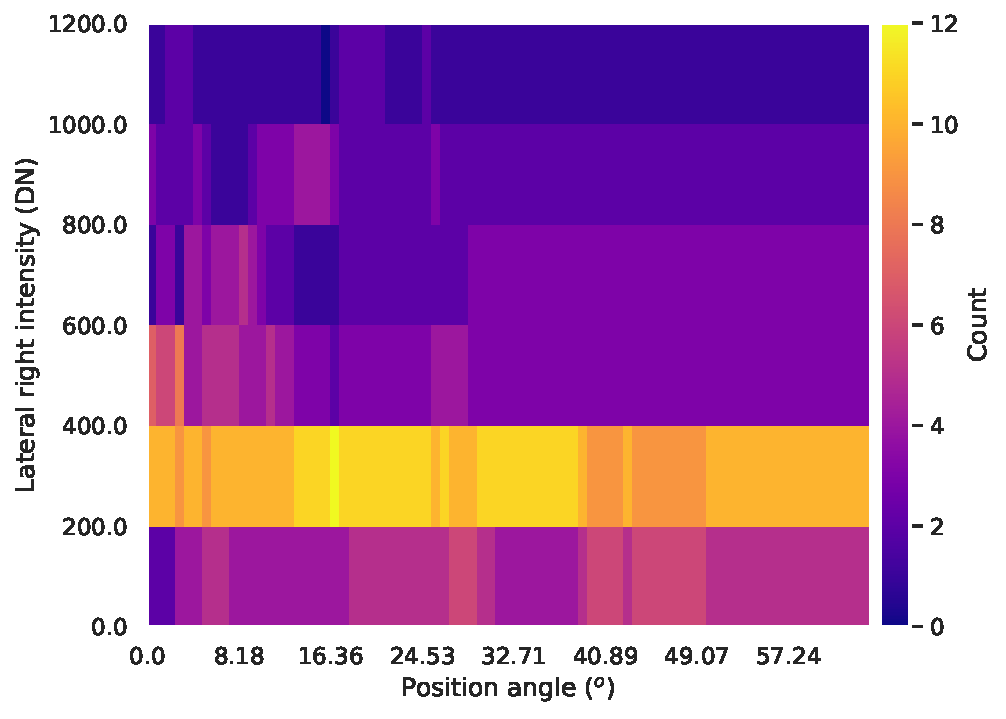
\includegraphics[width=0.32\textwidth,clip=]{chapter2/figs/latrightint_vs_latrightpos.pdf}
	}
	\centerline{
		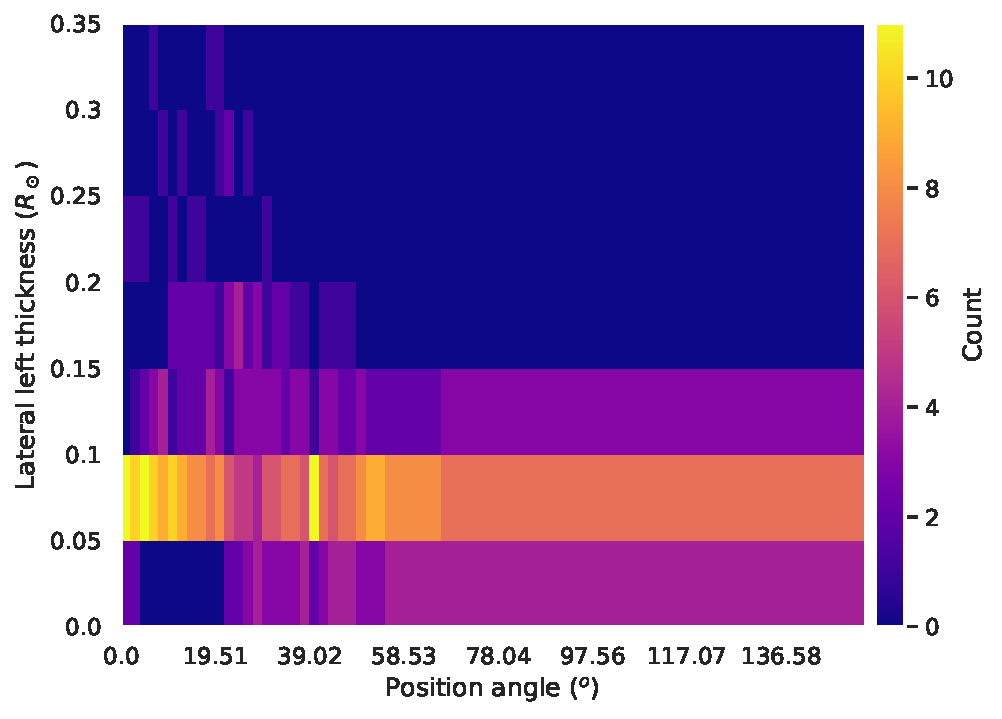
\includegraphics[width=0.32\textwidth,clip=]{chapter2/figs/latleftthick_vs_latleftpos.pdf}
		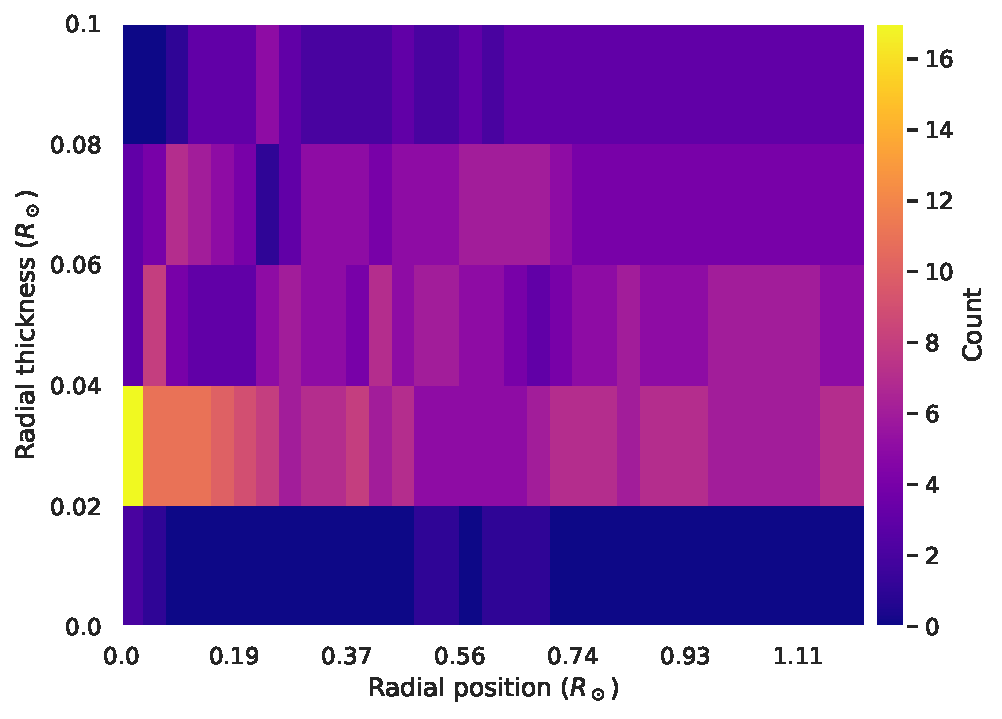
\includegraphics[width=0.32\textwidth,clip=]{chapter2/figs/radthick_vs_radpos.pdf}
		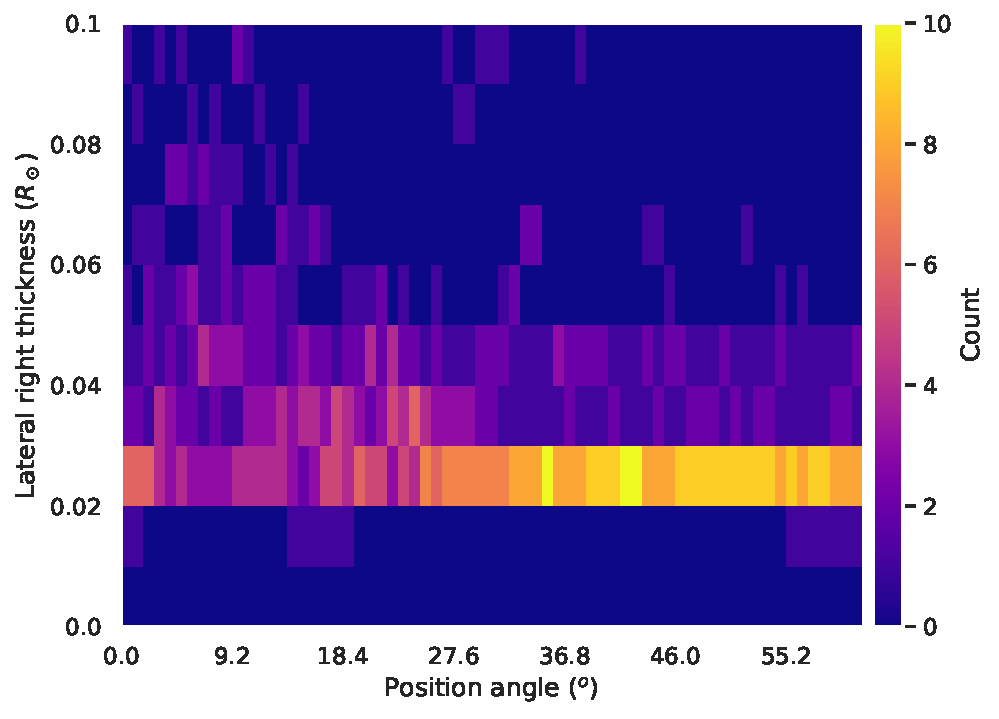
\includegraphics[width=0.32\textwidth,clip=]{chapter2/figs/latrightthick_vs_latrightpos.pdf}
	}
	\caption{Dynamic spectra of the EUV waves kinematics in the AIA FOV. The panels from the top to the bottom are the wave speeds, acceleration, mean intensity, and thickness. The left column is for the lateral left flank, the central column is for the radial direction, and the right column is for the lateral right flank.}
	\label{fig_kinematics_spect_hist}
\end{figure}

Histograms in Figure~\ref{fig_hist_plasma_param_corr} depict correlations between shock-field angle "\textit{THBN}", coronal magnetic field "\textit{BMAG}", plasma density "\textit{DENSITY}" Alfven speed "\textit{VA}", shock speed, and shock density jump "\textit{SHOCKJUMP}".
Moderate positive correlations exist between magnetic field and density, and between magnetic field and Alfven speed, suggesting common underlying physical processes.
A negative correlation between magnetic field and shock density jump implies stronger magnetic fields associate with smaller density jumps across shock surfaces, possibly due to magnetic field pressure resisting plasma compression or faster Alfven waves mitigating density jumps.
Further exploration is warranted to establish definitive connections and parameterize shock density jumps.

\begin{figure}[!htp] % updated!
	\centerline{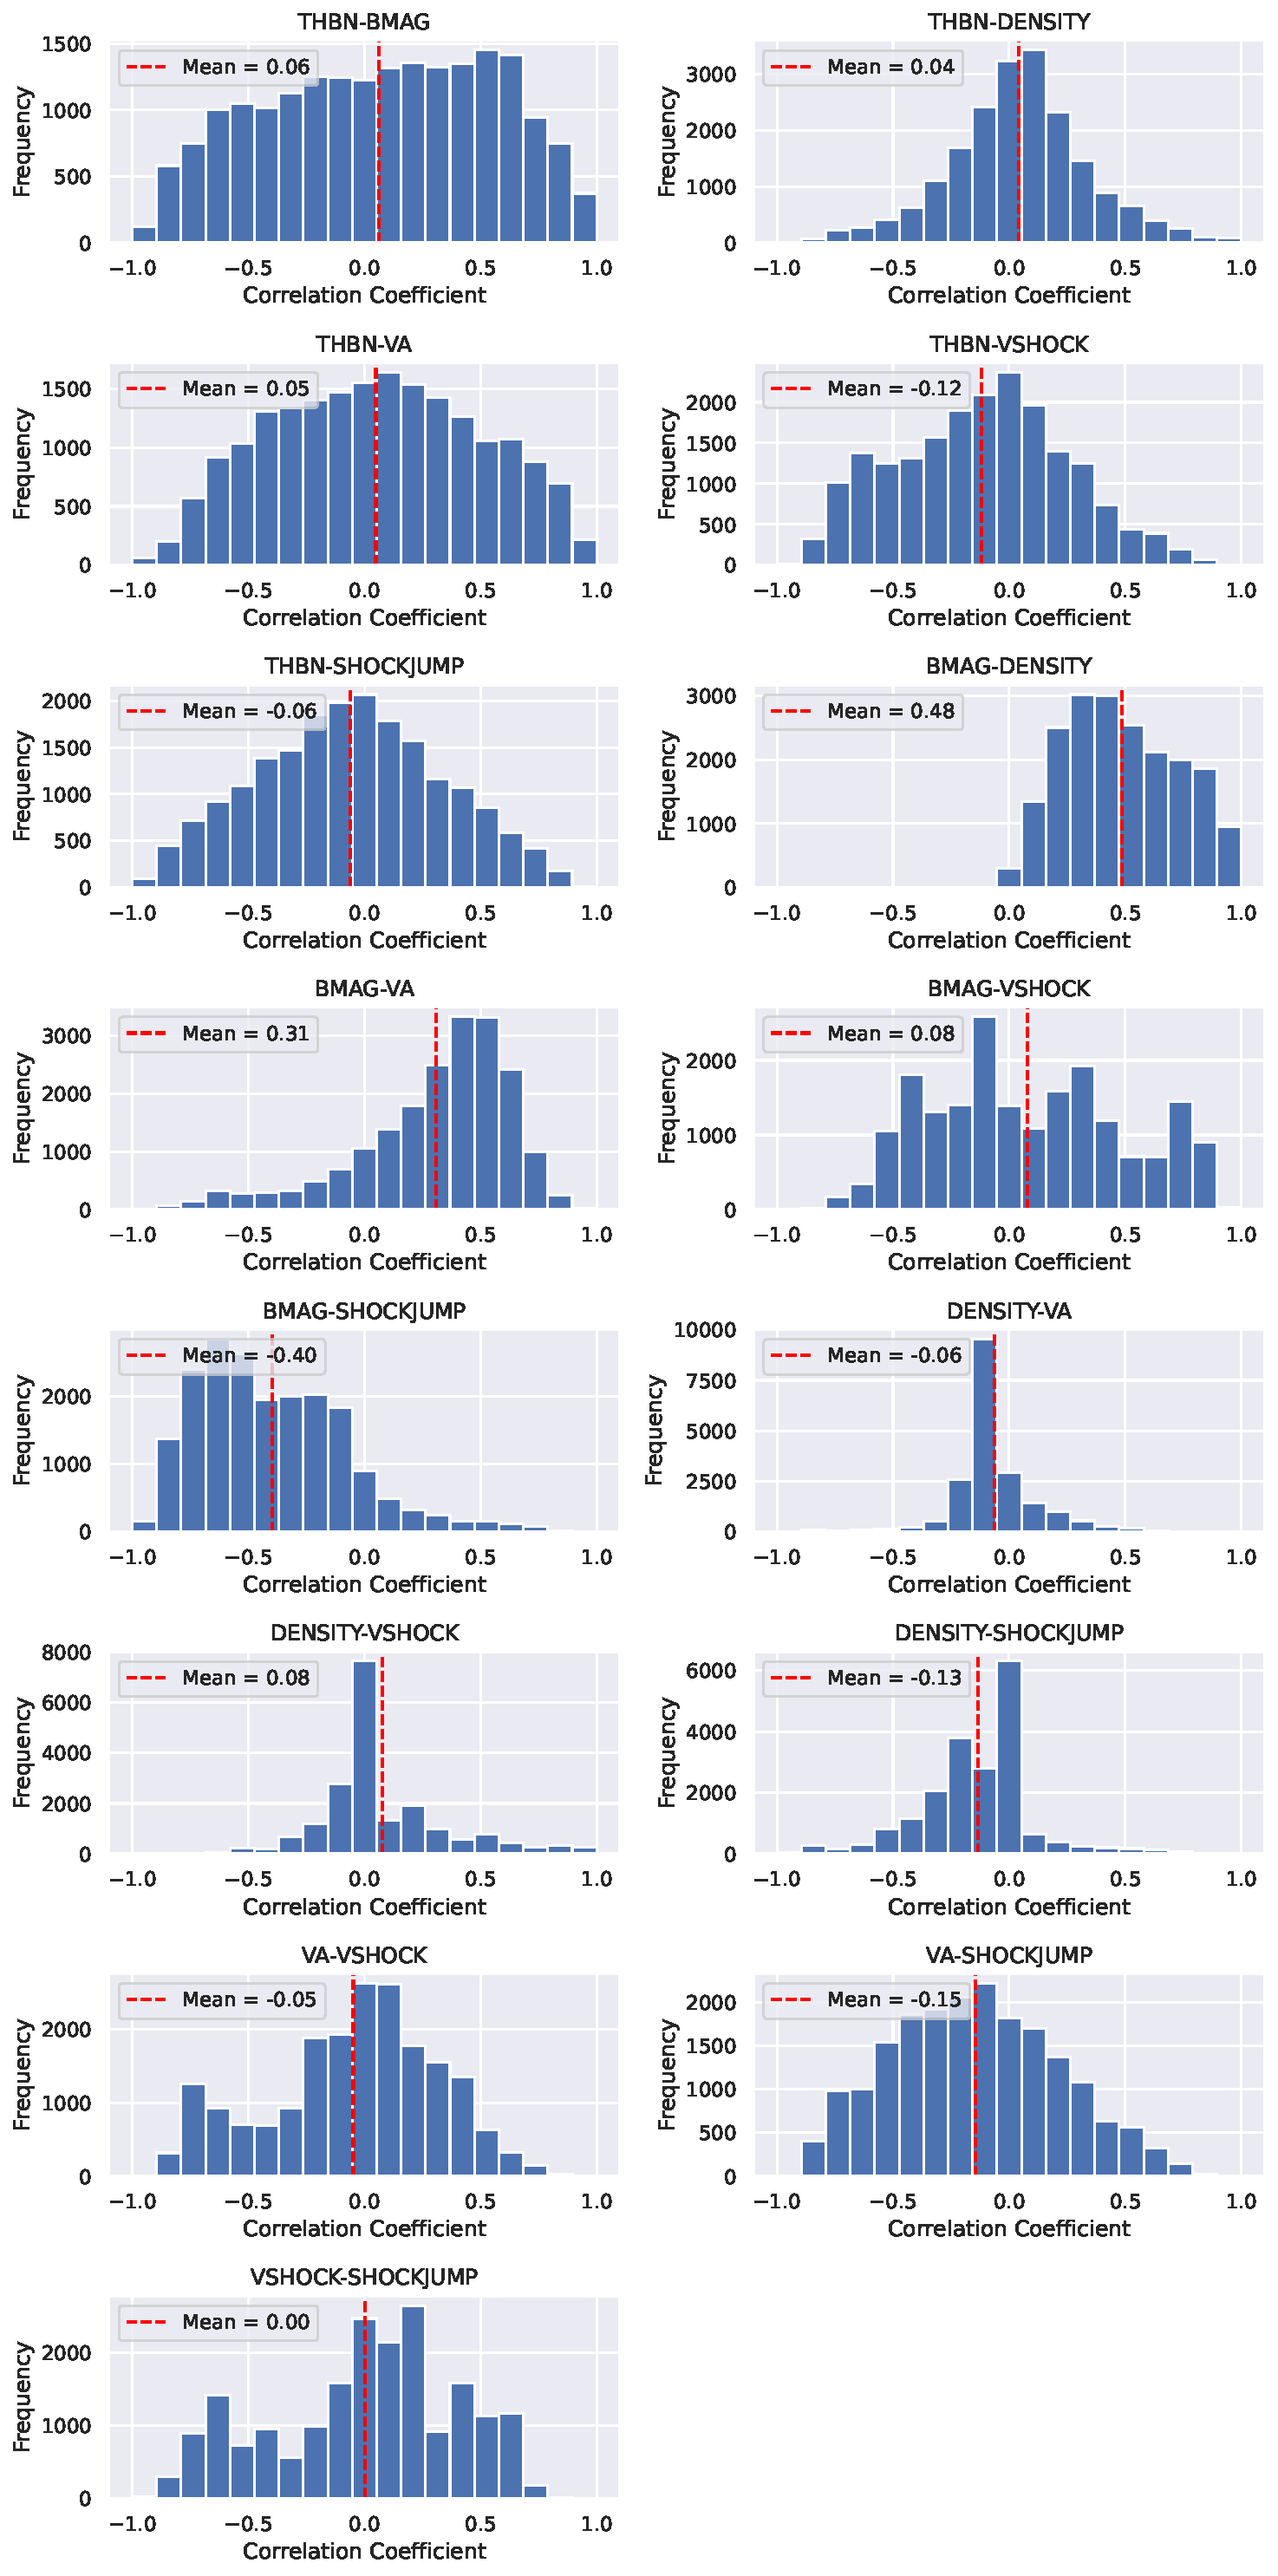
\includegraphics[width=0.7\columnwidth]{chapter2/figs/wp3_d2_Fig16.pdf}}
	\caption{Histograms of along-field-lines model plasma parameters in the solar corona for all the 26 events. The vertical dashed red lines are the mean values.}
	\label{fig_hist_plasma_param_corr}
\end{figure}

%%%%%%%%%%%%%%%%%%%%%%%%%%%%%%%%%%%%%%%%%%%%%%%%%%%%%%%%%%%%%%%%%%%%%%%%%%%%%%%%

\section{\textit{Wavetrack}: Automated Recognition and Tracking of Solar Eruptions}

\subsection{Overview}
The principal drivers of SEPs are acknowledged to be CME-driven shocks within the corona and interplanetary space. This acceleration primarily occurs through the diffusive shock acceleration (DSA) and shock drift acceleration (SDA) processes \citep{reames_2021}. Efforts have focused on characterizing SEP acceleration under ideal conditions \citep{vainio_2008, sokolov_2009, kozarev_2013}, with recent models incorporating observational data \citep{vourlidas_2012, kwon_2014, kozarev_2015, kozarev_2019}.

Understanding SEP acceleration requires comprehensive knowledge of CME-shock interactions with three-dimensional coronal fields \citep{rouillard_2016}. Modeling DSA necessitates deducing shock front shapes from observations, considering the impact of the local magnetic field-shock angle \citep{guo_2013}. EUV imaging, facilitated by instruments like STEREO \citep{wuelser_2004} and SDO/AIA \citep{lemen_2012}, enables shock characterization, supporting time-dependent modeling of SEP acceleration \citep{kozarev_2016, kozarev_2017, kozarev_2019}. Solar feature detection, including EUV waves, employs automated techniques \citep{aschwanden_2010, perez_Suarez_2011}, with challenges in wave recognition and tracking \citep{podladchikova_2005, verbeeck_2014, long_2014, ireland_2019}.

Wavetrack, a Python library, addresses these challenges by offering flexible solar feature detection and tracking \citep{stepanyuk_2022}. It integrates wavelet transforms and filtering, enabling multiscale data representation  \citep{starck_2002} and \'A trous wavelet transform \citep{akansu_1991, holschneider_1989}, essential for tasks like CME tracking.

Various techniques contribute to solar image analysis, including wavelet transform, image filtering, feature detection algorithms, machine learning, and solar feature tracking.

\begin{itemize}
	\item \textbf{Wavelet Transform}: The \'A trous wavelet transform facilitates multi-scale data representation, aiding feature extraction in solar image analysis.
	
	\item \textbf{Image Filtering}: Various techniques enhance specific features within solar images, aiding in phenomena detection.
	
	\item \textbf{Feature Detection Algorithms}: Automated algorithms improve solar feature identification efficiency across different observations.
	
	\item \textbf{Machine Learning}: Integration of machine learning techniques such as Convolutional Neural Networks (CNNs) and Generative Adversarial Networks (GANs) enriches solar image analysis capabilities.
	
	\item \textbf{Solar Feature Tracking}: Tracking algorithms monitor feature evolution over time, crucial for understanding solar processes.
\end{itemize}

Observations from SDO/AIA, particularly in 193 and 211 $\AA$ wavelengths, are instrumental in studying solar dynamic features, facilitating CBF analysis and tracking.

\subsection{Image Filtering Techniques}
Image filtering techniques, including thresholding, wavelet decomposition, and segmentation, were central to the method. Initial thresholding narrowed the dynamic range of base difference images, focusing on the object of interest.

Following thresholding, the base difference images underwent \'A trous wavelet decomposition into multiple scales. Each wavelet coefficient was then thresholded relative to the statistical distribution of pixel intensities at each decomposition level. Segmentation produced object masks for each time step, which were subsequently multiplied by the original data to reveal intensity variations within the object.

Tailored approaches were employed due to variations in statistical distributions of pixel intensities between base and running difference images. Base difference images focused on specific segments containing the object of interest, such as a CBF, while running difference images, used for eruption initiation identification, were dependent on specific features and objects observed.

The \'A trous wavelet transform, providing a multi-scale data representation, significantly contributed to solar image recognition and tracking. This hierarchical decomposition facilitated the extraction of specific objects and their masks from imaging observations, aiding in their tracking and temporal analysis. It enhanced the visibility of faint features like EUV waves, offering a versatile framework applicable to various solar phenomena across different wavelengths, thus serving as a valuable tool for analyzing CME shock waves and filaments.

The study introduced the Wavetrack package, an automated tool for detecting and tracking dynamic coronal features in solar observations. By utilizing wavelet decomposition, feature enhancement, filtering, and object recomposition, Wavetrack identified and tracked features such as CBFs and eruptive filaments. This Python framework, adaptable to both on-disk and off-limb features, facilitates tracking of features evolving over time.

\subsection{Wavetrack for Coronal Wave and Filament Tracking}
Wavetrack employed wavelet decomposition, feature enhancement, and filtering for tracking coronal waves. The method enhanced faint features like EUV waves using the \'A trous wavelet decomposition. Automated feature recognition, including intensity thresholding and segmentation, isolated coronal wave features, generating time-dependent pixel masks for both on-disk and off-limb features.

For filament tracking, Wavetrack utilized wavelet decomposition, feature recognition, object mask generation, and image recomposition. The method identified different scales of features and enhanced them for tracking. Object masks isolated filament features at each time step, and image recomposition produced final feature maps. Image choice, such as inverted AIA 193 $\AA$ images, depended on source data and filament velocity.

\subsection{Fourier Local Correlation Tracking (FLCT) Model}
The study employed the FLCT model to determine solar feature velocities, utilizing the FLCT method. FLCT analyzed consecutive solar images and tracked feature motion over time using object masks from Wavetrack. The output provided detailed maps of instantaneous velocity, aiding in understanding solar feature expansion and evolution.

The study integrated advanced image processing techniques, including wavelet transform, filtering, feature detection algorithms, and machine learning, for comprehensive solar observation analysis. Wavetrack emerged as a versatile tool, particularly valuable for dynamic coronal feature tracking, offering significant insights into solar dynamics.

\subsection{Results}
The study showcases the versatility of the Wavetrack package through several examples:

\begin{enumerate}
	\item \textbf{May 11, 2011 event}:
	Wavetrack algorithm tracked an erupting filament and its associated coronal bright front (CBF), revealing their relationship using AIA 193 $\AA$ observations.
	
	\item \textbf{September 29, 2013 event}: Wavetrack monitored a large-scale filament eruption, consistently tracking features on the solar disk and corona.
	
	\item \textbf{December 12, 2013 event}: Wavetrack analyzed driven and non-driven regions of a CBF, revealing its relation to eruptive features.
	
	\item \textbf{June 07, 2011 event}: Wavetrack observed significant radial speed variations and stable angle changes during a compressive front event.
\end{enumerate}

\begin{figure}[!htp]
	\centering
	\includegraphics[width=0.7\hsize]{chapter2/figs/wavetrack_figure_110511.png}
	\caption{Wavetrack images of a May 11, 2011 eruption, with CBF mask applied. Four image pairs shown, separated by 2 minutes, to track CBF over time. Credit goes to \citet{stepanyuk_2022}.}
	\label{fig_wavetrack_cbf_center}
\end{figure}

Focusing on the May 11, 2011 event accompanied by a CBF, the methodology was applied to three events observed by AIA \citep{kozarev_2015, kozarev_2017}. Wavetrack adeptly tracked CBF evolution both on the solar disk and off the limb, maintaining performance despite pixel distribution and intensity differences.
The application facilitated detailed study of CBF shapes and intensity distributions, separate from the broader corona. Wavetrack effectively segmented CBF objects under different activity states, highlighting its capability to track multiple separate parts of the same feature.

Wavetrack was used to isolate and study CBF and filament kinematics using the FLCT method. Figure~\ref{fig_wavetrack_cbf_center} shows FLCT results of the May 11, 2011 event, revealing uneven expansion of the CBF from the central source. The combined approach elucidated dynamic behavior not discernible from intensity observations alone.
Figure~\ref{fig_flct_110511} displays the direction and speed of each CBF region. It reveals uneven expansion, with the thinnest part, strongly driven by the erupting filament, moving fastest. This nuanced insight, inaccessible through intensity observations alone, highlights the value of our combined Wavetrack and FLCT approach in understanding coronal feature dynamics.
Figure~\ref{fig_wavetrack_center_of_mass} depicts thorough analysis of CBF centers of mass (CM) and geometric centers (GC), illustrating their positional and speed variations over time. These findings provide valuable insights into CBF dynamics during the specified event.

\begin{figure}[!htp]
	\centering
	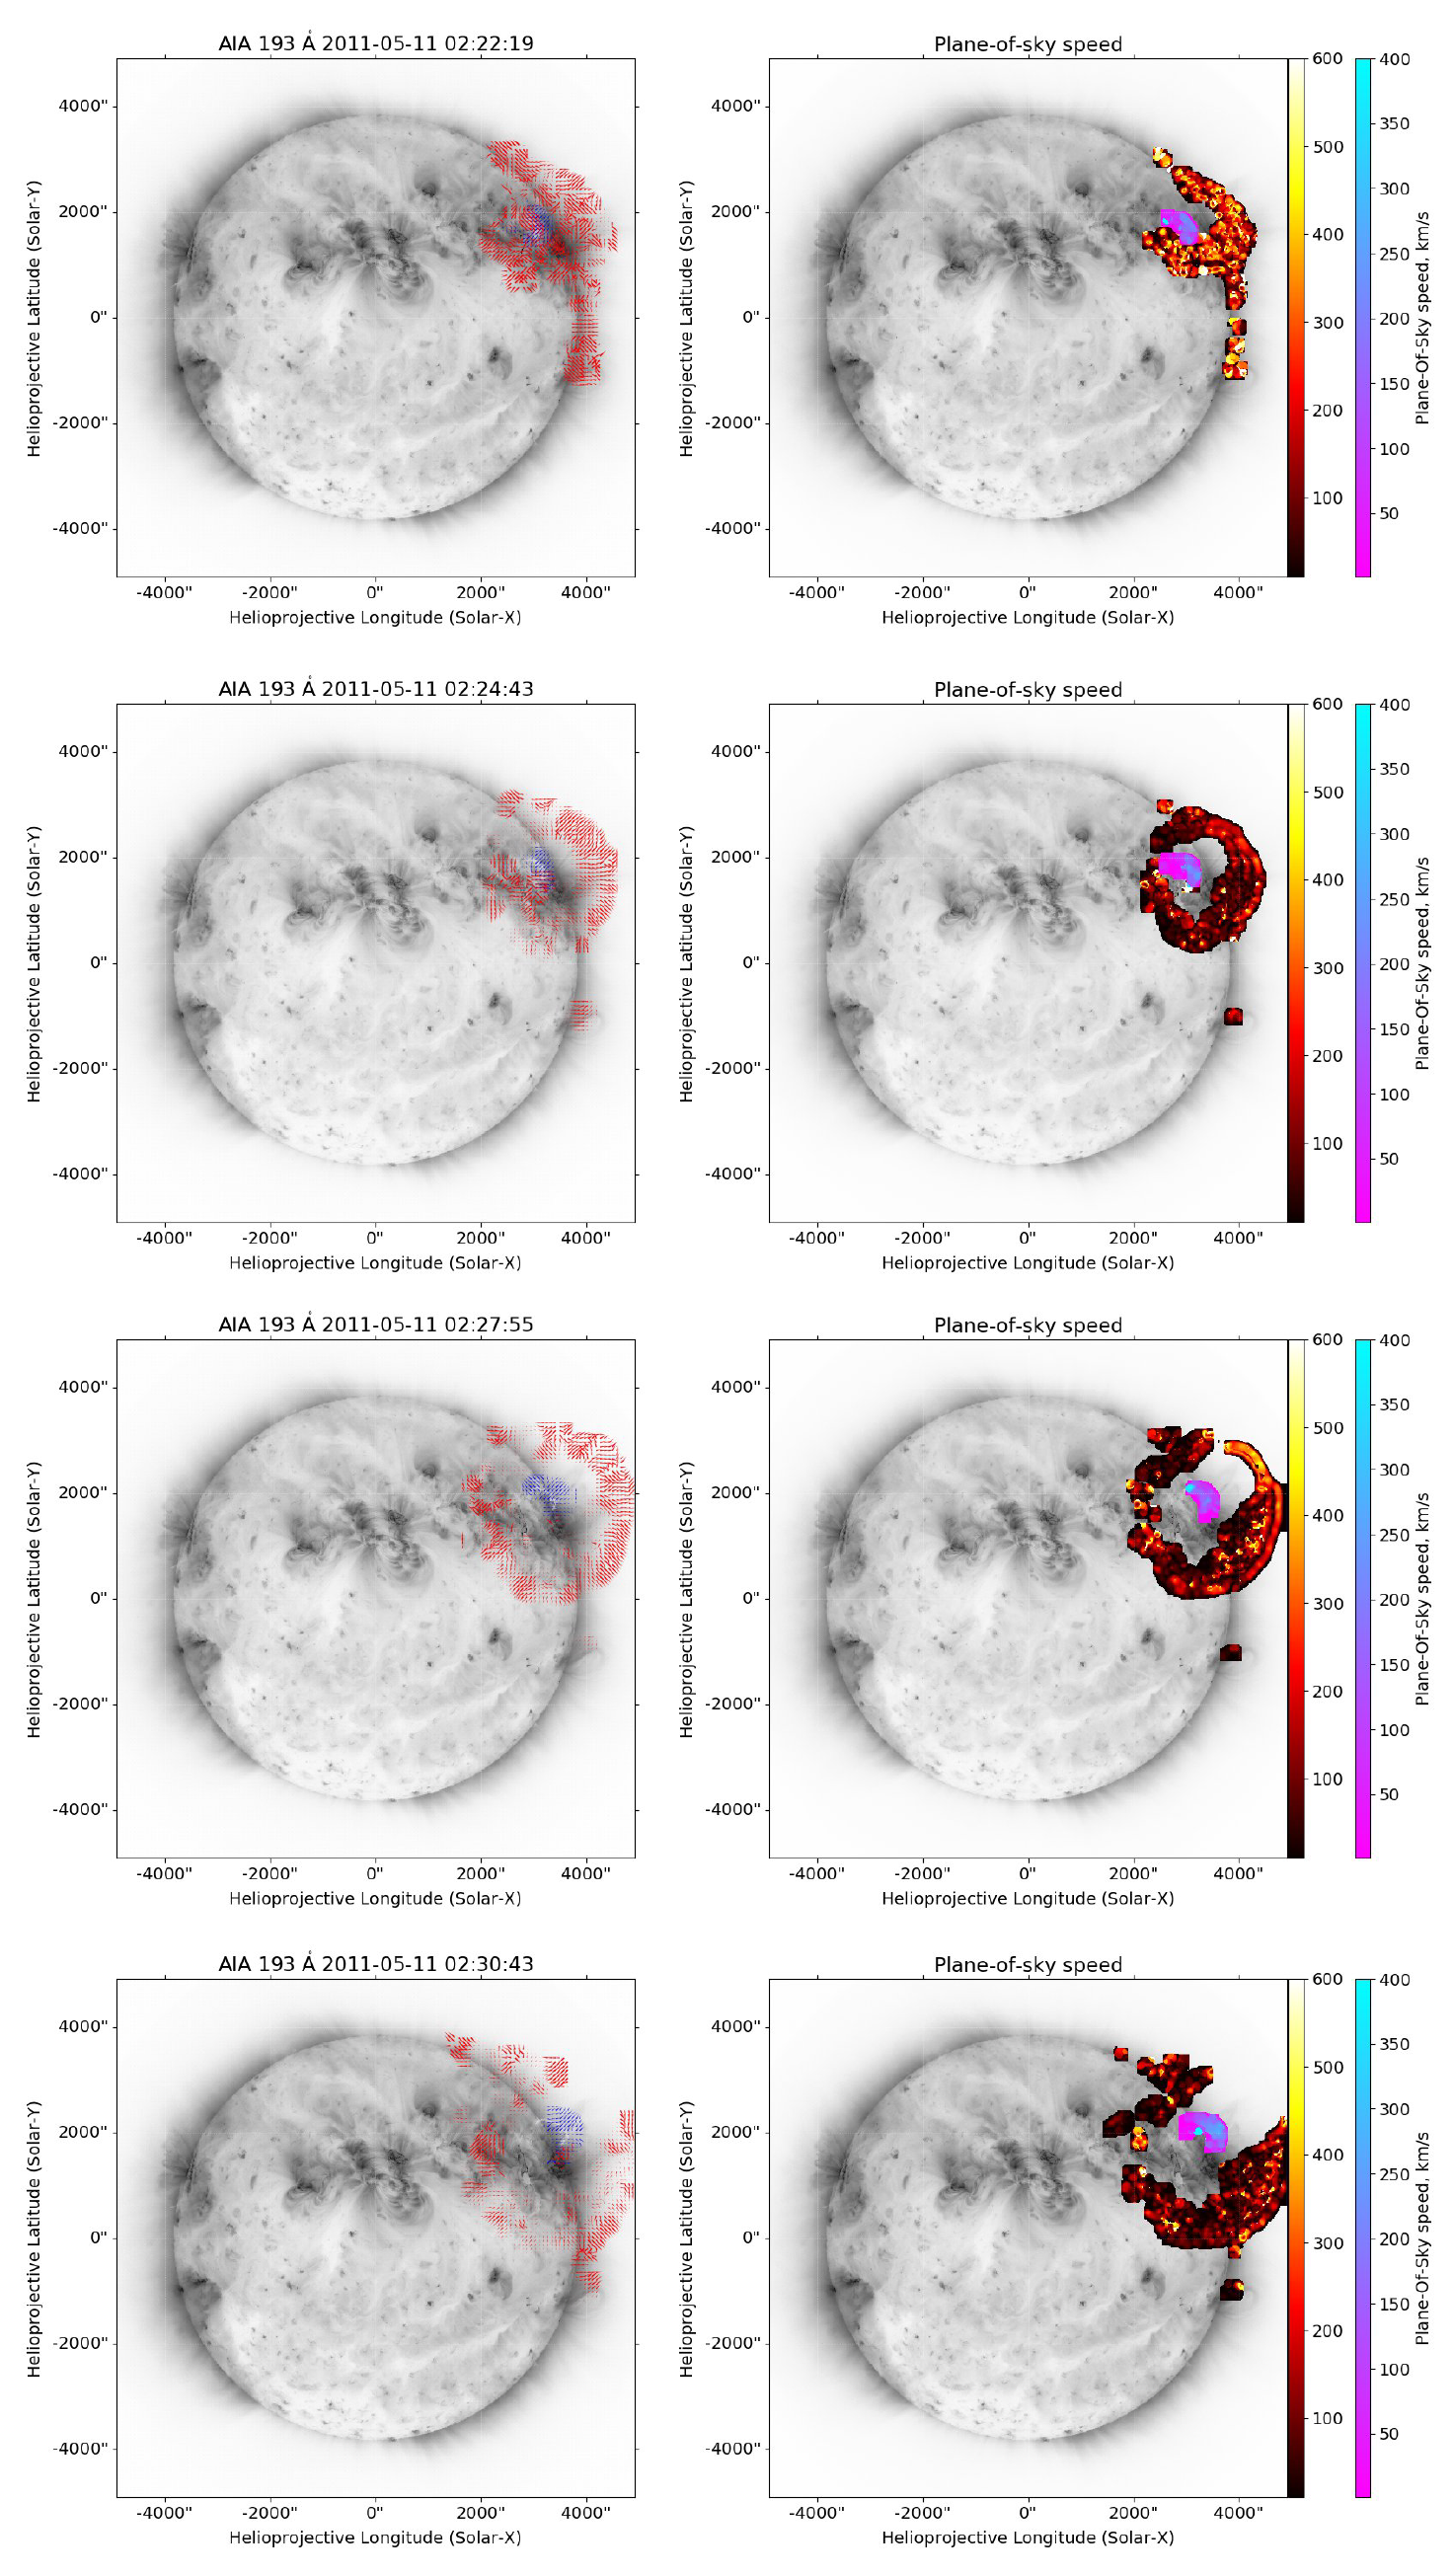
\includegraphics[width=0.7\hsize]{chapter2/figs/flct_wave_filament_doubleplot_figure_110511.png}
	\caption{FLCT model output for four image pairs from Fig. 3. Left: the plane-of-sky velocity vectors. Right: plane-of-sky speed. Credit goes to \citet{stepanyuk_2022}.}
	\label{fig_flct_110511}
\end{figure}

\begin{figure}[!htp]
	\centering
	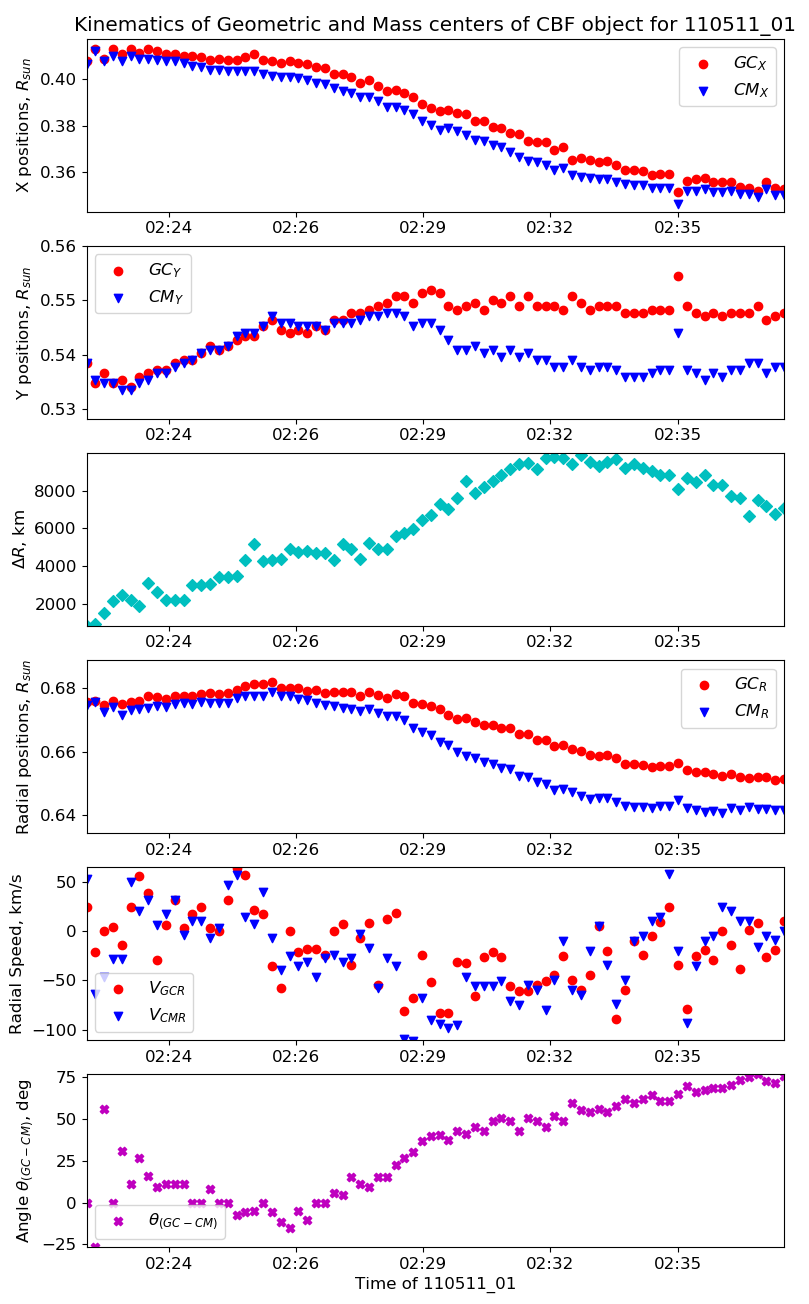
\includegraphics[width=0.7\hsize]{chapter2/figs/event_110511_01_centers_of_mass.png}
	\caption{Analysis of the center of mass and geometric centers' motion during the May 11, 2011 event. The different rows present the X-, Y-, and R- positions for both GC and CM, the distance between GC and CM in \textit{km}, and the angle between these two points over time. Credit goes to \citet{stepanyuk_2022}.}
	\label{fig_wavetrack_center_of_mass}
\end{figure}

%%%%%%%%%%%%%%%%%%%%%%%%%%%%%%%%%%%%%%%%%%%%%%%%%%%%%%%%%%%%%%%%%%%%%%%%%%%%%%%%

\section{Geomagnetic Storms: CME Speed De-Projection vs. In Situ Analysis}
This study, led by \citet{miteva_2023}, examines the relationship between geomagnetic storm (GS) intensity and solar/interplanetary phenomena. Using the \textit{PyThea} framework, we reconstruct 3D geometry of geo-effective CMEs and compare on-sky and de-projected speed values, employing spheroid, ellipsoid, and graduated cylindrical shell (GCS) models. We investigate parameters of GS-associated phenomena, finding that fast CME speeds combined with specific magnetic structure orientations are indicative of GS strength. Accurate estimations of geometry, direction, and de-projected speeds are crucial for GS forecasting in space weather prediction schemes.

\subsection{Overview}
Solar eruptive events such as CMEs and solar flares (SFs) influence space weather, with electromagnetic radiation preceding energetic particles and CME plasma clouds \citep{fletcher_2011, webb_2012, klein_2017, temmer_2021, malandraki_2018, gopalswamy_sun_sw_2022}. Geomagnetic storms (GSs) occur due to interactions between solar wind plasma and Earth's magnetosphere, facilitated by magnetic reconnection during events like CME impacts \citep{dungey_1961, akasofu_1981, echer_2022, gonzalez_1994, saiz_2013, lakhina_2016}. Fast CMEs cause intense GSs, affecting technology and inducing disruptions in near-Earth space \citep{tsurutani_1997, zhang_2007, wu_2016, borovsky_2006, pulkkinen_2007}.

However, single spacecraft observations limit accurate CME speed estimations due to projection effects \citep{paouris_2021, kouloumvakos_2022}. Previous studies found no clear correlation between GS intensity and solar flare/CME parameters \citep{samwel_2023}, highlighting the need for reliable early warnings based on solar or near-Sun measurements. Accurate prediction of CME impact on Earth requires understanding their directionality and geometry, crucial for maximizing forecast lead time \citep{kay_2018, vourlidas_2003, jackson_2010}.

Improving reconstruction techniques to correct projection effects enhances CME propagation understanding and forecasting \citep{thernisien_2009, mierla_2010, wood_2010, thernisien_2011}. Existing CME propagation models exhibit discrepancies between 2D and 3D speeds and widths \citep{odstrcil_2004, xie_2004, vrvsnak_2013, pomoell_2018, jang_2016, verbeke_2022}. This study focuses on deducing CME directionality and near-Sun speeds using the PyThea framework \citep{kouloumvakos_2022}, analyzing geo-effective cycle 24 CMEs and their correlations with GS intensity and interplanetary parameters.

The event selection process identified 25 significant GSs within Solar Cycle 24 (SC24) and associated them with potential IP and/or solar phenomena. This involved temporal associations with IP and ICME events, CMEs, and solar flares. Various databases and catalogs were utilized for this analysis \citep{gonzalez_1994, gopalswamy_gs_2022, qiu_2022, besliu_2022, abe_2023, zhang_2007, gonzalez_2007, gopalswamy_2008, echer_2013, manu_2022}.

Utilized databases and catalogs include the GS database Kyoto\footnote{\url{https://wdc.kugi.kyoto-u.ac.jp/dstdir/index.html}}, SF database (GOES)\footnote{\url{http://ftp.swpc.noaa.gov/pub/warehouse/}}, CME catalog (SOHO-LASCO)\footnote{LASCO CME Catalog: \url{https://cdaw.gsfc.nasa.gov/CME_list/}}, ICME Wind and ACE databases\footnote{\url{https://wind.nasa.gov/ICME_catalog/ICME_catalog_viewer.php}},\footnote{\url{https://izw1.caltech.edu/ACE/ASC/DATA/level3/icmetable2.htm}}, and IP shock database (Wind)\footnote{\url{http://www.ipshocks.fi/database}},\footnote{\url{https://lweb.cfa.harvard.edu/shocks/wi_data/}}. These resources were accessed for relevant data retrieval and analysis \citep{selvakumaran_2016}.

\subsection{PyThea 3D De-Projection Tool}
This investigation employs the PyThea online tool for 3D reconstruction of CMEs and shock waves \citep{kouloumvakos_2022}, utilizing spheroid, ellipsoid, and GCS models. Two independent observers conduct fitting procedures. Figure~\ref{fig_3D_fit} illustrates fits for event E03, revealing observer bias in structure alignment with the model, potentially leading to CME width overestimation. However, despite this bias, overall results for event E03, including directivity and speed, remain minimally impacted, though discrepancies may arise among different observers.

\begin{figure}[!htp]
	\centering
	\begin{subfigure}[b]{0.3\textwidth}
		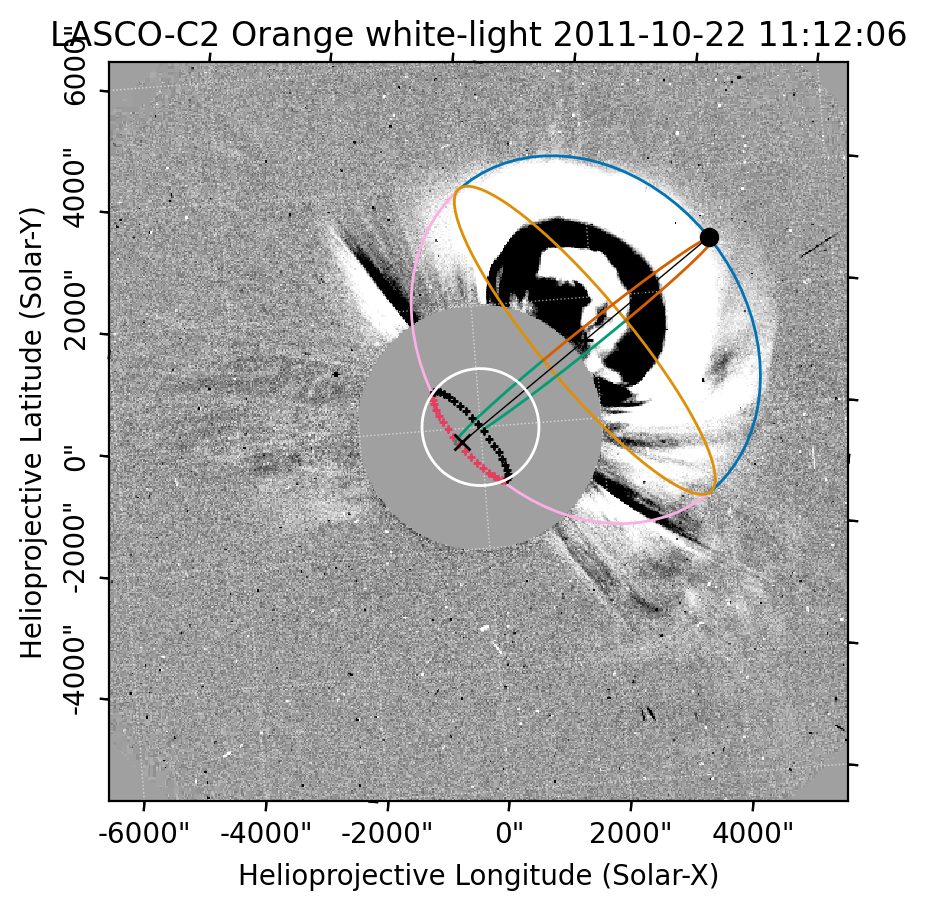
\includegraphics[width=\textwidth]{chapter2/figs/Fig_s1.png}
	\end{subfigure}
	\hfill
	\begin{subfigure}[b]{0.3\textwidth}
		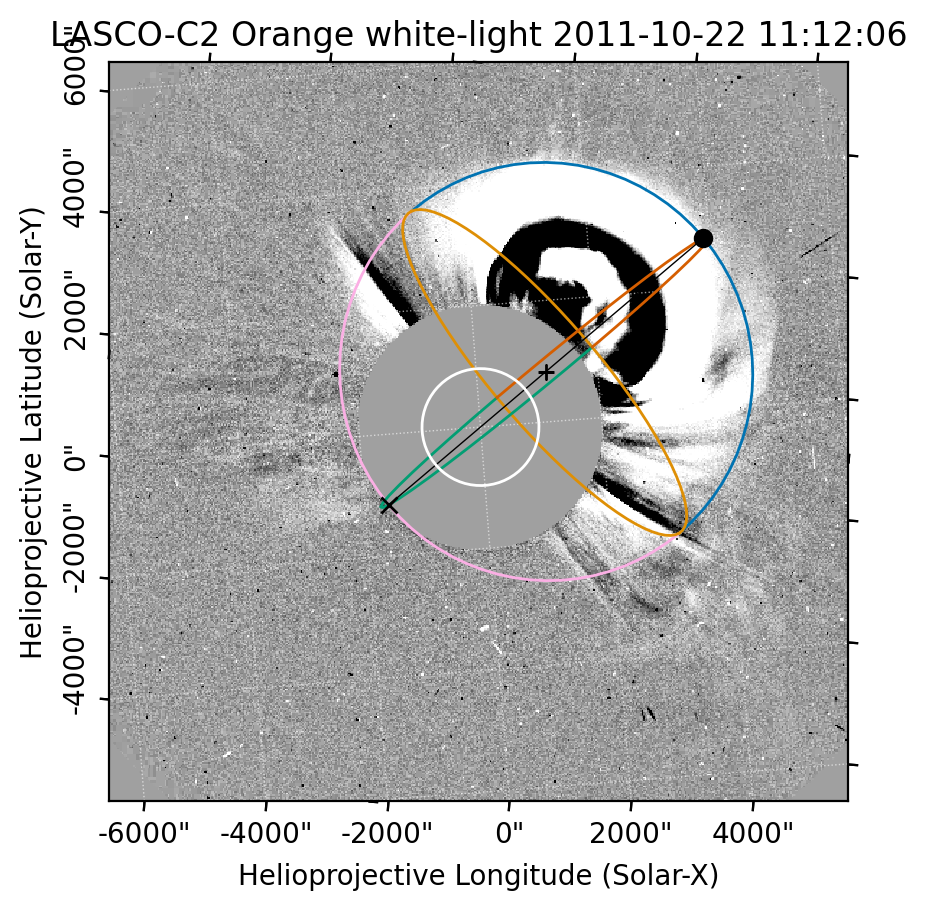
\includegraphics[width=\textwidth]{chapter2/figs/Fig_e1.png}
	\end{subfigure}
	\hfill
	\begin{subfigure}[b]{0.3\textwidth}
		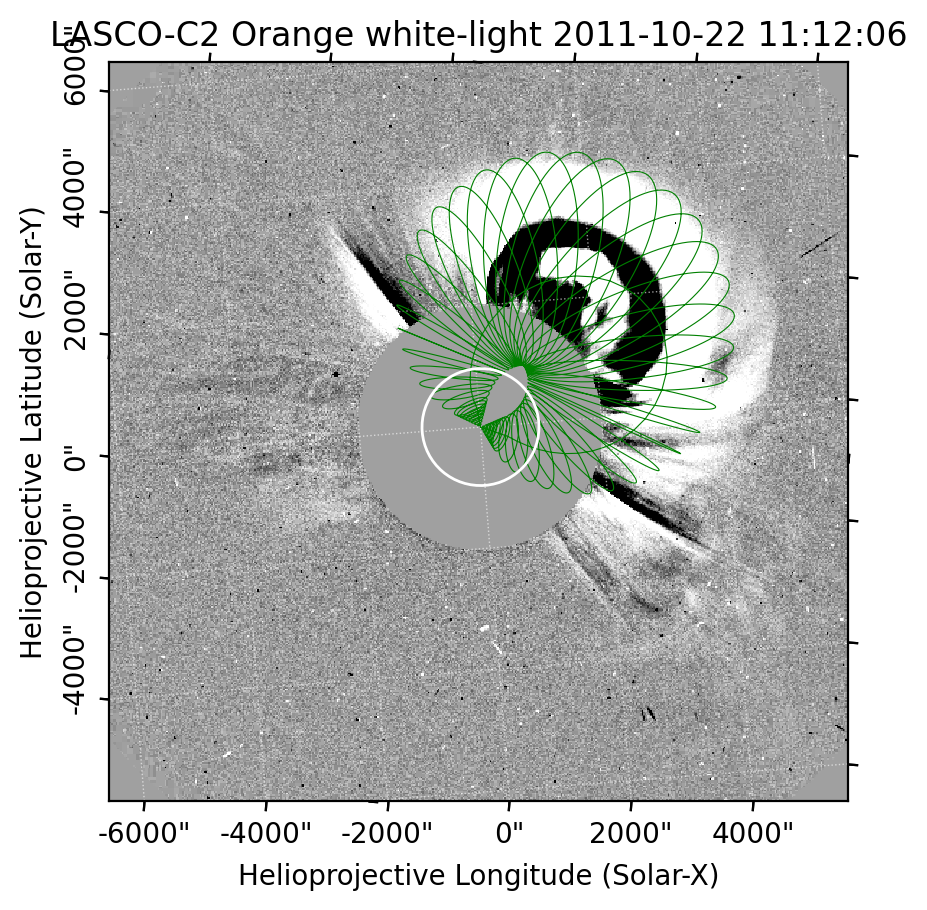
\includegraphics[width=\textwidth]{chapter2/figs/Fig_g1.png}
	\end{subfigure}
	\medskip % Add some vertical space between rows
	\begin{subfigure}[b]{0.3\textwidth}
		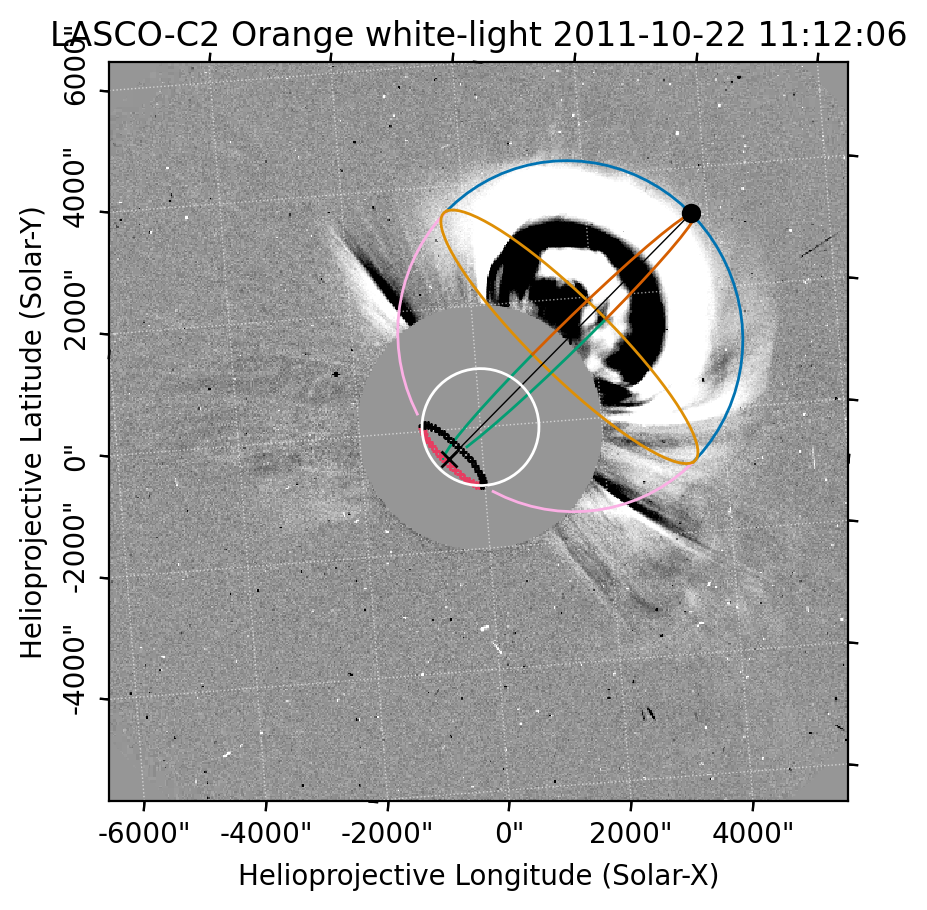
\includegraphics[width=\textwidth]{chapter2/figs/Fig_s2.png}
	\end{subfigure}
	\hfill
	\begin{subfigure}[b]{0.3\textwidth}
		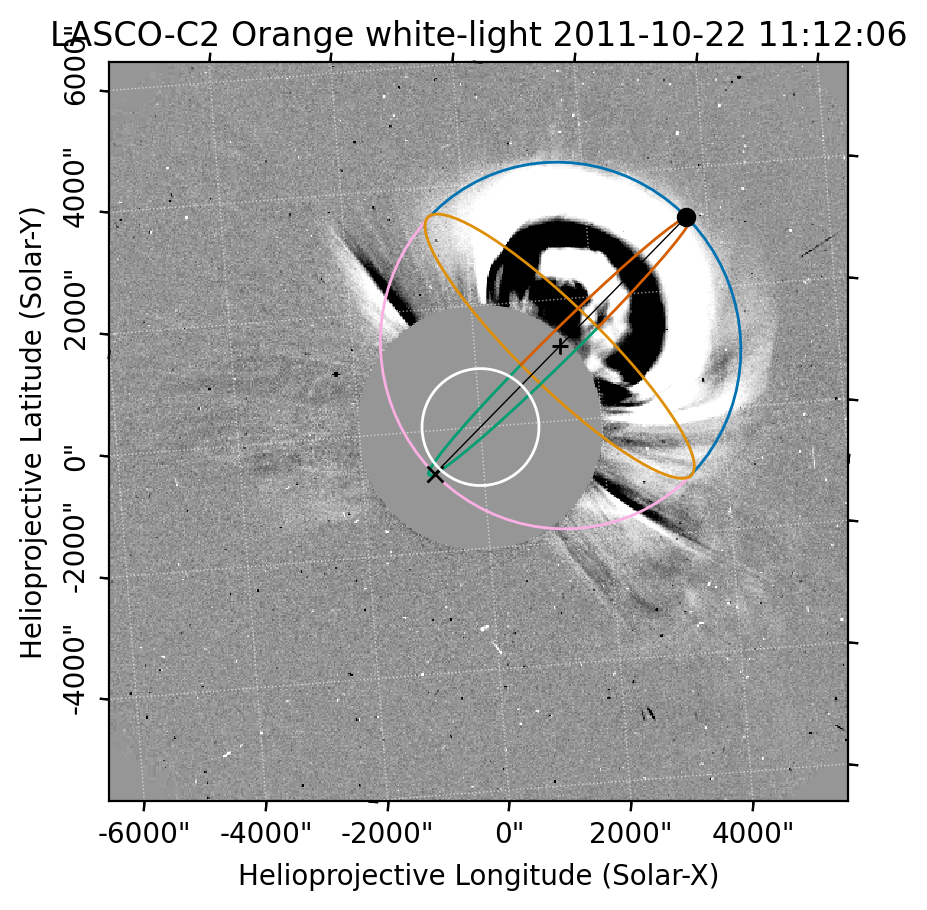
\includegraphics[width=\textwidth]{chapter2/figs/Fig_e2.png}
	\end{subfigure}
	\hfill
	\begin{subfigure}[b]{0.3\textwidth}
		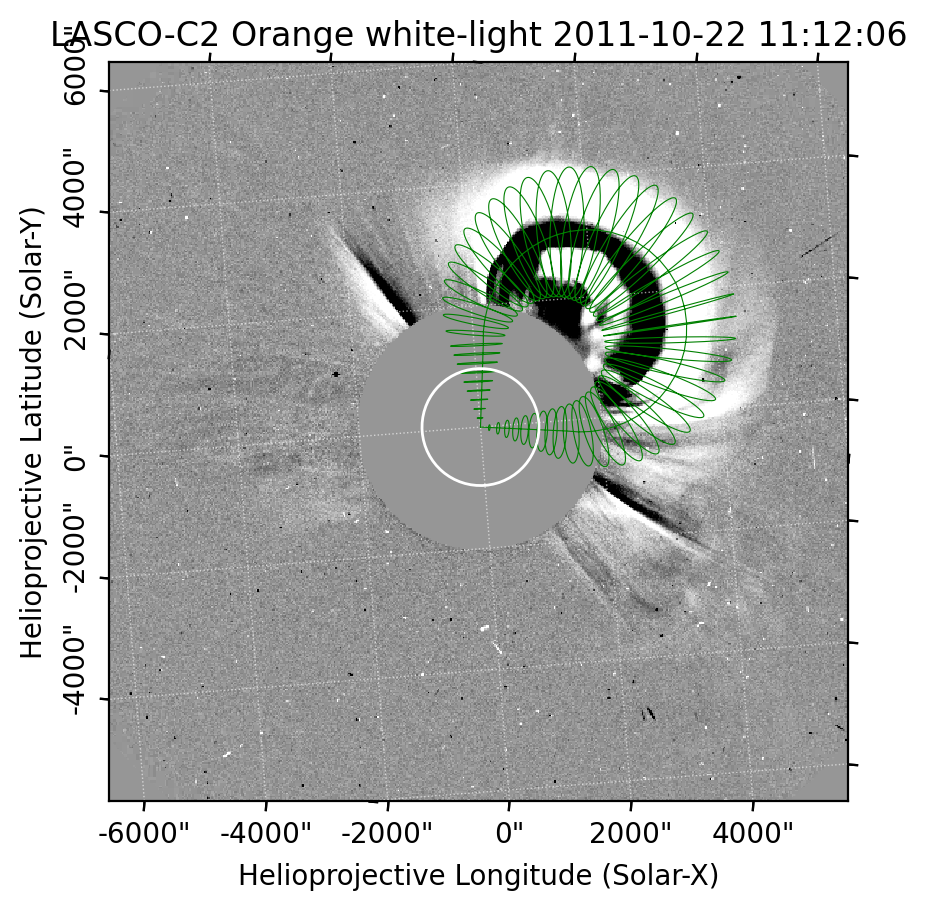
\includegraphics[width=\textwidth]{chapter2/figs/Fig_g2.png}
	\end{subfigure}
	\caption{3D reconstructions of a CME (E03) using the spheroid, ellipsoid, and GCS model from the PyThea tool performed by observers 1 and 2 (top and bottom row, respectively). Credit goes to \citet{miteva_2023}.}
	\label{fig_3D_fit}
\end{figure}

In five cases (E05, E11, E17, E18, E22), attempts to identify SFs or CMEs were unsuccessful, while in six additional cases, SF specifications were unattainable. Events with uncertain CME origins were excluded from subsequent 3D analyses. For example, the unique orientation of a double CME in case E07 rendered its de-projection unfeasible, leading to its exclusion. Similarly, in seven cases (E12, E14–E16, E19, E23, E25), data retrieval issues from both spacecraft led to their omission from 3D analyses.

The study focuses on deriving de-projected CME speeds based on fits at two distinct time steps. Initial CME longitude and latitude are manually specified for each model, utilizing provided SF locations. Final CME directivity is considered relatively crude, derived from qualitative information extracted from available animations\footnote{\helioweatherurl}. This approach ensures a rigorous basis for evaluating de-projected CME speeds.

\subsection{Results}
\subsubsection{Projection Effects}
Approximately 10 CMEs were analyzed by two designated observers in our research team, including myself, utilizing all three models in the PyThea framework. The fitting process involved two time steps to derive velocity parameters based on height–time estimations. Both observers conducted the 3D de-projection procedure iteratively for each event, resulting in averaged CME speeds presented in Table~\ref{tab_fits}, rounded to the nearest tenth. Discrepancies between fitting instances were treated as errors, ranging from 10 \kms to twice the estimated speed. Figure~\ref{fig_vcme_err} illustrates the correlation between 3D speeds and estimated errors, showing significant variability, particularly with the GCS model, but a discernible positive trend between error magnitude and CME speed.

Subjectivity and varied experience levels among observers influenced the visual fitting process, leading to differences in evaluated speeds, both within individual observers using the same model and across different models for a single observer. Variations in operating system software also contributed to result discrepancies. Events E04, E08, and E21 were incomplete due to PyThea computing issues or substantial uncertainty in CME structure assessment.

Our findings highlight the inherent subjectivity in procedures relying on personal judgment for fit quality, detailed further in \citep{verbeke_2022}. Averaged CME speeds, meticulously outlined in Table~\ref{tab_fits}, will serve as the basis for subsequent correlation studies.

\begin{table}[!htp]
	\caption{CME Speeds (\kms) for Observers 1 and 2. Credit goes to \citet{miteva_2023}.}
	\label{tab_fits}
	\centering
	\begin{tabular}{ccccccc}
		\toprule
		\textbf{\#} & \multicolumn{2}{c}{\textbf{Spheroid}} & \multicolumn{2}{c}{\textbf{Ellipsoid}} & \multicolumn{2}{c}{\textbf{GCS}} \\
		& \textbf{obs1} & \textbf{obs2} & \textbf{obs1} & \textbf{obs2} & \textbf{obs1} & \textbf{obs2} \\
		\midrule
		E01 & $2170\pm870$ & $1800\pm270$ & $2130\pm200$ & $1710\pm450$ & $1590\pm100$ & $1760\pm10$ \\
		E02 & $1780\pm140$ & $1350\pm50$  & $1880\pm580$ & $1310\pm90$ & $1780\pm260$ & $1630\pm130$ \\
		E03 & $770\pm40$ & $740\pm10$ & $640\pm180$ & $740\pm180$ & $1020\pm170$ & $700\pm270$ \\
		E04 & - & $2150\pm140$ & - & $2460\pm70$ & - & $2530\pm630$ \\
		E06 & $1410\pm420$ & $710\pm70$ & $1870\pm50$ & $1700\pm300$ & $1680\pm870$ & $1560\pm470$ \\
		E08 & $350\pm90$ & - & $360\pm150$  & - & $350\pm70$ & - \\
		E09 & $690\pm280$ & $630\pm150$ & $550\pm170$  & $590\pm60$ & $670\pm610$ & $710\pm220$ \\
		E10 & $840\pm380$ & $610\pm1040$ & $1120\pm360$ & $960\pm90$ & $1160\pm650$ & $1310\pm80$ \\
		E13 & $320\pm90$ & $350\pm50$ & $620\pm140$ & $750\pm160$ & $780\pm80$ & $1310\pm700$ \\
		E20 & $830\pm190$ & $800\pm600$ & $790\pm90$ & $570\pm20$ & $1240\pm280$ & $1130\pm230$ \\
		E21 & $620\pm230$ & - & $440\pm40$ & - & $280\pm180$ & - \\
		E24 & $750\pm270$ & $1310\pm220$ & $880\pm350$ & $2020\pm960$ & $950\pm120$ & $1560\pm540$ \\
		\bottomrule
	\end{tabular}
\end{table}

\begin{figure}[!htp]
	\centering
	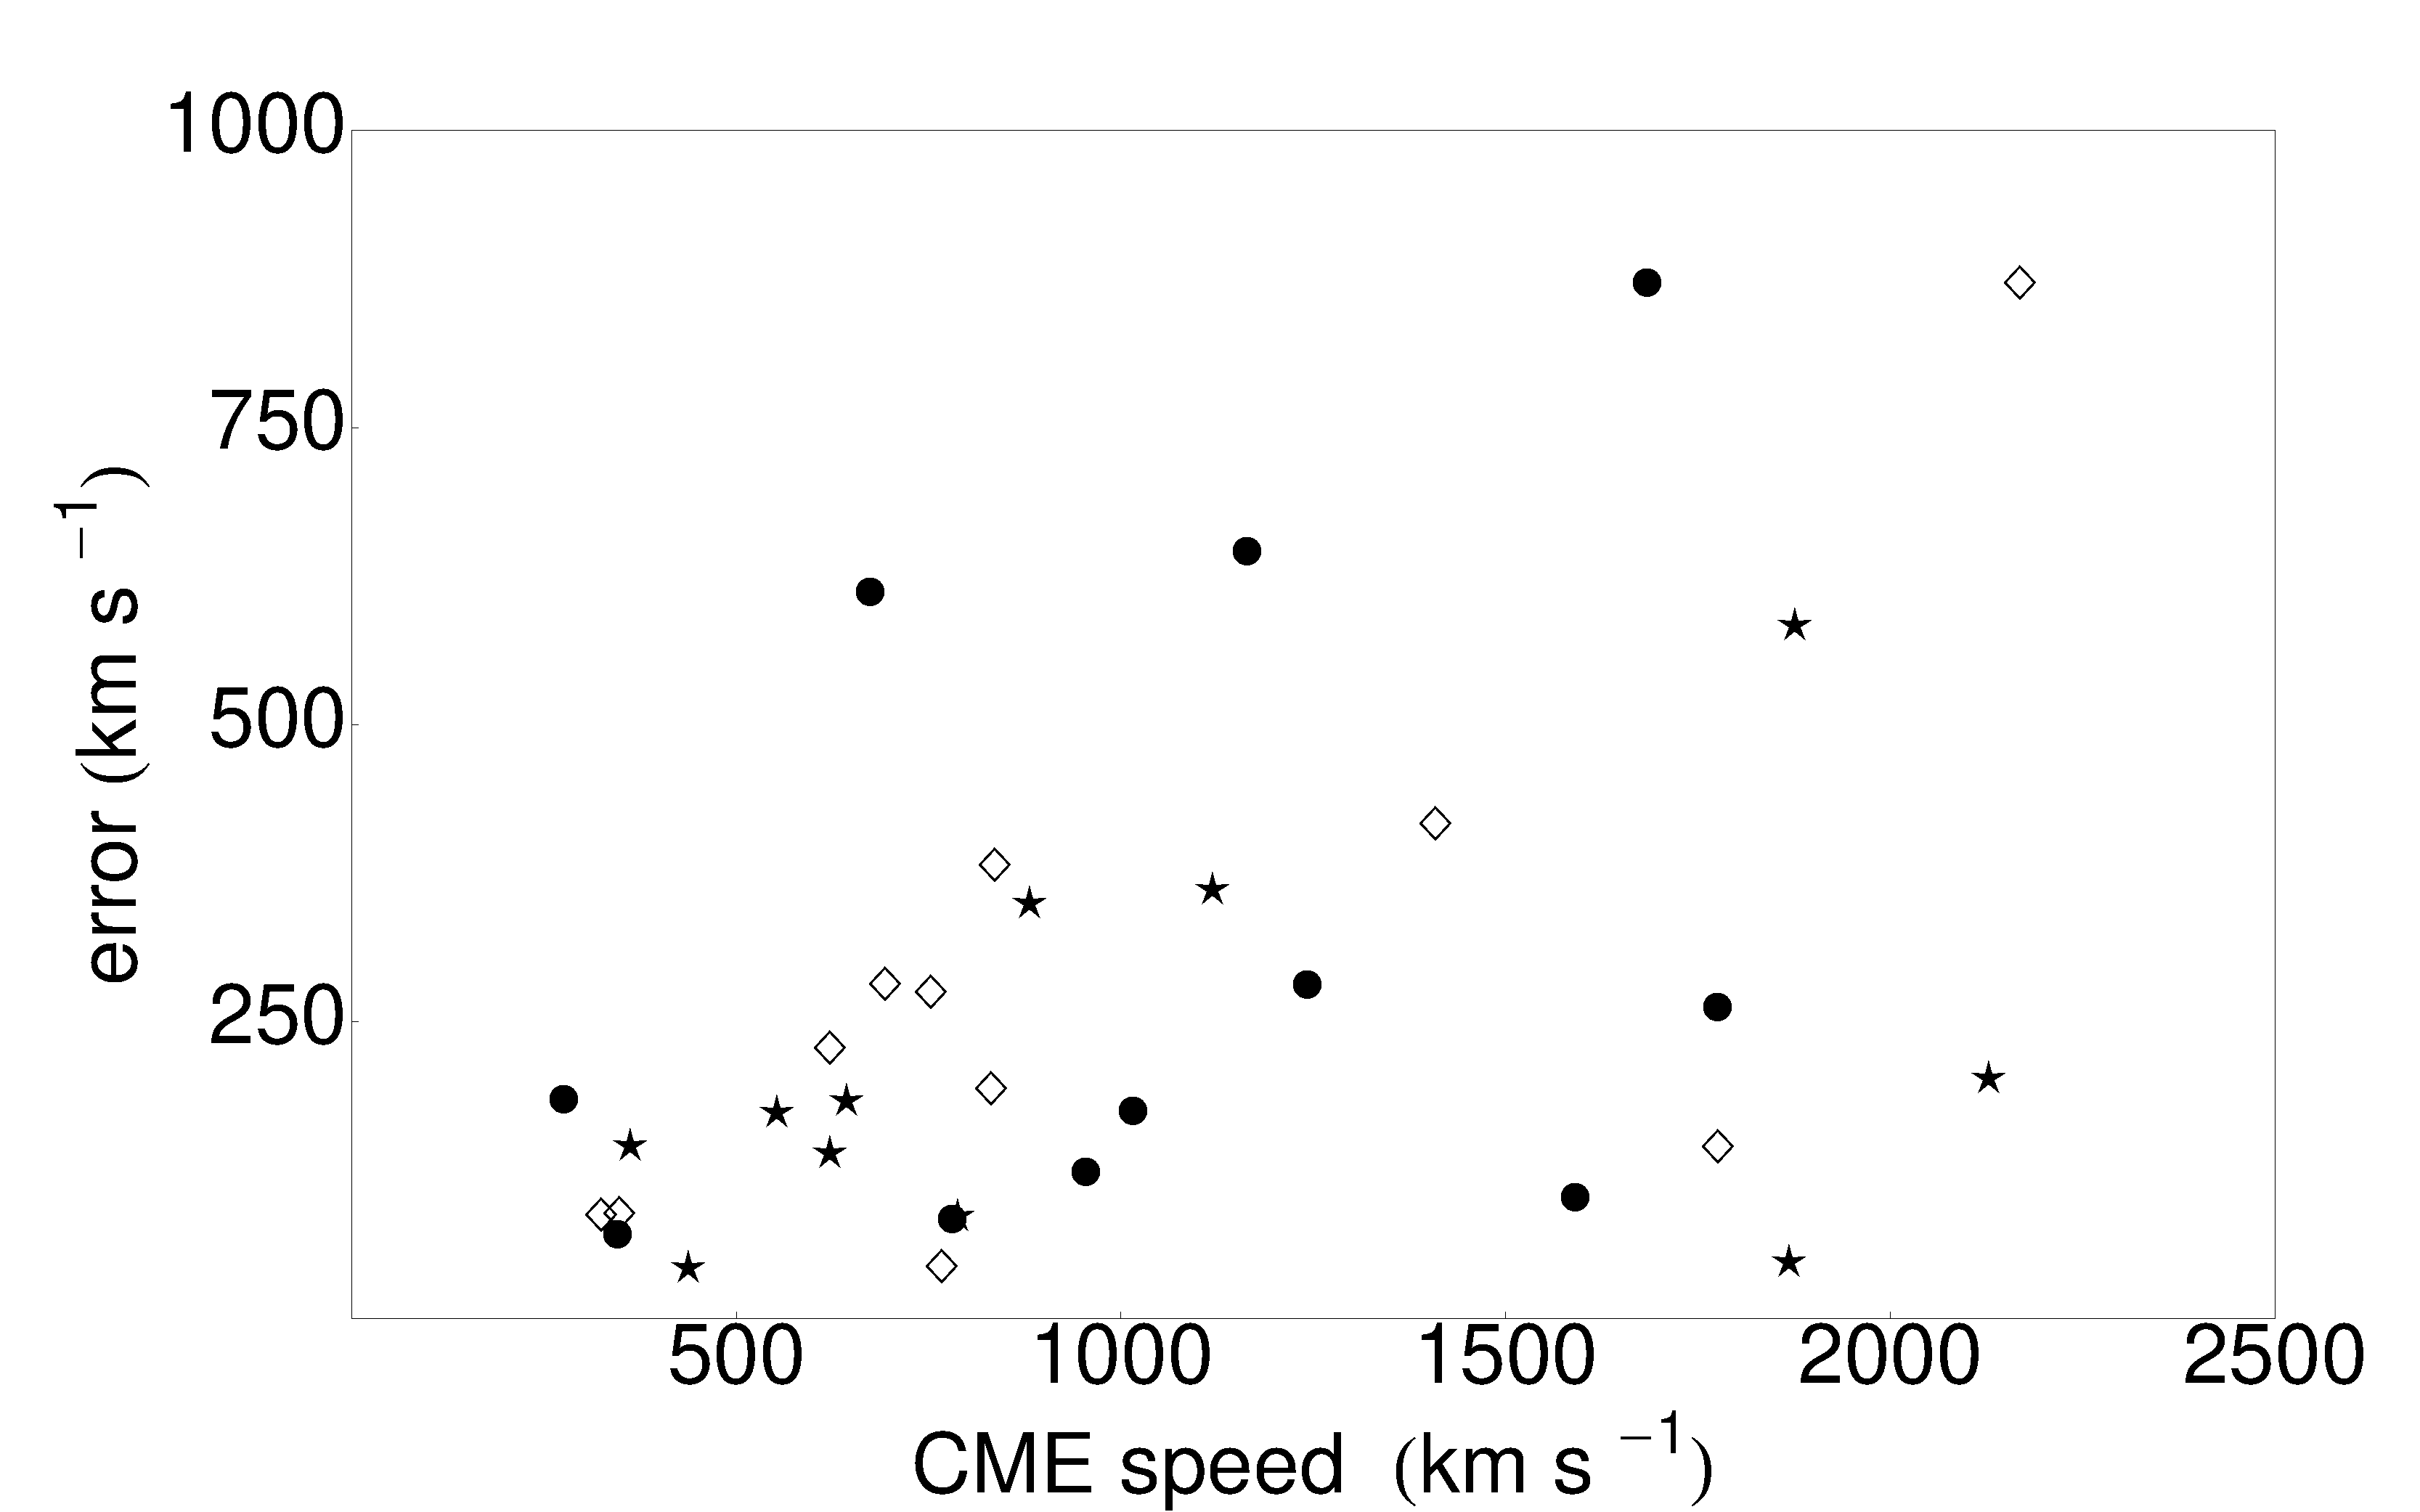
\includegraphics[width=0.48\hsize]{chapter2/figs/Fig_er_speed1.pdf}
	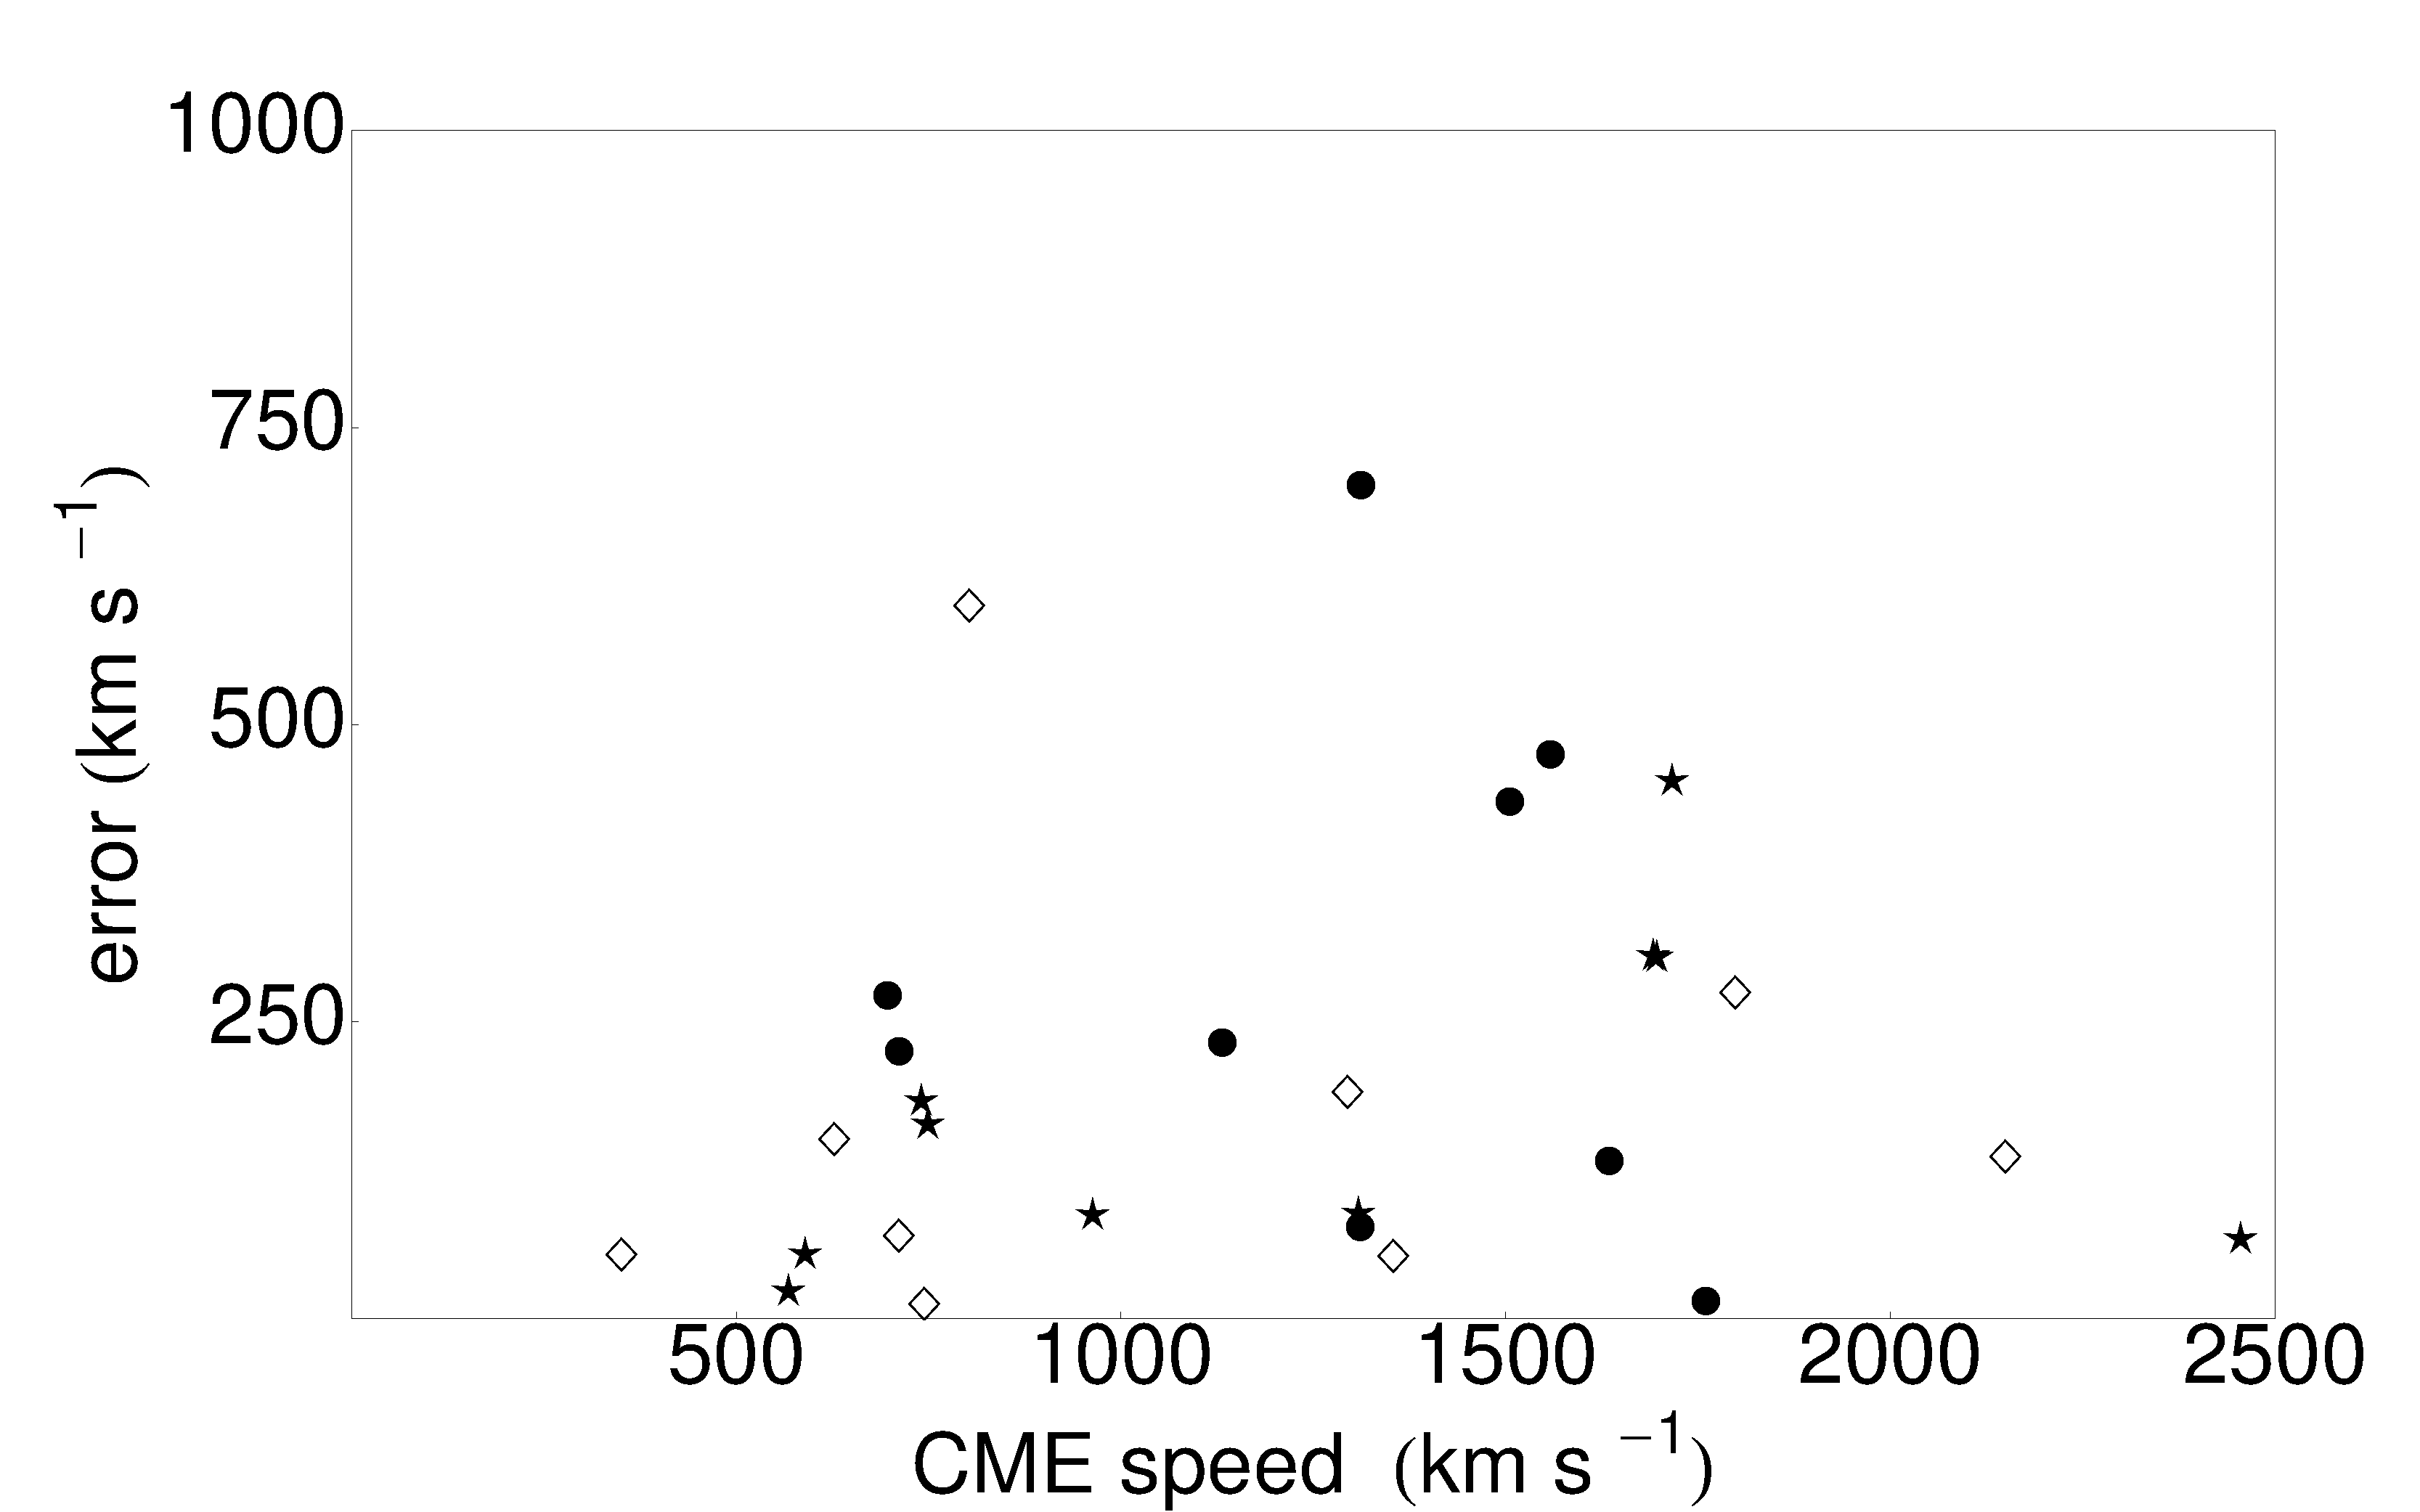
\includegraphics[width=0.48\hsize]{chapter2/figs/Fig_er_speed2.pdf}
	\caption{Scatter plot illustrates the comparison of 3D de-projected CME speeds derived from the spheroid model (depicted as diamonds), the ellipsoid model (represented by stars), and the GCS model (indicated as dots) versus the measurement errors for observers 1 (left) and 2 (right). Credit goes to \citet{miteva_2023}.}
	\label{fig_vcme_err}
\end{figure}

\subsubsection{Correlation between GSs, Coronal, and Near-Sun Parameters}
Figure~\ref{fig_speeds_dst} shows a scatter plot illustrating the relationship between the modulus of the GS Dst index and CME speed. Averaged results of three model fits (\textit{3D-mean}) are compared with 2D SOHO-LASCO CME speeds in Table~\ref{tab_cc_CME}, alongside error estimates from 3D de-projections. Despite some overlap, the largest error value among observers (as outlined in Table~\ref{tab_fits}) is highlighted for clarity.

Analysis reveals no discernible trend between the Dst index and CME speed, regardless of considering 3D de-projections or 2D CME speeds. Data constraints prevented 3D speed de-projections for the most robust GSs, skewing speed distribution and impacting findings. Despite the modest sample size (10 to 20 event pairs), Pearson correlations assess fit quality. Coefficients in Table~\ref{tab_cc_CME} range from negligible (e.g., 0.04 for 2D LASCO speeds) to moderate (highest: 0.55 with GCS model). Notably, no significant correlations are found between Dst index and other coronal parameters (e.g., SF class, location, CME AW), as comprehensively presented in the same table.

\begin{table}[!htp] 
	\small
	\centering
	\caption{Table displaying Pearson correlation coefficients among the GS Dst index, CME speed, and various solar parameters, with the respective sample sizes indicated in parentheses. Credit goes to \citet{miteva_2023}.}
	\label{tab_cc_CME}
	\begin{tabular}{llll}
		\toprule
		\textbf{CME source}	& \textbf{Dst$-$speed} & \textbf{solar parameter} & \textbf{Dst$-$solar parameter}	\\
		\midrule
		LASCO              & 0.04 (20) & SF class      & $-$0.04 (14) \\
		{\bf 3D - mean}    & {\bf 0.49 (12)} & SF latitude   & $-$0.16 (14)   \\
		3D spheroid - mean & 0.34 (12) & SF longitude  & 0.13 (14)	\\
		3D spheroid - obs1 & 0.14 (11) & CME AW        & 0.03 (20) \\
		3D spheroid - obs2 & 0.15 (10) & \\ 
		3D ellipsoid - mean & 0.53 (12) & &	\\
		3D ellipsoid - obs1 & 0.28 (11) & & \\
		3D ellipsoid - obs2 & 0.40 (10) & &\\
		3D GCS - mean & 0.55 (12) & &\\
		3D GCS - obs1 & 0.49 (11) & &\\
		3D GCS - obs2 & 0.27 (10) & & \\
		\bottomrule
	\end{tabular}
\end{table}

\begin{figure}[!htp]
	\centering
	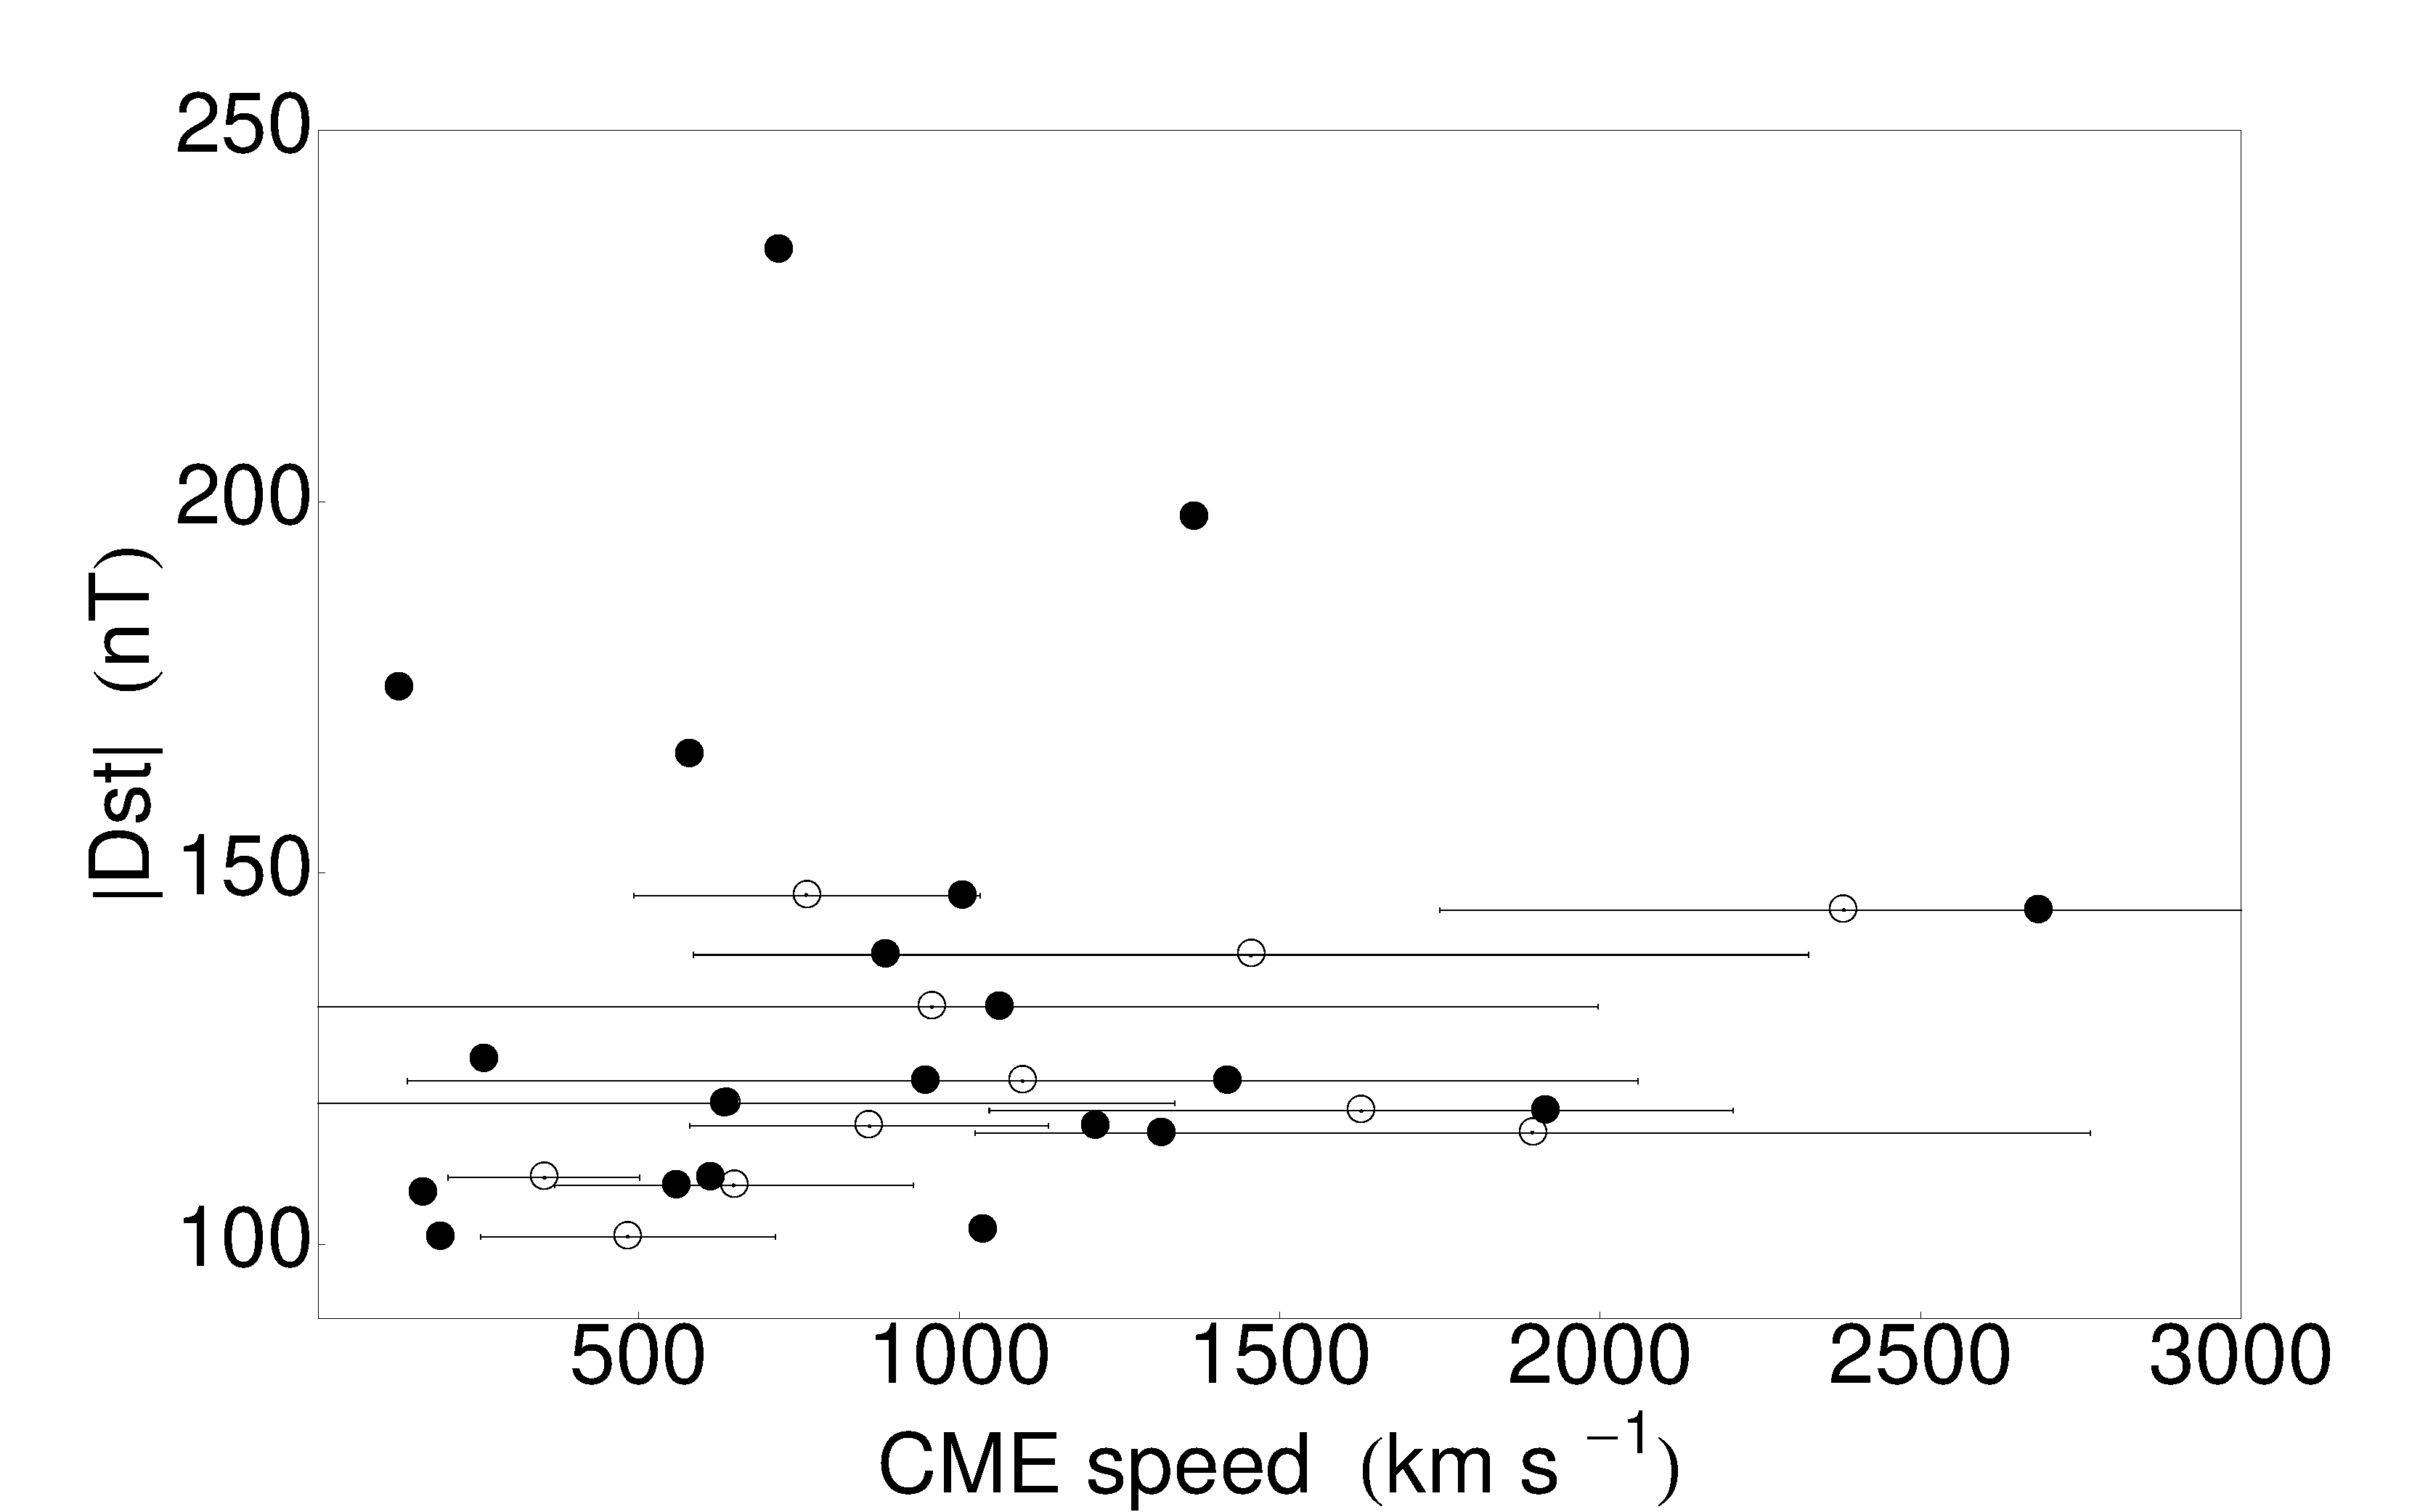
\includegraphics[width=0.7\hsize]{chapter2/figs/Fig_GS_speed_er_mean.pdf}
	\caption{Scatter plot illustrating the relationship between the Dst index and CME speed, incorporating data from the SOHO/LASCO instrument (represented by filled circles) and 3D de-projections (depicted by empty circles). Credit goes to \citet{miteva_2023}.}
	\label{fig_speeds_dst}
\end{figure}

\begin{figure}[!htp]
	\centering
	\begin{subfigure}[b]{0.45\textwidth}
		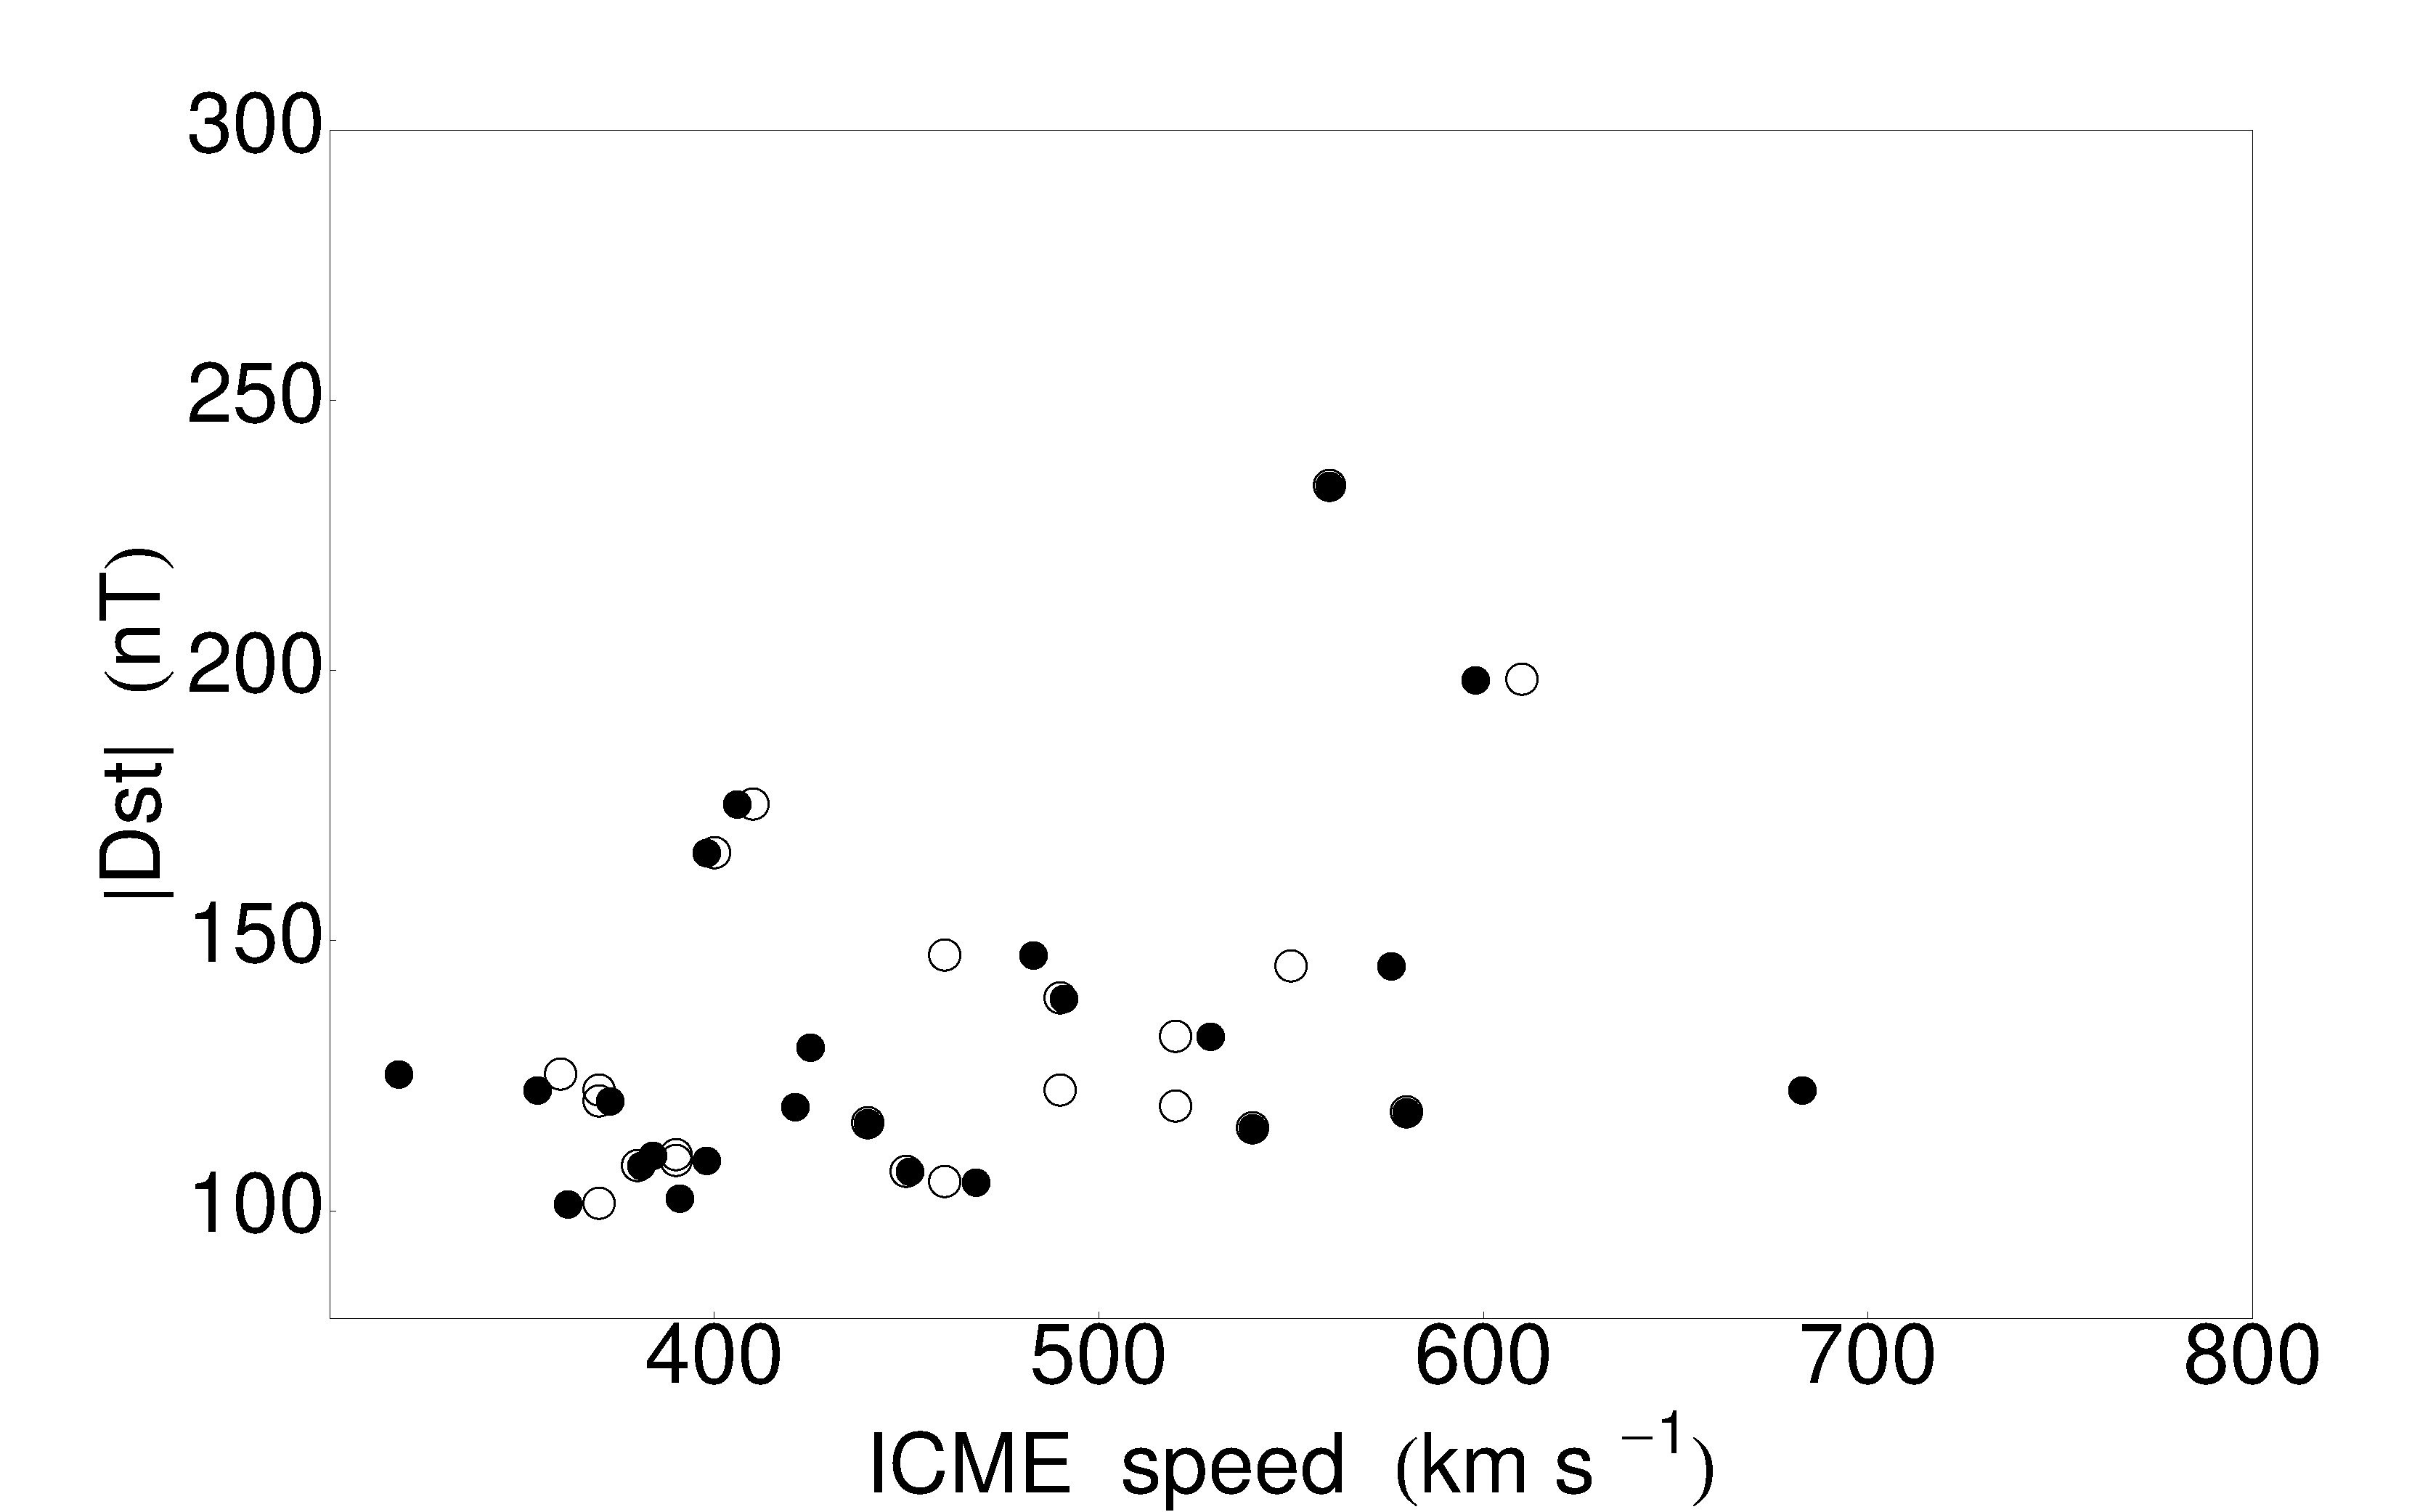
\includegraphics[width=\textwidth]{chapter2/figs/Fig_GS_ICMEspeed.pdf}
	\end{subfigure}
	\hfill
	\begin{subfigure}[b]{0.45\textwidth}
		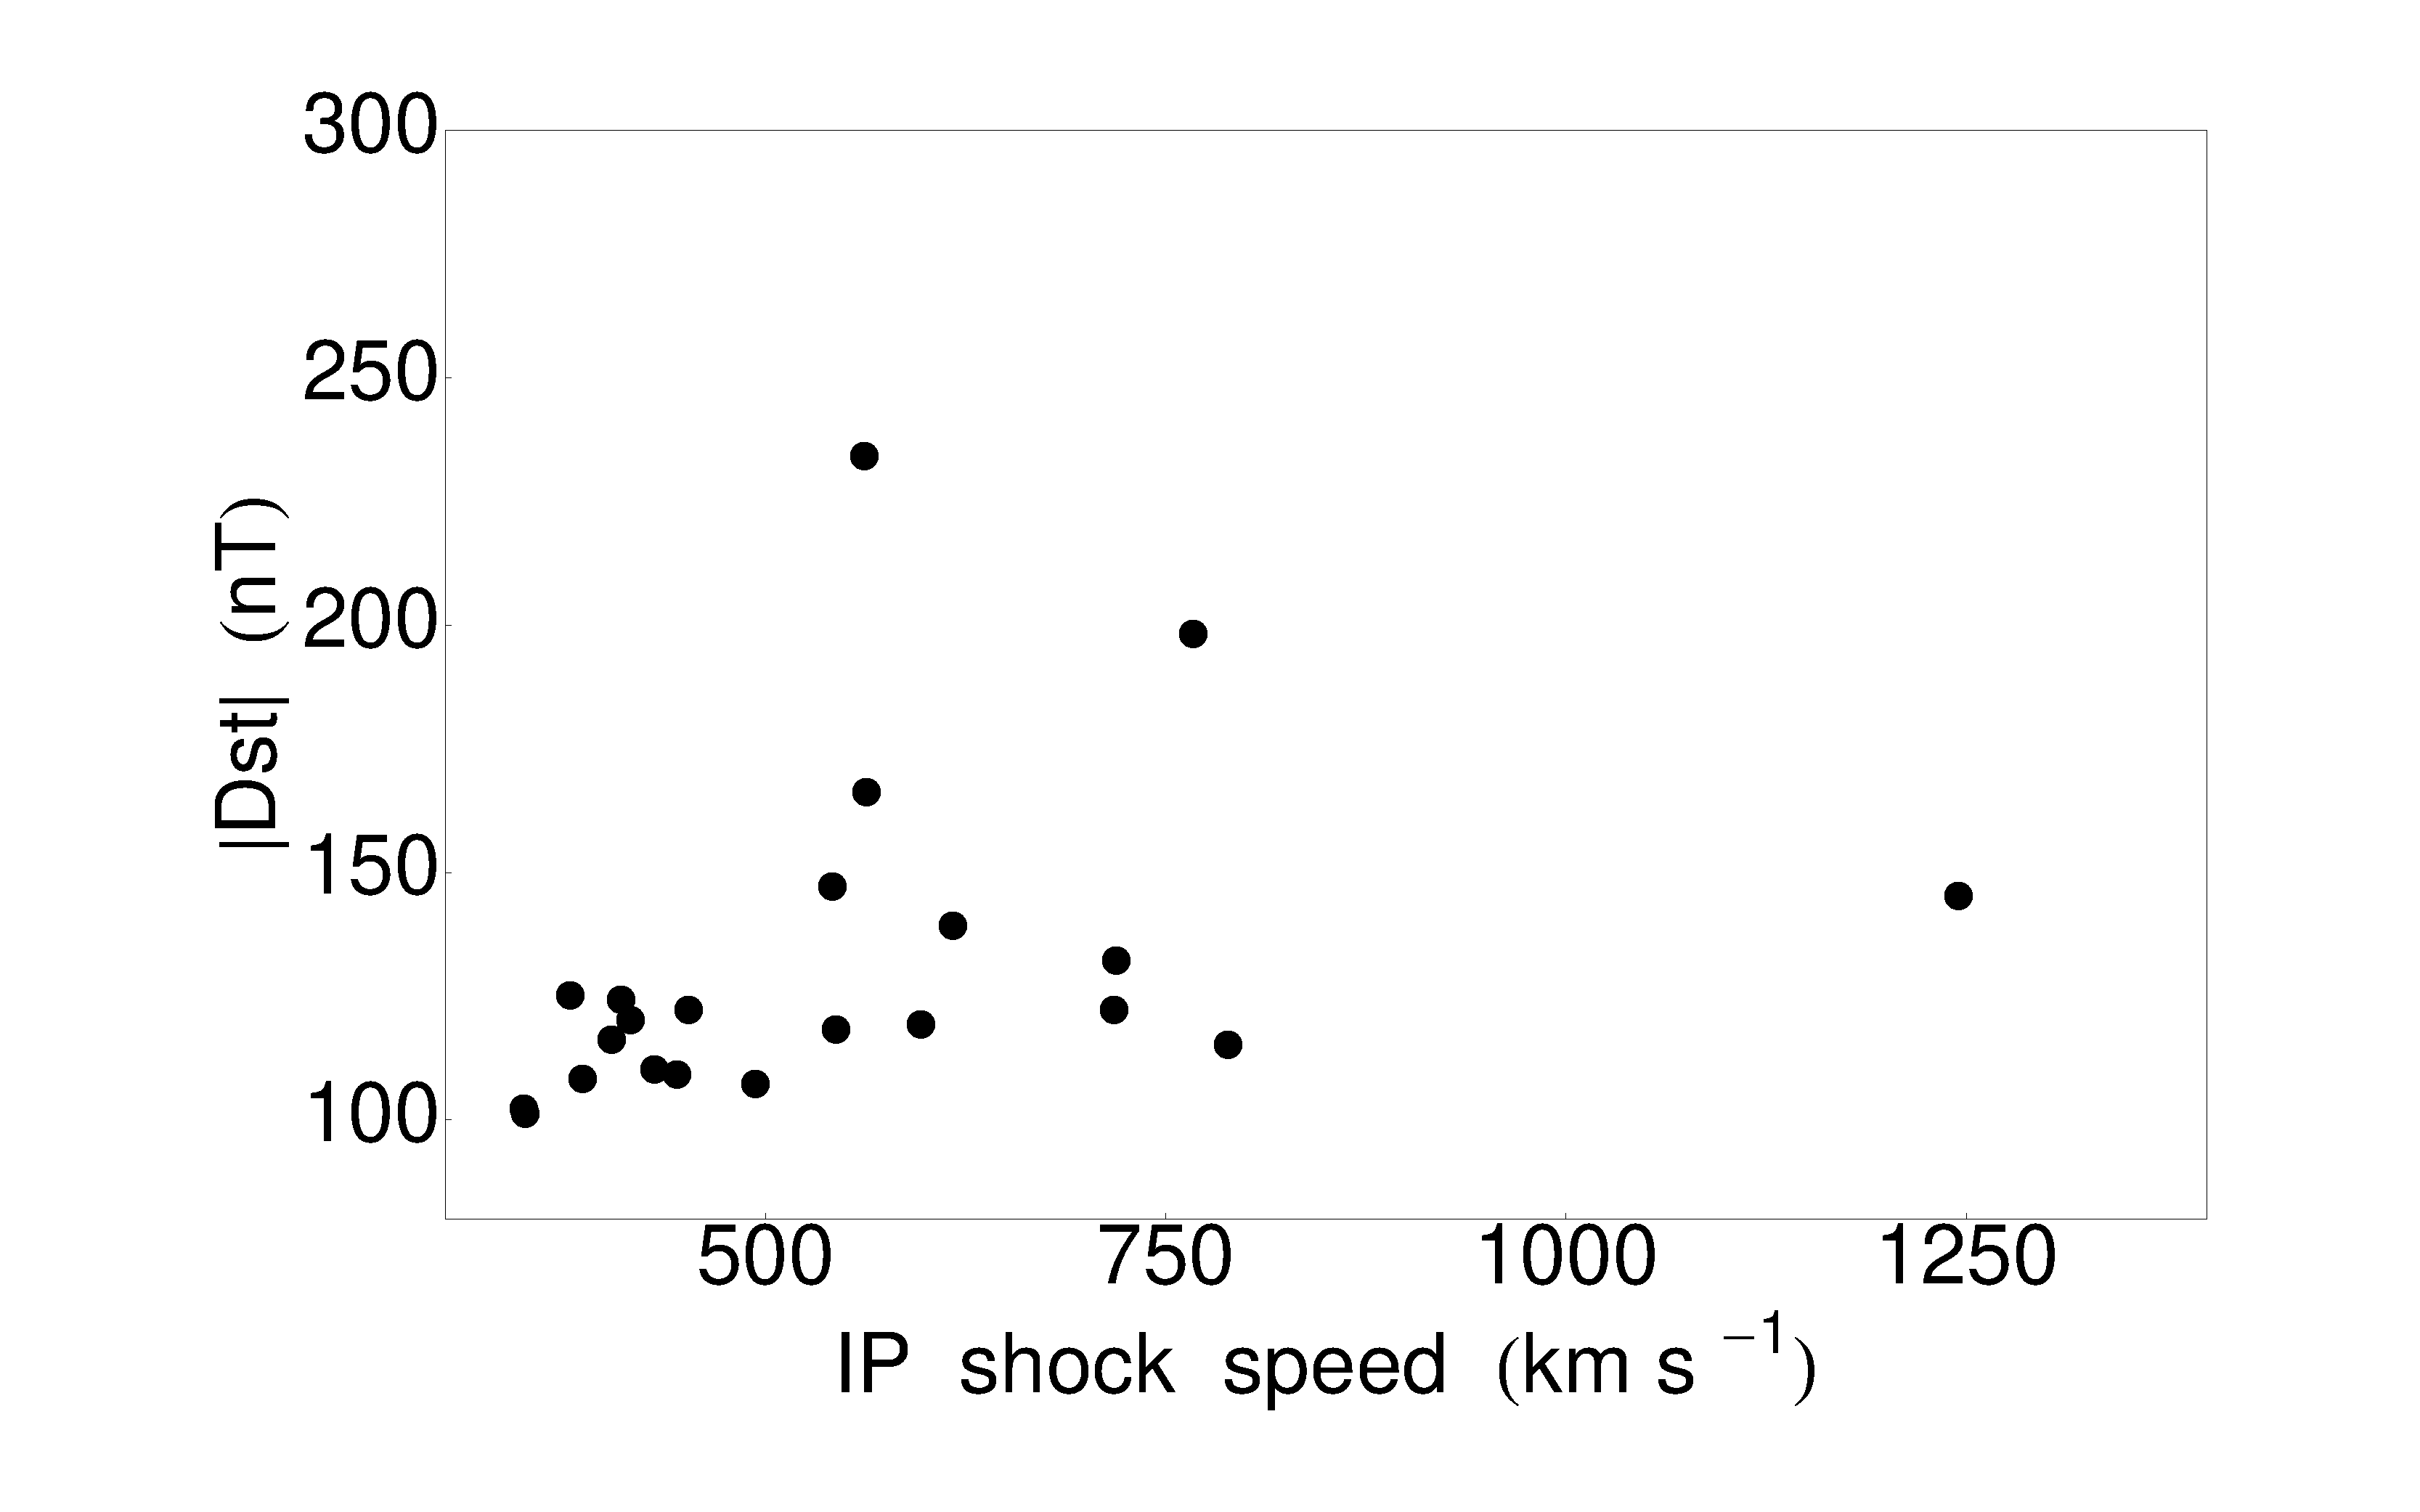
\includegraphics[width=\textwidth]{chapter2/figs/Fig_GS_IPspeed.pdf}
	\end{subfigure}
	\begin{subfigure}[b]{0.45\textwidth}
		\includegraphics[width=\textwidth]{chapter2/figs/Fig_GS_Ms.pdf}
	\end{subfigure}
	\hfill
	\begin{subfigure}[b]{0.45\textwidth}
		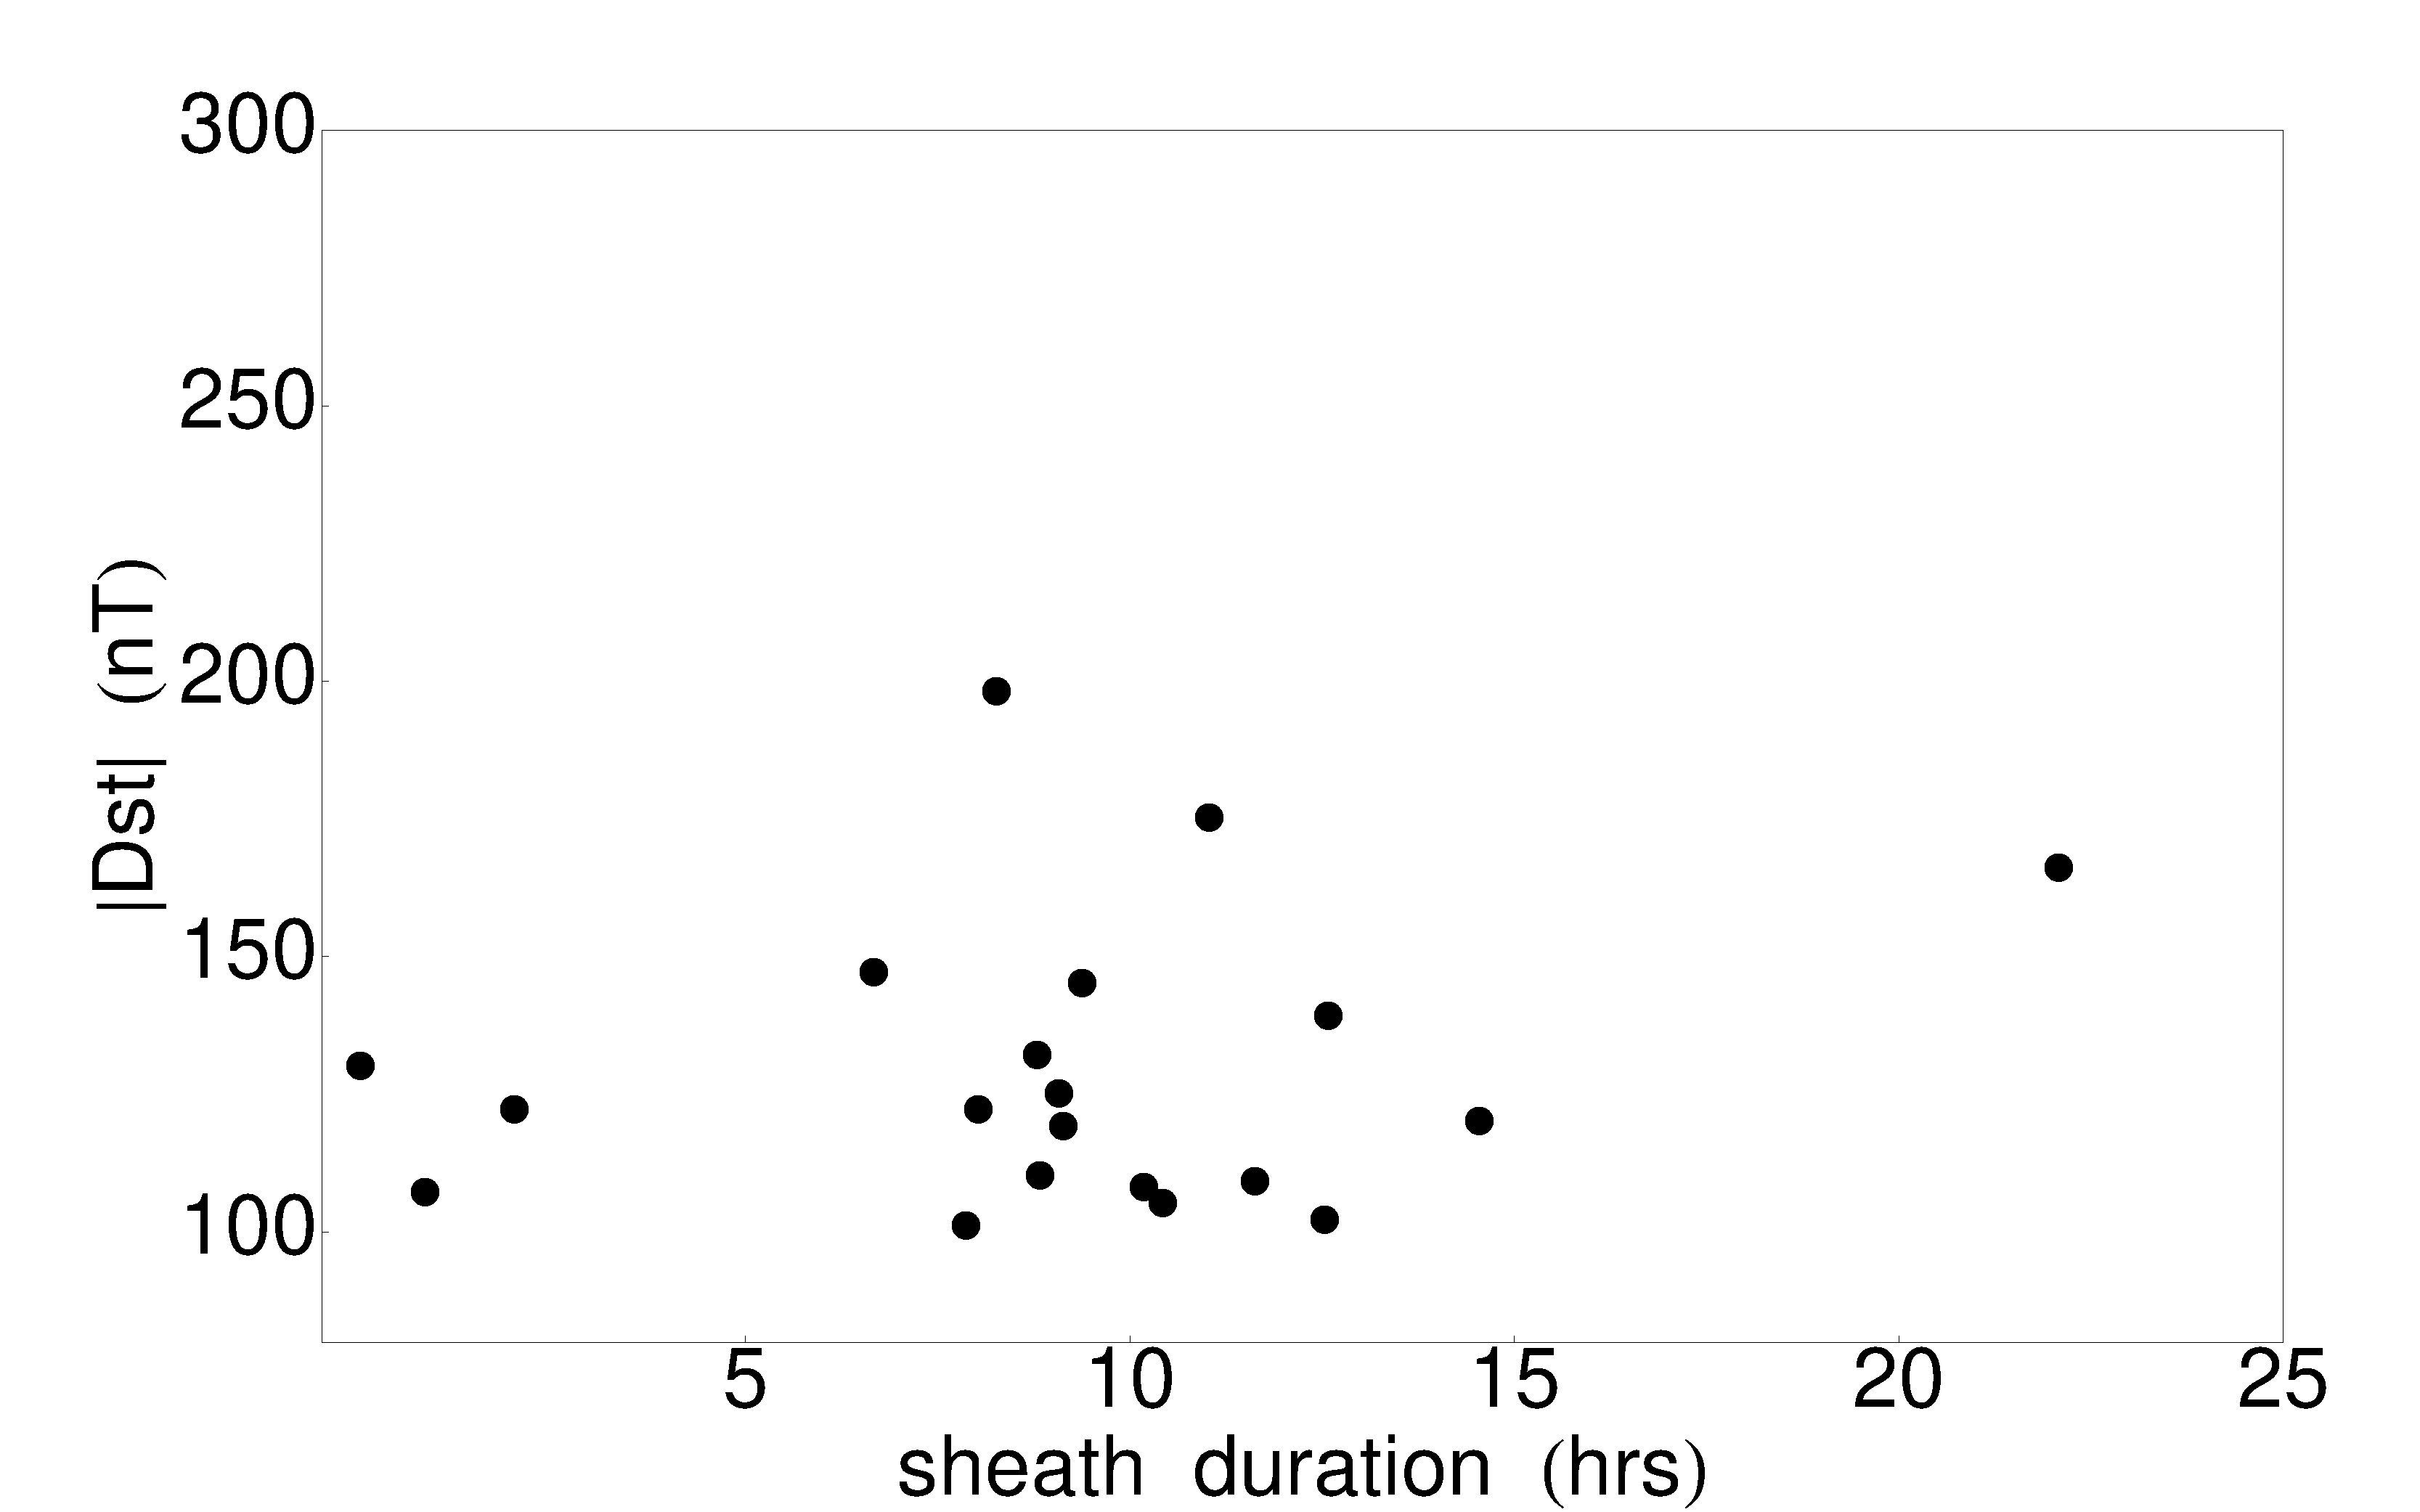
\includegraphics[width=\textwidth]{chapter2/figs/Fig_GS_sheath.pdf}
	\end{subfigure}
	\begin{subfigure}[b]{0.45\textwidth}
		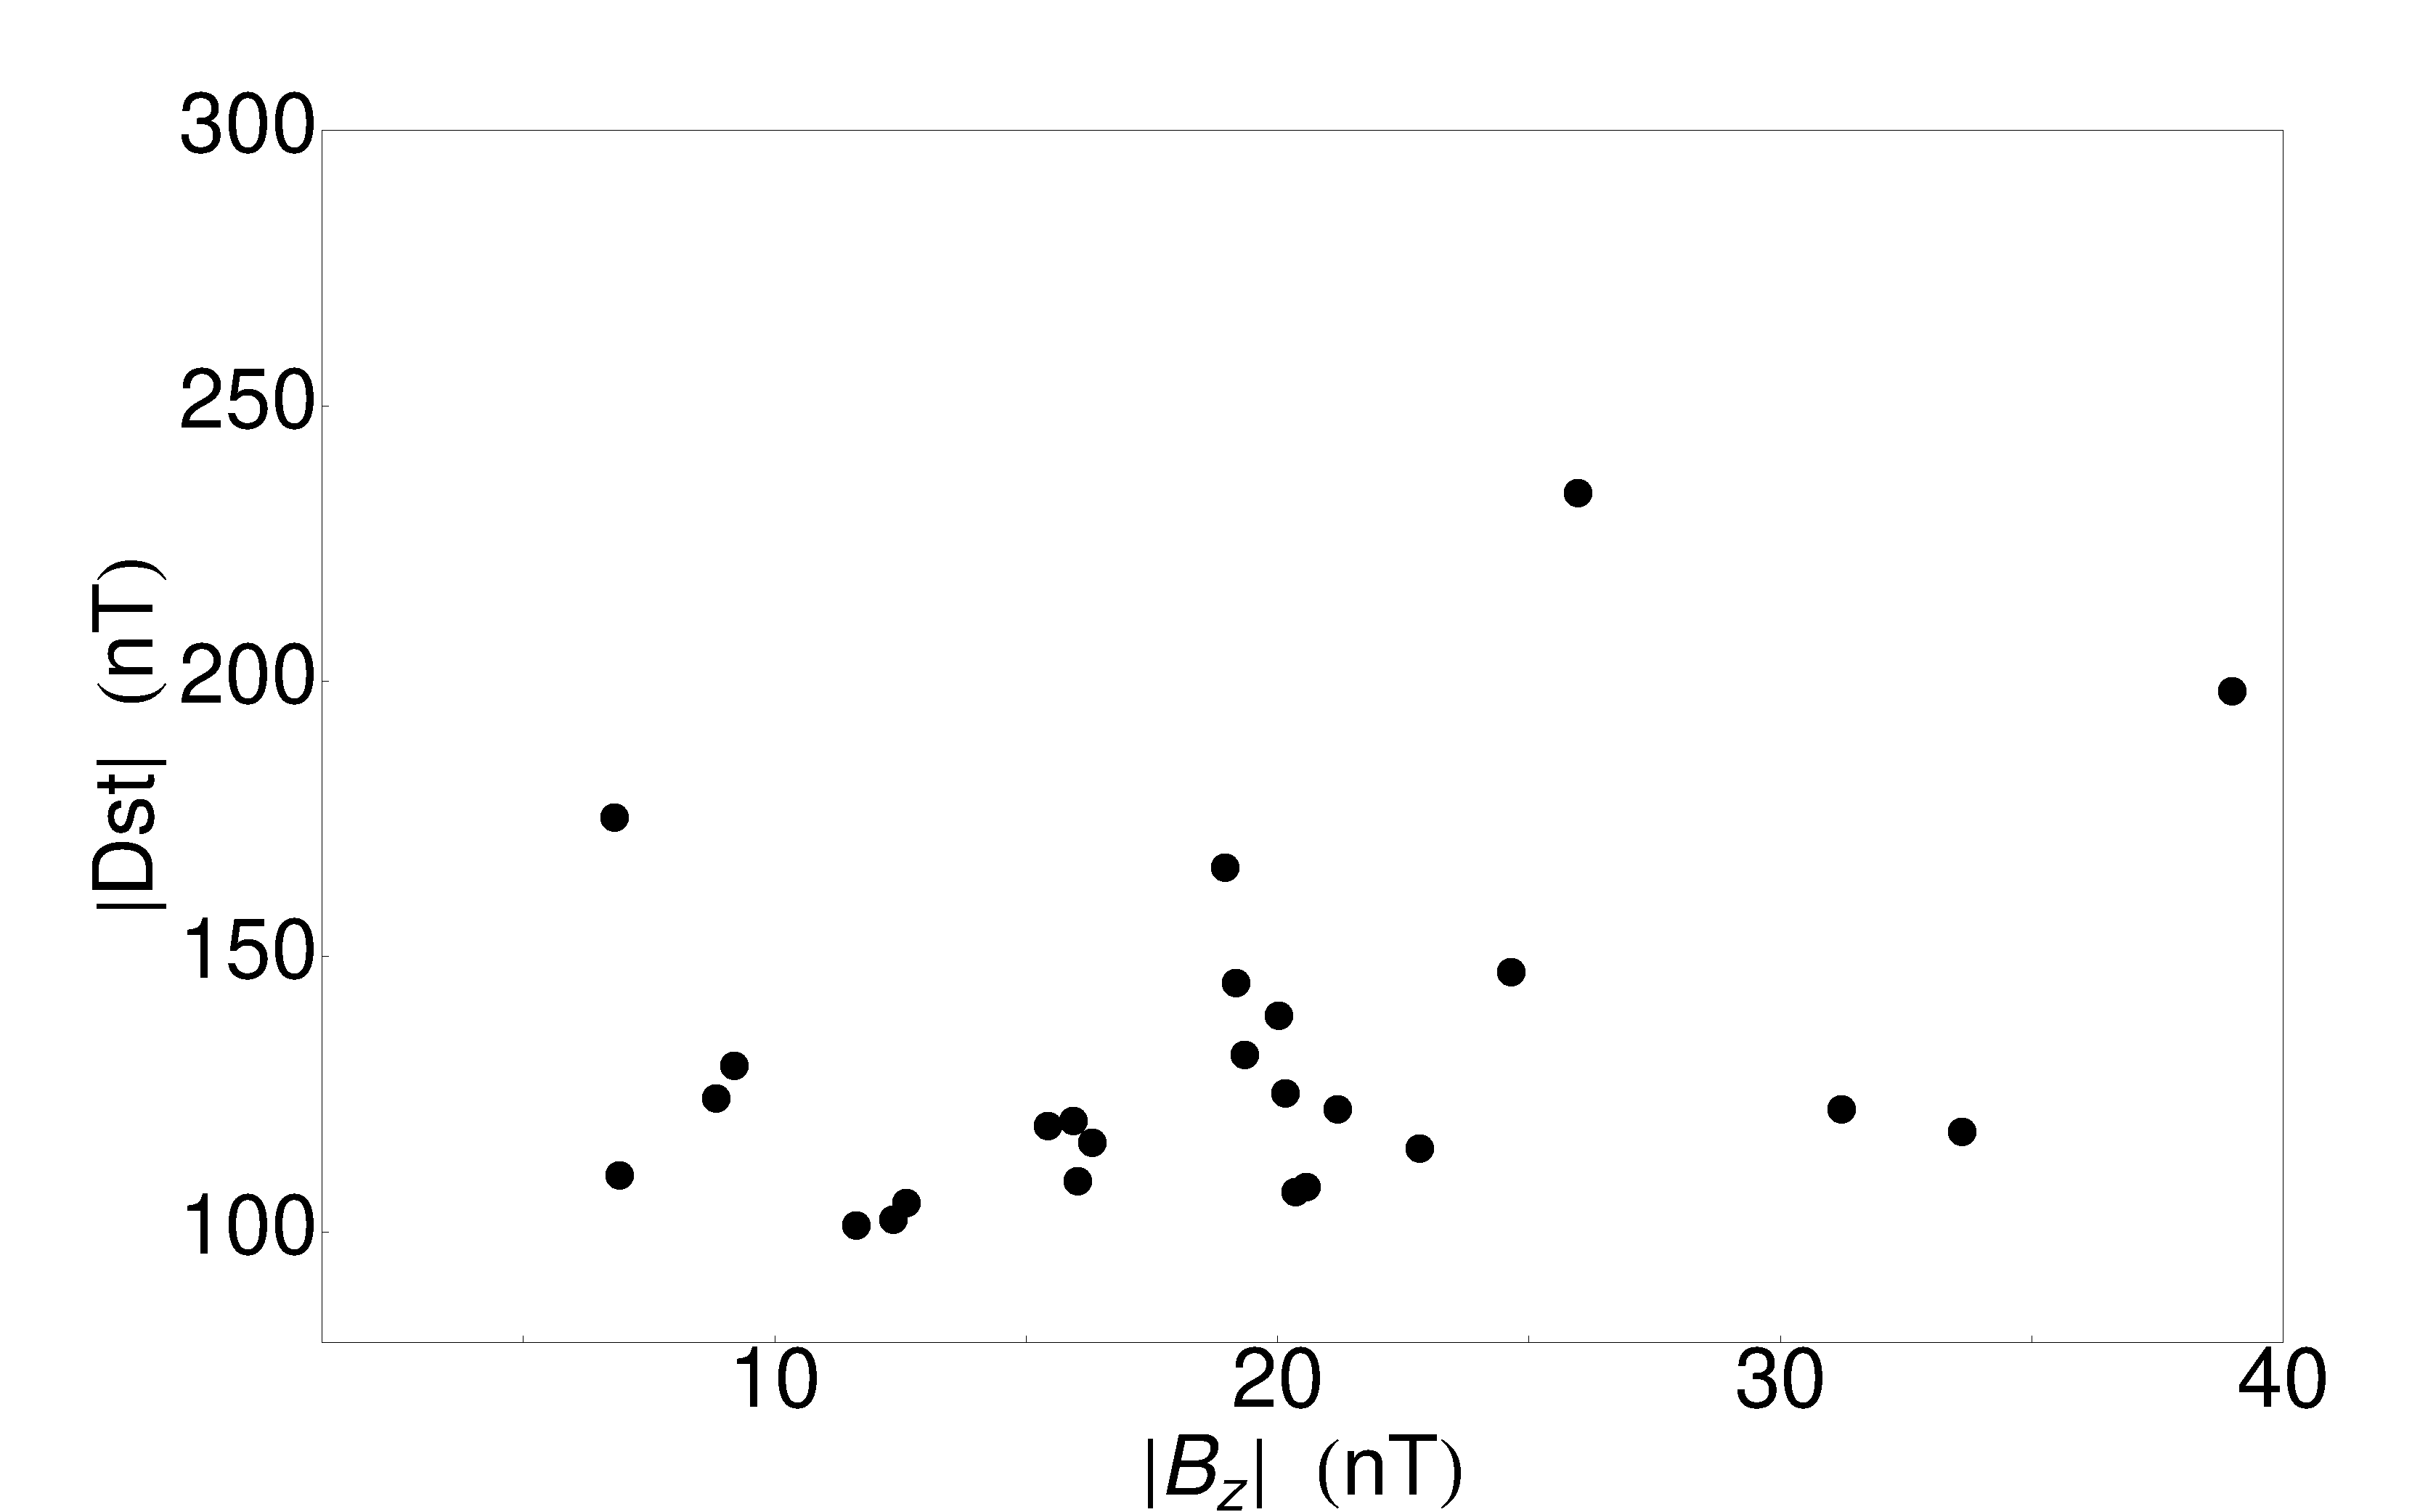
\includegraphics[width=\textwidth]{chapter2/figs/Fig_GS_Bz.pdf}
	\end{subfigure}
	\hfill
	\begin{subfigure}[b]{0.45\textwidth}
		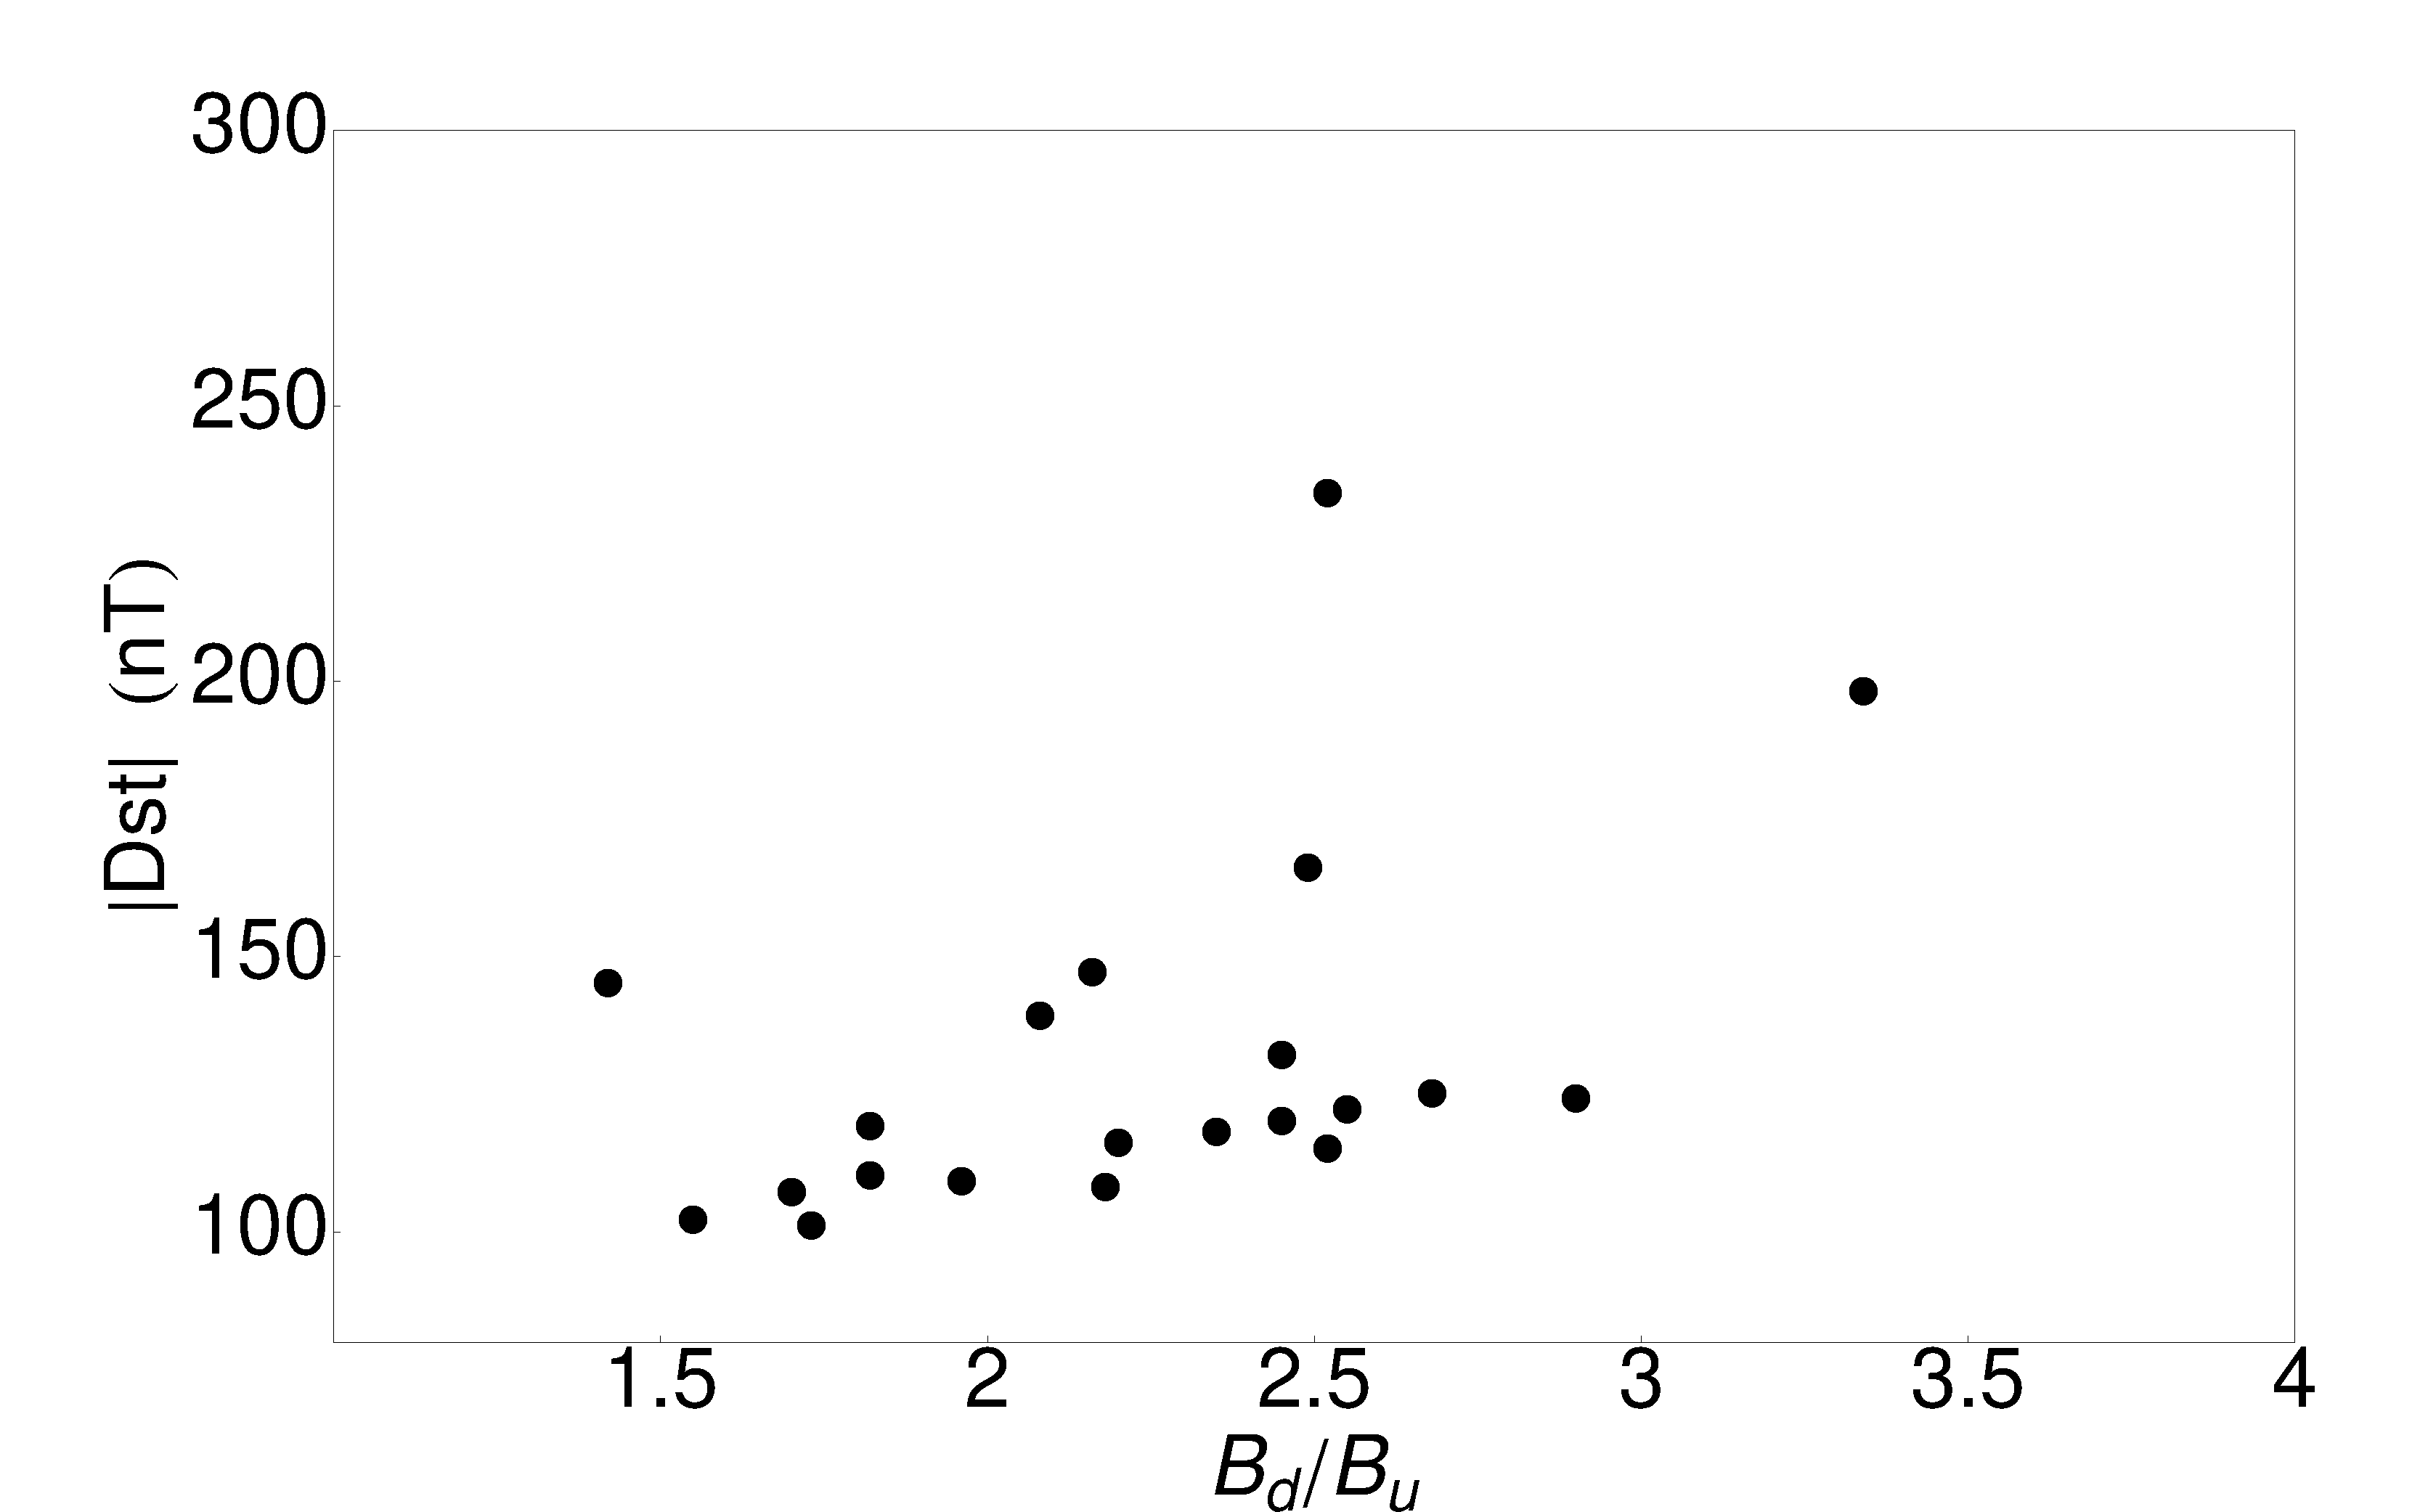
\includegraphics[width=\textwidth]{chapter2/figs/Fig_GS_Bjump.pdf}
	\end{subfigure}
	\begin{subfigure}[b]{0.45\textwidth}
	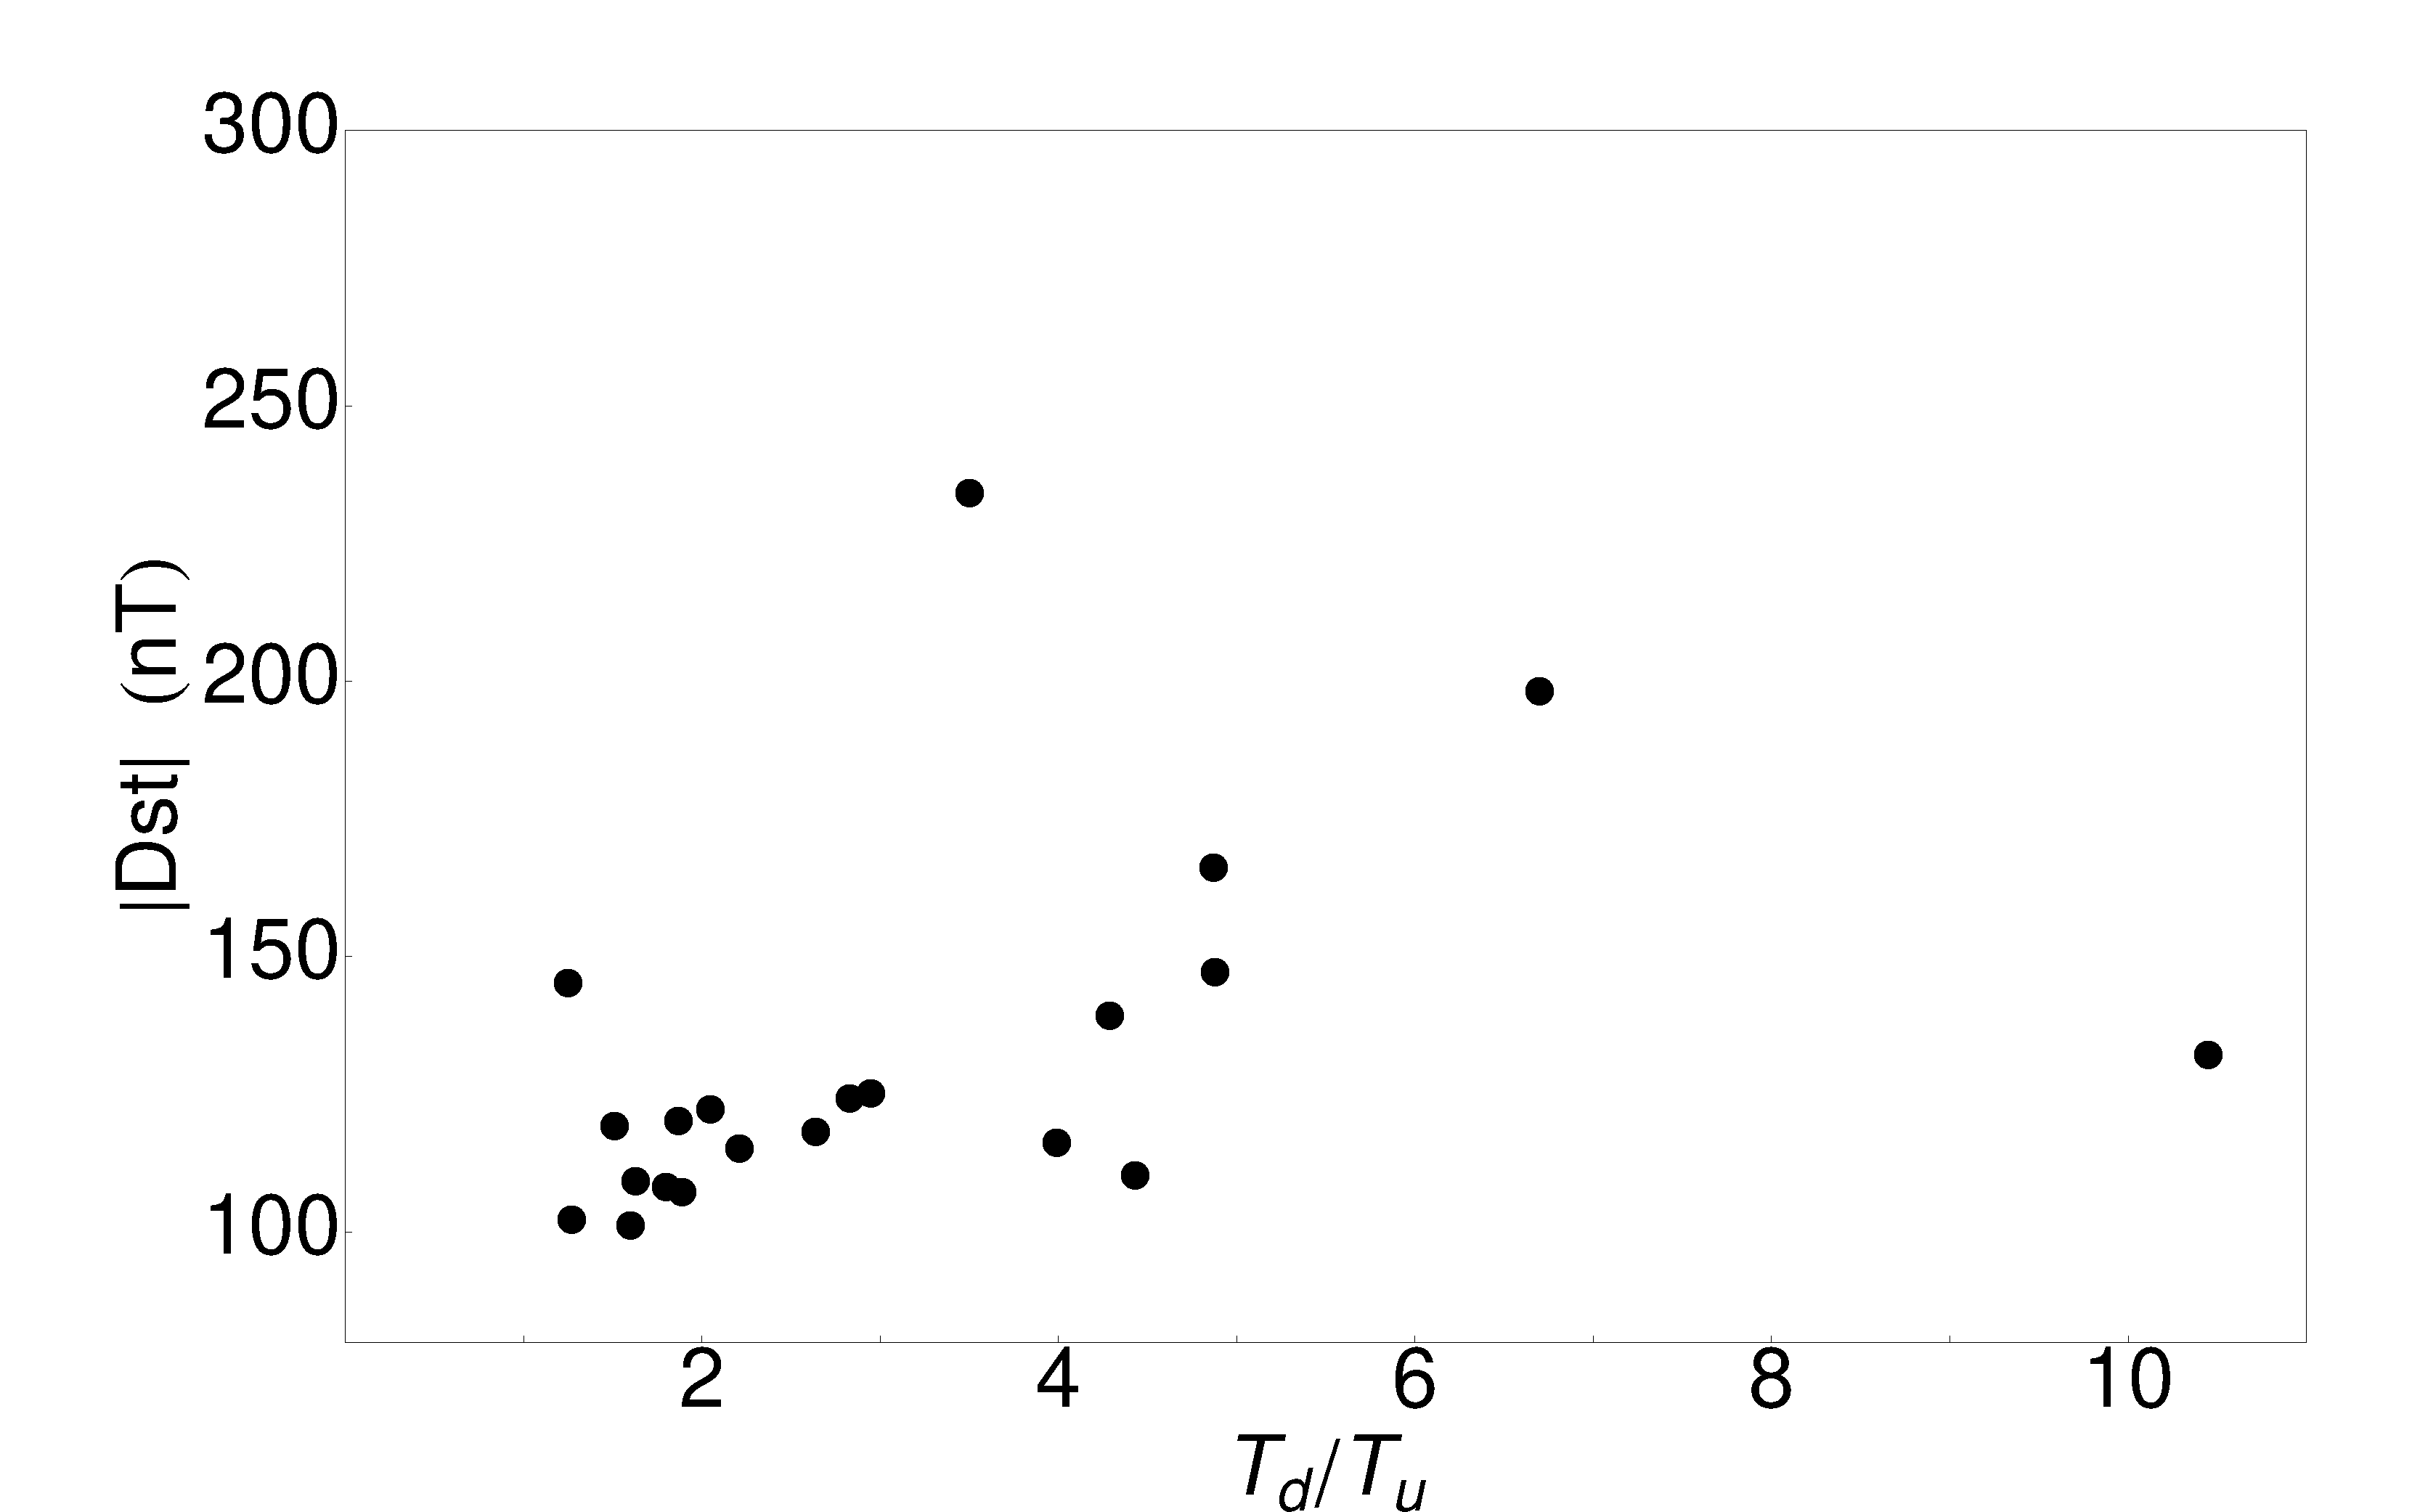
\includegraphics[width=\textwidth]{chapter2/figs/Fig_GS_Tjump.pdf}
\end{subfigure}
	\hfill
\begin{subfigure}[b]{0.45\textwidth}
	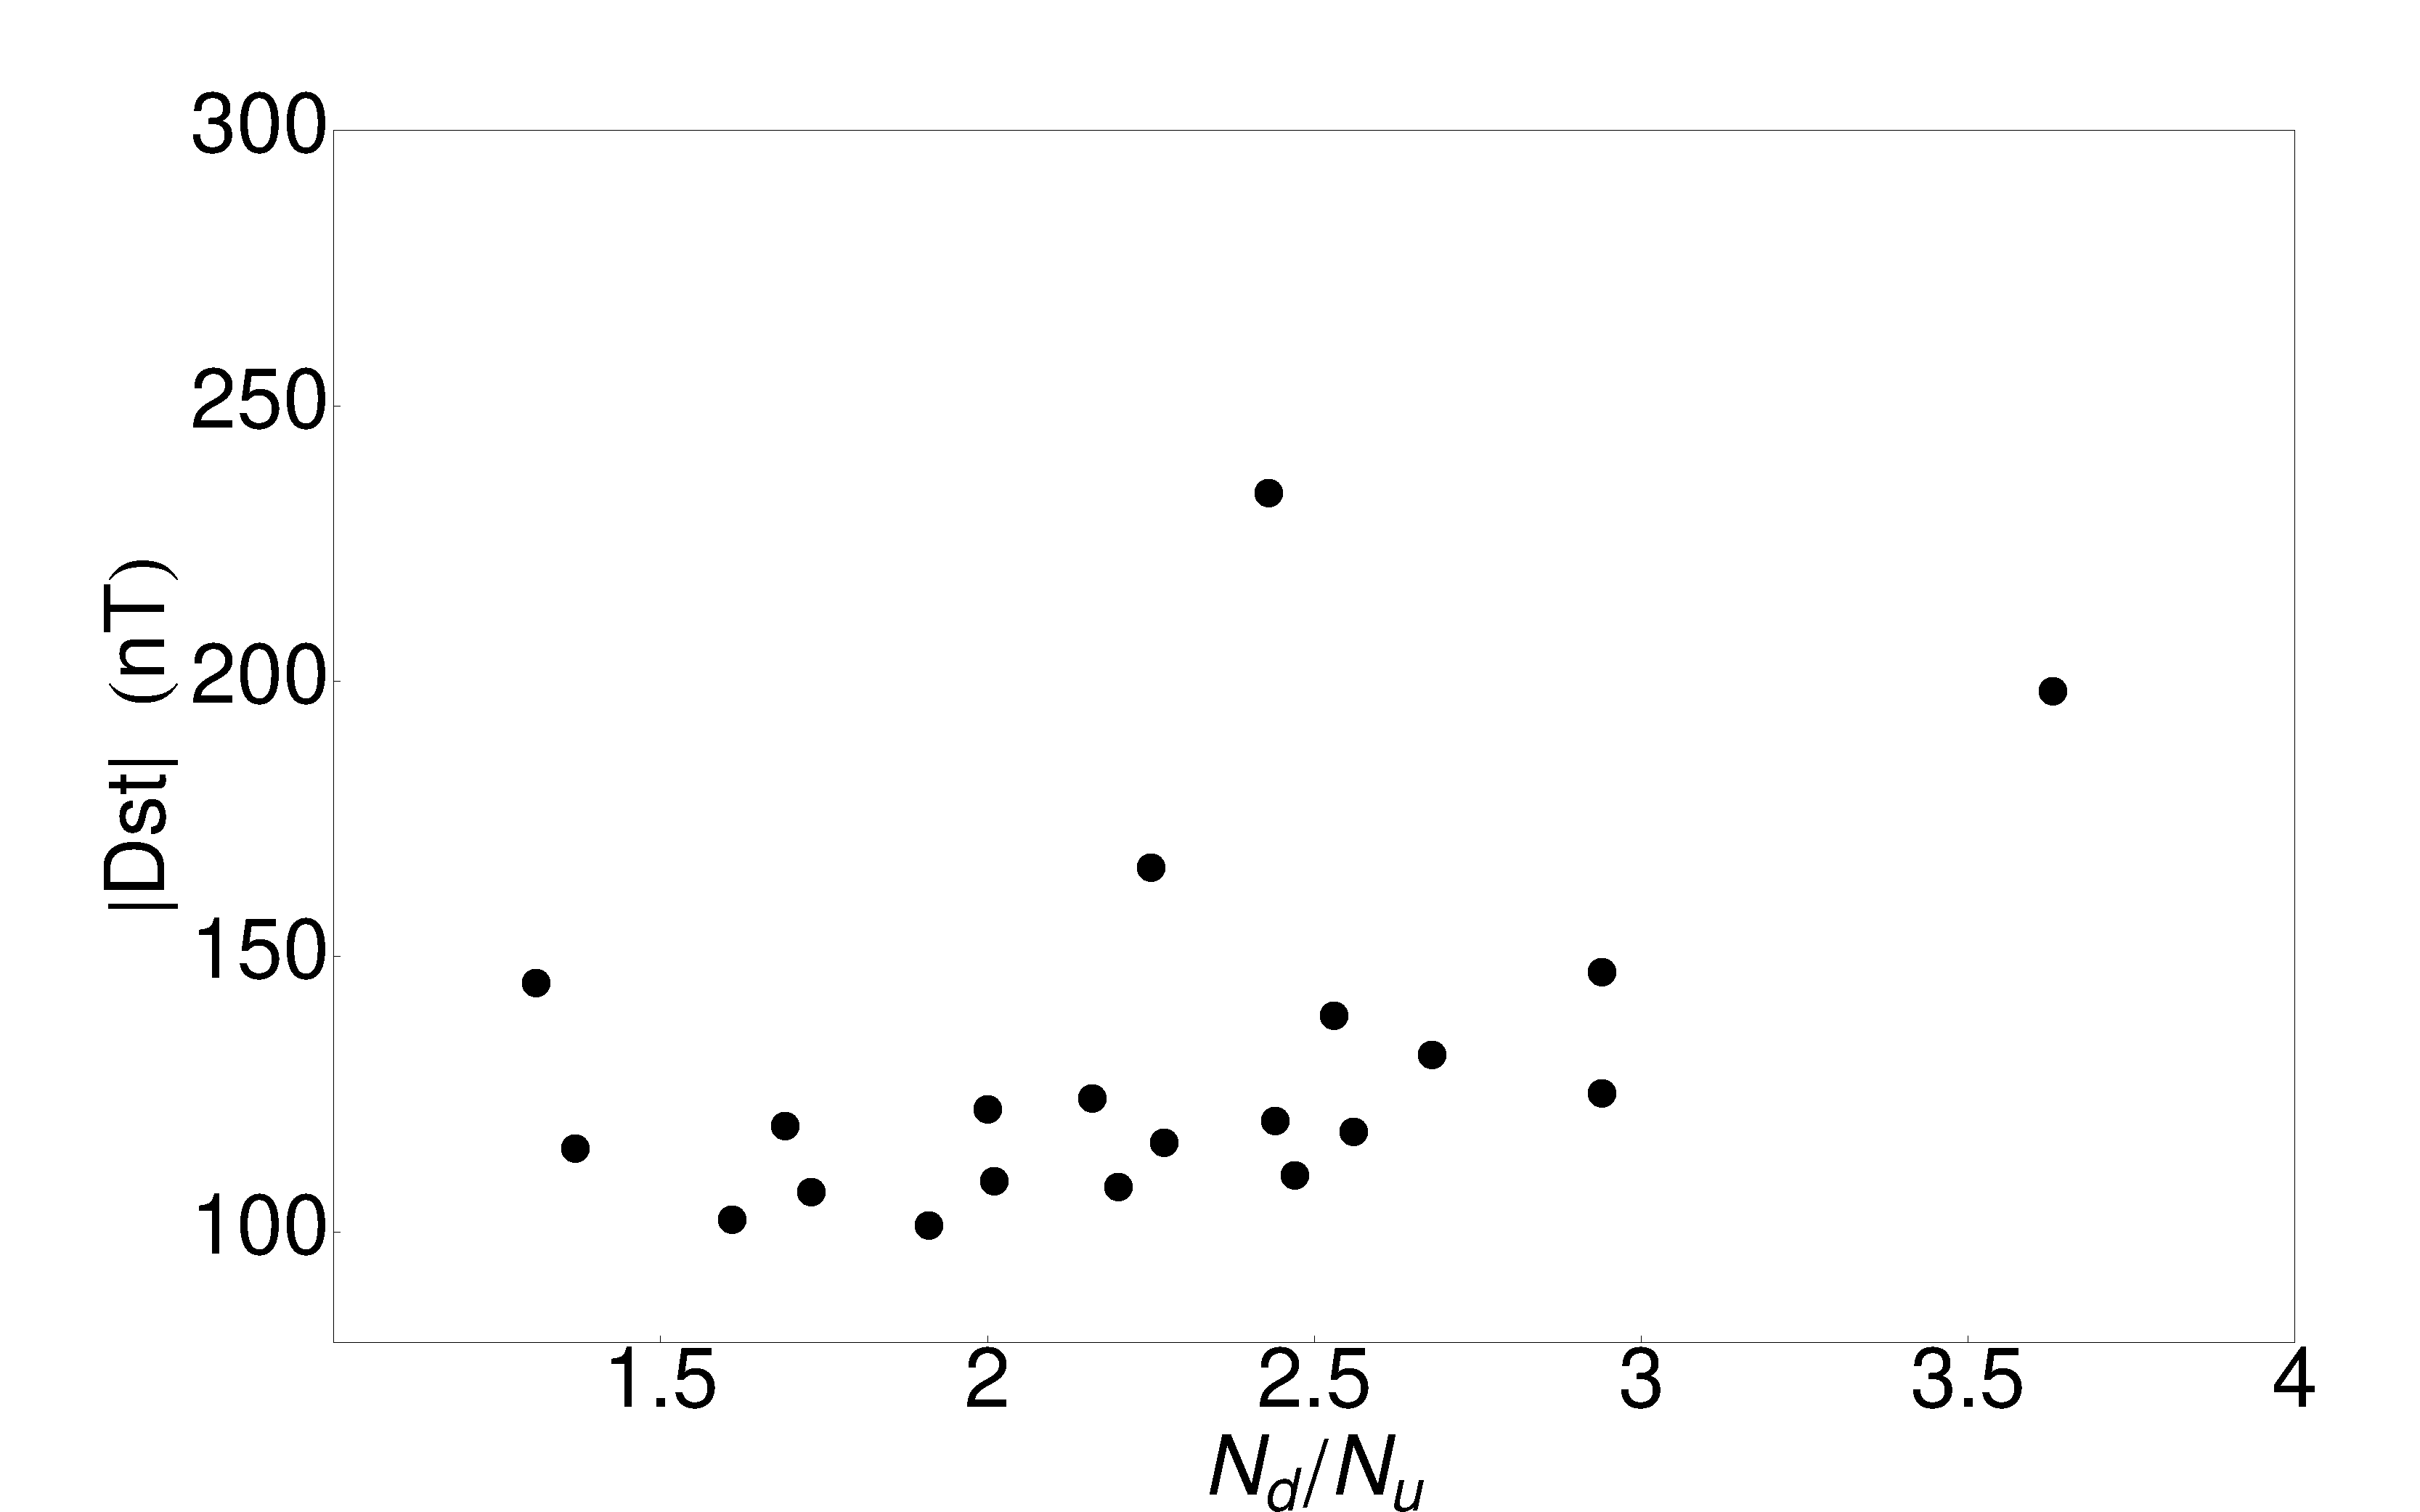
\includegraphics[width=\textwidth]{chapter2/figs/Fig_GS_Njump.pdf}
\end{subfigure}
	\caption{Comprehensive scatter plots illustrating the relationships between Dst index and various solar wind parameters, including Wind/ACE ICME speed, IP shock speed, Mach number, duration of sheath region, Bz, magnetic field jump, temperature jump, and density jump. Credit goes to \citet{miteva_2023}.}
	\label{fig_dst_scatterplots}
\end{figure}

\begin{table}[!htp] 
	\small
	\centering
	\caption{Tabular representation of Pearson correlation coefficients between the GS Dst index and various parameters of IP phenomena. The data is derived from Wind satellite measurements, unless otherwise stated, with the corresponding sample sizes indicated in parentheses. Credit goes to \citet{miteva_2023}.}
	\label{tab_cc_IP}
	\begin{tabular}{lc}
		\toprule
		\textbf{IP parameter} & \textbf{Dst$-$IP parameter} \\
		\midrule
		ICME speed  & 0.37 (24)	\\
		ICME speed (ACE)   & 0.44 (22)	\\
		IP shock speed  & 0.35 (22)	\\
		Mach number  & 0.36 (21)	\\ 
		sheath duration & 0.22 (20) \\
		$|B_z|$      & 0.37 (25) \\
		$B_d/B_u$  & 0.48 (21)	\\
		$T_d/T_u$  & 0.40 (21)	\\
		$N_d/N_u$  & 0.46 (21)	\\
		{\bf $B$}  & {\bf $-$0.14 (20)}  \\
		{\bf $V$}       & {\bf 0.19 (20)}	\\
		{\bf $\beta_u$} & {\bf $-$0.14 (21)}	\\
		\bottomrule
	\end{tabular}
\end{table}

\subsubsection{Correlation between GSs and IP Parameters}
We explore correlations between GSs and various parameters linked to pre-selected IP phenomena. Scatter plots illustrate relationships such as Dst index versus ICME speed and IP shock speed, Dst versus Mach number and sheath duration, and Dst versus $|Bz|$ and $B_d/B_u$. Figure~\ref{fig_dst_scatterplots} and Table~\ref{tab_cc_IP} detail these correlations.

For the limited sample used, we observe moderately positive trends between Dst index and plasma compression parameters at the shock interface, comparable to or slightly larger than correlations with ICME speeds. However, the trend with $|Bz|$ is weaker (0.37), contrasting with robust trends from prior studies. Correlations involving Dst and IP shock speed, Mach number, or sheath duration are relatively smaller.

Recent reports suggest strong correlations with electric and magnetic field components \citep{echer_2022}, although this exceeds our current analysis scope. Caution is warranted in interpreting results due to lack of uncertainty estimates for correlation coefficients. Additional parameters from ICME and IP shock catalogs show no robust correlations with Dst index, all correlation coefficients being smaller than 0.2.

\subsubsection{Forecasting GS Strength Based on Solar and IP Parameters}
We examine how magnetic obstacle type, orientation upon Earth arrival, and 3D reconstructed CME speeds collectively impact GS intensity, approximated by the Dst index.

The most potent GSs in our compilation exhibit distinctive magnetic structure parameters, including complexity, orientation, and speed at Earth. Exceptions include instances of fast speed flank hits or uncertain configurations, possibly influenced by fast solar wind streams or CIRs. Notably, IP structure associated with certain GSs has notably low speeds.

Interpretation considers information from both speed reconstructions and in situ measurements to enhance analysis robustness.

\section{Discussion}
The May 11, 2011 eruption showcased a variety of solar phenomena, including a fast partial-halo CME, a weak solar flare, an eruptive filament, and a type II radio burst. Analyzing the interplay of these events offers insights into solar and interplanetary dynamics.

\subsection{CME Kinematics and Coronal Shock Wave Characteristics}
The CME exhibited characteristics such as a linear speed of 745 \kms, an acceleration of 3.3 m s$^{-2}$, and an angular width of 225\degree. The associated shock wave displayed complex kinematics, observed in both the low and middle/outer corona.

In the low corona, the shock wave's asymmetry and evolving geometry revealed dynamic behavior. Differences in thickness, speed, and acceleration between flanks suggested complex interactions with the coronal environment. Segmenting the shock surface highlighted variations in shock characteristics.

In the middle/outer corona, SOHO/LASCO measurements depicted the dynamic evolution of the EUV wave. Gallagher model fitting emphasized the importance of combining AIA and LASCO measurements. Fluctuations in acceleration and speed underscored the shock wave's complexity.

Statistical analysis revealed patterns in coronal wave events, with radial waves exhibiting distinct characteristics compared to lateral waves. Cumulative dynamic spectra illustrated trends in shock speed and intensity with distance.

Correlations between plasma parameters and shock characteristics were identified, laying the groundwork for further parameterizations in subsequent phases of the project.

\subsection{Dynamic Coronal Features Analysis with Wavetrack}
\citet{stepanyuk_2022} utilized Wavetrack to study eruptive solar events, focusing on the May 11, 2011 event associated with a significant CBF. Two additional events, on June 7, 2011, and December 12, 2013, were also examined, demonstrating Wavetrack's versatility in tracking various solar features.

Wavetrack efficiently delineated evolving CBFs across consecutive time steps, even with variations in pixel distributions and intensities. This enabled detailed exploration of time-dependent shapes and intensity distributions, distinct from the broader corona. Segmentation during the December 12, 2013 event highlighted Wavetrack's effectiveness in tracking multiple parts of the same feature.

To analyze CBF and filament kinematics, the FLCT method was employed. Results revealed the plane-of-sky direction and speed of different CBF regions during the May 11, 2011 event. The study showcased the complementary nature of Wavetrack and FLCT in elucidating dynamic behavior.

The study calculated plane-of-sky speeds of the erupting filament driver (Fig.~\ref{fig_flct_110511}), showing higher speeds directly below the region of highest speeds in the CBF. Geometric centers and centers of mass were determined, providing insights into the dynamics of the solar eruption event.

These findings offer insights into the dynamics and characteristics of the May 11, 2011 solar eruption event, particularly regarding the movement and speeds of key features like the CBF and erupting filament driver.

\subsection{Subjectivity in CME Speed Determination}
Our study on CMEs reveals significant variability due to subjectivity in fitting and de-projection procedures. Analysis of approximately 10 CMEs using PyThea framework models highlights observer disparities and technical limitations. Averaged CME speeds, documented in Table~\ref{tab_fits}, show associated errors emphasizing the challenges and uncertainties in this process.

Despite subjectivity challenges, these averaged values form the basis for correlation studies. Correlating GSs with parameters like the Dst index and CME speeds reveals no discernible trend, with Pearson correlation coefficients indicating diverse relationships.

Scatter plots in Figure~\ref{fig_dst_scatterplots} and Table~\ref{tab_cc_IP} show moderately positive correlations between the Dst index and plasma compression parameters at the shock interface. However, caution is warranted due to the absence of uncertainty estimates for correlation coefficients.

Further analysis of magnetic obstacle characteristics and 3D CME speeds sheds light on patterns influencing GS intensity. Nose-like orientation and complex or flux-rope structures characterize the most potent GSs. Limitations in single-point IP shock speed measurements underscore the need for comprehensive interpretation considering both speed reconstructions and in situ measurements.

\section{Conclusions}
I conducted a study characterizing 26 historical CME-driven CBFs in the low solar corona, observed with the AIA instrument onboard the SDO spacecraft. Utilizing the SPREAdFAST framework, we integrated physics-based and data-driven models to estimate coronal magnetic fields, shock wave dynamics, energetic particle acceleration, and SEP propagation. The analysis relied on AIA base-difference images to generate annulus plots and J-maps for kinematic measurements in radial and lateral directions.

Various time-dependent and distance-dependent kinematic parameters were computed, including shock speed, acceleration, intensity, and thickness. LASCO measurements up to 17$R_{\odot}$ were incorporated to improve SEP spectra characterization. Kinematic measurements facilitated time-dependent 3D geometric models of wavefronts and informed plasma diagnostics through MHD and DEM models.

Shock kinematic measurements were used to fit geometric spheroid surface models for each time step, capturing shock characteristics accurately. Parametrized relationships between plasma parameters were explored to identify connections and interdependencies.

In \citet{stepanyuk_2022}, we present Wavetrack, an innovative method for automated identification and monitoring of dynamic coronal phenomena. By employing wavelet decomposition, feature enhancement, and filtering, Wavetrack generates time-dependent masks for feature pixels, particularly adept at tracing faint, large-scale features like coronal bright fronts (CBFs) and EUV waves. Operable for on-disk and off-limb features, Wavetrack is implemented as a versatile Python framework.

Application to four events, focusing on CBFs in May 11 and June 07, 2011, and December 12, 2013, demonstrates Wavetrack's proficiency in tracking complete CBF pixel maps. Integrating with the FLCT method reveals the dynamic evolution of CBF regions and their correlation with eruptive filament drivers, highlighting compression effects and speed variations.

Wavetrack also tracks temporal changes in feature regions by computing time-dependent vectors between pixel geometric centers and centers of mass, providing valuable metrics for feature evolution. However, manual segmentation and parameter fine-tuning are currently required, with plans for future improvements to enhance versatility.

The methodology shows promise for broader application across solar dynamic features and datasets, with future research extending its use to filament evolution and coronagraph data analysis, refining our understanding of eruptive front variations across different observational contexts.

Our findings in \citet{kozarev_2022} and \citet{stepanyuk_2022} contribute to understanding shock kinematics and plasma parameters. Future investigations will focus on SEP acceleration near the Sun and transport of coronal and interplanetary particles, refining shock and coronal parameter characterization methods for enhanced accuracy and reliability.

In \citet{miteva_2023}, we analyze geo-effective storms during solar cycle 24 to identify predictors for storm intensity. Our approach integrates solar, near-Sun, and interplanetary parameters, incorporating results from PyThea, a tool for CME speed de-projection. We find improvements in correlation coefficients for projected CME speed, although fast CMEs pose challenges due to reconstruction errors and structural complexity.

Fast halo CMEs exhibit significant deviations, affecting reconstruction quality and limiting forecasting potential for storm strength. In contrast, certain interplanetary parameters, particularly ICME and IP shock speeds, show moderate positive correlations with storm intensity. However, discrepancies in measurements and single-point observations raise concerns about predictive capability.

Among various parameters, the combination of speed and orientation of the magnetic obstacle appears influential, as seen qualitatively in the \textit{helioweather} animations. While de-projected CME speeds enhance modeling accuracy, they do not directly impact storm intensity. Permanent stereoscopic observations, like the ESA Vigil mission, are crucial for improved 3D reconstructions of CME geometries and accurate speed estimations.

In conclusion, our study lays the groundwork for ongoing projects aimed at refining parameterizations and integrating synoptic MHD parameters into the \textit{S3M} synoptic model, enhancing our understanding of solar dynamics and space weather forecasting.

Our findings highlight the importance of integrating advanced tracking methodologies like Wavetrack with kinematic analyses such as FLCT, providing deeper insights into the complexities of eruptive solar events. As we refine these methodologies, our understanding of solar phenomena will advance, contributing to Heliophysics.

Furthermore, our study emphasizes the complexity of studying CMEs and their impact on geomagnetic storms. Integrating observational data and model outputs offers a comprehensive perspective for further investigations into the dynamic interplay between solar and interplanetary phenomena in shaping space weather events.
